%%%%%%%%%%%%%%%%%%%%%%%%%%%%%%%%%%%%%%%%%%%%%%%%%%%%%%%%%%%%%%%%%%%%%%%%%%%%%%%%
% DEFINE DOCUMENT TYPE
%%%%%%%%%%%%%%%%%%%%%%%%%%%%%%%%%%%%%%%%%%%%%%%%%%%%%%%%%%%%%%%%%%%%%%%%%%%%%%%%
\documentclass[12pt, oneside]{mnthesis}


%%%%%%%%%%%%%%%%%%%%%%%%%%%%%%%%%%%%%%%%%%%%%%%%%%%%%%%%%%%%%%%%%%%%%%%%%%%%%%%%
% IMPORT PACKAGES
%%%%%%%%%%%%%%%%%%%%%%%%%%%%%%%%%%%%%%%%%%%%%%%%%%%%%%%%%%%%%%%%%%%%%%%%%%%%%%%%
\usepackage{epic,eepic,units}
\usepackage{hyperref}
\usepackage{array}
\usepackage{longtable}
\usepackage{mathrsfs}
\usepackage{multirow}
\usepackage{bigstrut}
\usepackage{cite}
\usepackage{lmodern}
\usepackage{paralist}
\usepackage[stable]{footmisc}   %Lets us use footnotes in section headers.
\usepackage{tikz}
\usepackage{forest}
\usetikzlibrary{arrows, positioning, automata}
% \usepackage[style={square, numbers}]{natbib}
\usepackage{listings, multicol}
\usepackage{subcaption}  % subfigures
\usepackage{bibentry}
\usepackage{makeidx}
\usepackage{centernot}
\usepackage{tabularx,colortbl}
%\usepackage[dvipsnames]{xcolor}
\usepackage{flushend}
\usepackage{cite}
\usepackage{amsmath}
\usepackage{epsfig}
\usepackage{stmaryrd}
\usepackage{url}
\usepackage{bm}
\usepackage{amsthm}
\usepackage{amssymb}
\usepackage{multirow}
\usepackage{latexsym}
\usepackage{graphics}
\usepackage{graphicx}
\usepackage{enumitem}
\usepackage{comment}
\usepackage{longtable}
\usepackage{supertabular}
\usepackage{times}
\usepackage{listings}
%\usepackage{subfigure}
\usepackage{color}
\usepackage{booktabs}
\usepackage{balance}
\usepackage{xspace}
\usepackage[ruled, vlined, linesnumbered]{algorithm2e}
\usepackage[autostyle]{csquotes}
\usepackage[]{algorithm2e}
\usepackage{authblk}
\setlist[description]{leftmargin=\parindent,labelindent=\parindent}
\newcolumntype{L}[1]{>{\raggedright\let\newline\\\arraybackslash\hspace{0pt}}p{#1}}
\newcolumntype{C}[1]{>{\centering\let\newline\\\arraybackslash\hspace{0pt}}p{#1}}
\newcolumntype{R}[1]{>{\raggedleft\let\newline\\\arraybackslash\hspace{0pt}}p{#1}}
\DeclareUnicodeCharacter{2212}{-}
\newcommand{\mkeyword}[1]{\mbox{\texttt{#1}}}
\newcommand{\lbb}{[\![}
\newcommand{\rbb}{]\!]}
\newcommand{\jkind}{\texttt{JKind}\xspace}
\newcommand{\lustre}{\texttt{Lustre}\xspace}
\newcommand{\agree}{\texttt{AGREE}\xspace}
\newcommand{\ivc}{\textit{IVC}\xspace}
\newcommand{\unsat}{\texttt{UNSAT}\xspace}
\newcommand{\sat}{\texttt{SAT}\xspace}
\newcommand{\aivcalg}{\texttt{\small{All\_IVCs}}\xspace}
\newcommand{\ivcmust}{\texttt{\small{IVC\_MUST}}\xspace}
\newcommand{\maycov}{{\small \text{\sc May-Cov}}}
\newcommand{\mustcov}{{\small \text{\sc Must-Cov}}}
\newcommand{\danielle}[1]{\textcolor{purple}{#1}}
\newcommand{\mats}[1]{\textcolor{blue}{#1}}
 
\newtheorem{observation}{Observation}
\renewcommand{\theobservation}{\arabic{observation}.}% #.

\newtheorem{lemma}{Lemma}
\newtheorem{definition}{Definition}
\newtheorem{corollary}{Corollary}
\newtheorem{theorem}{Theorem}
\newtheorem{note}{Note}

\newcommand{\bool}[0]{\mathit{bool}}
\newcommand{\reach}[0]{\mathit{R}}
\newcommand{\ite}[3]{\mathit{if}\ {#1}\ \mathit{then}\ {#2}\ \mathit{else}\ {#3}}

%Dealing with dutch names:
% http://tex.stackexchange.com/questions/40747/bibtex-handling-of-the-dutch-van-name-prefix-with-natbib
\DeclareRobustCommand{\VAN}[2]{#2}



%%%%%%%%%%%%%%%%%%%%%%%%%%%%%%%%%%%%%%%%%%%%%%%%%%%%%%%%%%%%%%%%%%%%%%%%%%%%%%%%
% ADDITIONAL PREABLE MATERIAL
%%%%%%%%%%%%%%%%%%%%%%%%%%%%%%%%%%%%%%%%%%%%%%%%%%%%%%%%%%%%%%%%%%%%%%%%%%%%%%%%
\hypersetup{
    colorlinks,
%     %Set the link colors.
%     citecolor=black,
%     filecolor=blue,
%     linkcolor=blue,
%     urlcolor=blue
    %To turn off color, comment out the block above and uncomment the block
    % below.
    citecolor=black,
    filecolor=black,
    linkcolor=black,
    urlcolor=black
}


% Suppresses inline citation page numbers if they are defined using \cite.
    \let\oldcite\cite
    \renewcommand\cite[2][]{\oldcite{#2}}

% \setcounter{secnumdepth}{5}

% % \appendix{Glossary}
% \begin{description}
% \item[process]\label{def:process}  ``set of interrelated or interacting
%     activities which transforms inputs into outputs''~\cite{_iso9000_2005}
% \item[work package]\label{def:work_package}  small pieces of functionality or
%     supporting documentation to be completed
% \end{description}

\newglossaryentry{def:brownfield_project}
{
    name={brownfield project},
    description={a project that is based on or must coexist with one or more
            legacy systems} 
}

\newglossaryentry{def:challenged_project}
{
    name={challenged project},
    description={a project that completes ``late, over-budget, and/or with less
            than required features or functions''~\cite[p.1]{_chaos_2013}; with
            agile techniques, typically only schedule and cost concerns are
            measured} 
}


\newglossaryentry{def:failed_project}
{
    name={failed project},
    description={a project that was unable to complete because it was 
        ``cancelled prior to completion or delivered and never 
        used''~\cite[p.1]{_chaos_2013}} 
}


\newglossaryentry{def:greenfield_project}
{
    name={greenfield project},
    description={a project that is not constrained by any prior work, such as
            legacy systems} 
}

\newglossaryentry{def:method-family}
{
    name={method-family},
    description={the process type; a group of processes that can be
        characterized by a set of well-defined properties (e.g., agile,
        traditional)},
    plural={method-families}
}


\newglossaryentry{def:oracle}
{
    name={oracle},
    description={the standard by which we can compare the output of a
        system being evaluated} 
}


\newglossaryentry{def:process}
{
    name=process,
    description={``set of interrelated or interacting
                activities which transforms inputs into
                outputs''~\cite{_iso9000_2005}},
    user1={_iso9000_2005},
    plural=processes 
}


\newglossaryentry{def:process_characterization}
{
    name={process characterization},
    description={determining the properties of the project and product to be
        completed and establishing the project's goals (such as focusing on
        quality)~\cite{xu_using_2008}}
}


\newglossaryentry{def:process_model}
{
    name={process model},
    description={an abstraction of a process; this may be either a model that
        represents a concrete process or a pre-tailored form of a model (e.g.,
        scrum, extreme programming, spiral model)}
}


\newglossaryentry{def:project_network}
{
    name={project network},
    description={the set of \glspl{def:work_package} and their
        interdependencies}
}


\newglossaryentry{def:successful_project}
{
    name={successful project},
    description={a completed project that was ``delivered on time, on budget,  
        with required features and functions''~\cite[p.1]{_chaos_2013}}
}


\newglossaryentry{def:triple_constraint}
{
    name={triple-constraint},
    description={a set of metrics---cost, schedule, and scope (including
        quality)---commonly used to evaluate project success; also a method for
        balancing project priorities (limiting one of the metrics results in
        changes---increased cost, increased schedule, and decreased scope---in
        one or both of the other constraints)} 
}


\newglossaryentry{def:work_breakdown_structure}
{
    name={work breakdown structure},
    description={}
}


\newglossaryentry{def:work_package}
{
    name={work package},
    description={small pieces of functionality or supporting documentation to be
                 completed}
}





% 
% 
%     \item[High-level Process Model Selection]  Select the high-level process
%             model (e.g. Scrum or XP for the agile method-family) as the basis
%             for further specialization.
%     \item[Tailoring]  Adapting the process model to meet the
%             specific needs or constraints of the organization, product, and
%             project.
%     \item[Process Evaluation (Verification and Validation)]  Verifying and
%         validating that the process (or process model instance) meets the needs
%         of the team and is ``consistent with the project goals and
%         environment''~\cite{xu_using_2008}.  This can be performed in a number
%         of ways.
%             \textbf{TODO -- this part should be its own (sub)section.}
%     \item[Adoption (Execution)]  Implementing the process within the
%             organization to complete the project.  Depending on the process,
%             this may involve \textit{in~situ} process analysis and improvements.
%     \item[Post-mortem Analysis]  Evaluating the process after it has been
%             executed to improve later projects.
% \makeglossaries

% %%%%%%%%%%%%%%%%%%%%%%%%%%%%%%%%%%%%%%%%%%%%%%%%%%%%%%%%%%%%%%%%%%%%%%%%%%%%%%%%
% Custom definitions
%%%%%%%%%%%%%%%%%%%%%%%%%%%%%%%%%%%%%%%%%%%%%%%%%%%%%%%%%%%%%%%%%%%%%%%%%%%%%%%%
\newcommand{\C}{{\mathrm{c}}}

\newcommand{\COS}{{\mathrm{cos}}}
\newcommand{\SIN}{{\mathrm{sin}}}
\newcommand{\DOF}{{\mathrm{dof}}}
\newcommand{\MSEC}{\mu{\mathrm{s}}}
\newcommand{\NS}{\mathrm{ns}}
\newcommand{\PPM}{{\mathrm{ppm}}}
\newcommand{\ENR}{{\mathrm{GeV}}}
\newcommand{\MOM}{{\mathrm{GeV/c}}}

\newcommand{\CONT}{\noindent}
\newcommand{\FIG}{Fig.\ }
\newcommand{\FIGS}{Figs.\ }
\newcommand{\SEC}{Sec.\ }
\newcommand{\SECS}{Secs.\ }
\newcommand{\TAB}{Table }
\newcommand{\TABS}{Tables }
\newcommand{\EQ}{Eq.\ }
\newcommand{\EQS}{Eqs.\ }
\newcommand{\APP}{Appendix }
\newcommand{\APPS}{Appendices }
\newcommand{\CHP}{Chapter }
\newcommand{\CHPS}{Chapters }

\newcommand{\OFF}{\emph{G2off}~}
\newcommand{\TOO}{\emph{G2Too}~}
%%%%%%%%%%%%%%%%%%%%%%%%%%%%%%%%%%%%%%%%%%%%%%%%%%%%%%%%%%%%%%%%%%%%%%%%%%%%%%%%


% FROM:
% http://tex.stackexchange.com/questions/4297/how-to-place-a-full-citation-in-the-abstract-using-bibtex
% \newcommand{\ignore}[1]{}
% \newcommand{\nobibentry}[1]{{\let\nocite\ignore\bibentry{#1}}}
% % apsrev entries in the text need definitions of these commands
% \newcommand{\bibfnamefont}[1]{#1}
% \newcommand{\bibnamefont}[1]{#1}
\nobibliography*

%%%%%%%%%%%%%%%%%%%%%%%%%%%%%%%%%%%%%%%%%%%%%%%%%%%%%%%%%%%%%%%%%%%%%%%%%%%%%%%%
% STRUCTURE SET-UP
%%%%%%%%%%%%%%%%%%%%%%%%%%%%%%%%%%%%%%%%%%%%%%%%%%%%%%%%%%%%%%%%%%%%%%%%%%%%%%%%
\newcommand{\apriori}{\textit{a~priori} }
\newcommand{\Apriori}{\textit{A~priori} }


% Change the line spacing!
\linespread{1.2}

%%%%%%%%%%%%%%%%%%%%%%%%%%%%%%%%%%%%%%%%%%%%%%%%%%%%%%%%%%%%%%%%%%%%%%%%%%%%%%%%
% BEGIN DOCUMENT
%%%%%%%%%%%%%%%%%%%%%%%%%%%%%%%%%%%%%%%%%%%%%%%%%%%%%%%%%%%%%%%%%%%%%%%%%%%%%%%%
\begin{document}

%%%%%%%%%%%%%%%%%%%%%%%%%%%%%%%%%%%%%%%%%%%%%%%%%%%%%%%%%%%%%%%%%%%%%%%%%%%%%%%%
% title.tex - Set up the beginning of thesis.
%%%%%%%%%%%%%%%%%%%%%%%%%%%%%%%%%%%%%%%%%%%%%%%%%%%%%%%%%%%%%%%%%%%%%%%%%%%%%%%%
% For a  PhD give the command \phd. Default is masters
%\degree (normally Doctor of Philosophy or Master of Science)
%\initials (normally Ph.D. or M.S.)
%\ms % use if for a Master of Science thesis
\phd % use if for a Ph.D. dissertation
% \draft
%\topicProposaltrue

\title{\textbf{Architectural Modeling and Analysis for Safety Engineering}}
\author{Danielle Stewart}
\campus{University of Minnesota} 
\program{Computer Science and Engineering} 
% \degree{Doctor of Philosophy}
\director{Prof. Mats P. E. Heimdahl and Dr. Michael W. Whalen} 

% Optionally specify the month and year.
\submissionmonth{August} % defaults to current month.
\submissionyear{2020} % defaults to current year.

%Comment out below on final copy
\abstract{Model-based development tools are increasingly being used for system-level development of safety-critical systems. Architectural and behavioral models  provide important information that can be leveraged to improve the system safety analysis process. Model-based design artifacts produced in early stage development activities can be used to perform system safety analysis, reducing costs and providing accurate results throughout the system life-cycle.

Safety analysis is used to ensure that critical systems operate within some level of safety when failures are present. As critical systems become more dependent on software components, it becomes more challenging for safety analysts to comprehensively enumerate all possible failure causation paths. Any automated analyses should be sound to sufficiently prove that the system operates within the designated level of safety. This paper presents a compositional approach to the generation of fault forests (sets of fault trees) and minimal cut sets. We use a behavioral fault model to explore how errors may lead to a failure condition. The analysis is performed per layer of the architecture and the results are automatically composed. A complete formalization is given. We implement this by leveraging minimal inductive validity cores produced by an infinite state model checker. This research provides a sound alternative to a monolithic framework. This enables safety analysts to get a comprehensive enumeration of all applicable fault combinations using a compositional approach to generate while generating artifacts required for certification.


%The result is an extension to the Architecture Analysis and Design Language (AADL) that supports modeling of system behavior under failure conditions. This \emph{Safety Annex} enables the independent modeling of component failures and allows safety engineers to weave various types of fault behavior into the nominal system model. The accompanying tool support uses model checking to propagate errors from their source to their effect on safety properties without the need to add separate propagation specifications. 



}
\words{331}    % number of words in the abstract
\copyrightpage % Do you want copyright protection?
\acknowledgements{
Acknowledgements are tricky to write and usually left unread. I will make this quick and painless for anyone who wishes to read it. \\

Thank you to my advisors Mats and Mike, and committee members Darren, Antonia, and John. I couldn't have done this without your support.

My grandmother, Patricia. You taught me to search for knowledge.  My never ending questions were always met with: ``look it up." You encouraged my intellect in ways no one else did. And finally, my wonderful brother Josiah and Alex. I would not have made it to today without you both. Thank you. Really. 

}
%\dedication{To my Grandfather, Leal:% I survived you. You did your very best to ruin me, but you failed. You simultaneously did your best to raise me to be an intelligent, wise, and truthful woman. This you succeeded in. 

% It was a strange moment when after months of struggle, the committee made your birthday my day of defense. It was perfectly fitting---one of those synchronous moments that seem to follow me. Another was the day I got my first horse, Nicholas. That was also on your birthday. 

% The cruelest and darkest moments of my life, you saw. You were there and you created them. You almost killed me in more ways than one. But here I am. People have said that I am not who I am because of you, but I know they are wrong. You helped shaped me into me. If I could go back in time and make it all different, I couldn't... it would be suicide. I would be fundamentally different. And I like who I am. I like what came of that mess. 

% Yet at the same time, I wish things could have been different. I wish you would have been a good grandfather. You are the monster under my bed and I will love you for the rest of my life. Strange, isn't it. 

% This work is for you. I close the page on this chapter of my life, but never on the chapter of you. You weave your way through my every day and that is okay. You are part of me. }

% Use a special preface
%\extra{\chapter*{Author Declaration}
 \addcontentsline{toc}{chapter}{Author Declaration}
Some of the material presented within has previously been published in the
following papers:

\begin{itemize}
  \item \bibentry{stewart2020safety}
  \item \bibentry{nasaFinalReport}
  \item \bibentry{SATechReport}
  \item \bibentry{Stewart17:IMBSA}
\end{itemize}

\flushleft
All the work contained within represents the original contribution of the
author.}

% The \beforepreface command actually causes insertion of the title, 
% abstract, signature, and copyright pages into the new document.
\beforepreface 

% Define the text to go before the table of contents
\figurespage
\tablespage

% The \afterpreface command actually causes insertion of the
% contents, list of figures, etc. into the new document.
\afterpreface            
%%%%%%%%%%%%%%%%%%%%%%%%%%%%%%%%%%%%%%%%%%%%%%%%%%%%%%%%%%%%%%%%%%%%%%%%%%%%%%%%





%%%%%%%%%%%%%%%%%%%%%%%%%%%%%%%%%%%%%%%%%%%%%%%%%%%%%%%%%%%%%%%%%%%%%%%%%%%%%%%%
% CONTENT
%%%%%%%%%%%%%%%%%%%%%%%%%%%%%%%%%%%%%%%%%%%%%%%%%%%%%%%%%%%%%%%%%%%%%%%%%%%%%%%%
% Input the sections here using \input{fileName}
%%%

\chapter{Introduction}
\label{chap:intro}
In our increasingly computerized world, the concept of system safety has become of great importance to many different fields. A \emph{complex safety critical system} is one whose safety cannot be shown only through testing, whose logic is difficult to comprehend without the aid of analytical tools, and that may contribute -- directly or indirectly -- to loss of life, damage of the environment, or large economic losses~\cite{SAE}. Critical systems can be found for example in the aviation, automotive, nuclear, or medical industries, and the process of designing such systems, from inception to deployment in society, presents numerous problems with which researchers have been contending. 

System safety has been an important factor in the design of systems for many years, but the birth of system safety as we know it today began shortly after World War II. The US Air Force was having numerous aircraft accidents; over 7,700 aircraft were lost between the years of 1952 and 1966 and over 8,000 people were killed~\cite{hammer}. Their approach to aircraft system safety was to analyze the accident and ``fix" the problem for the next flight. At the time, many of the accidents were blamed on pilots, but a number of flight engineers did not believe the causes were so simple. They posited that safety must be designed and built into the aircraft~\cite{levesonWhitePaper}. With the growth of nuclear capabilities, the defense industry complex, and the overall increase of computerization, the need to abandon a ``fly-fix-fly" approach to safety was imminent~\cite{miller1954applying, levesonWhitePaper, hammer}. The goal became to avoid accidents, instead of fixing a problem after an accident occurs.

Today, system safety analysis is crucial in the development life cycle of critical systems to ensure adequate safety as well as demonstrate compliance with applicable standards. The process meant to guide the development and certification of safety critical systems has been standardized by competent authorities~\cite{SAE,SAE:ARP4761,SAE:ARP4754A}.

A prerequisite for any safety analysis is a thorough understanding of the system architecture and the behavior of its components; safety engineers use this understanding to explore the overall system behavior, assess the effect of failures on the system's safety objectives, and construct the accompanying safety analysis artifacts so that safe operation can be ensured and demonstrated~\cite{SAE:ARP4761,SAE:ARP4754A}. System information and safety artifacts can also reveal missing requirements or be used to strengthen the existing ones, and they give crucial information about how the system responds to faulty components or errors in functionality that cross component boundaries~\cite{Bozzano:2010:DSA:1951720}.  An important goal of the safety assessment process is to show what kinds of failures may occur during normal use of the system. These analyses, both qualitative and quantitative, can provide information on how the system is safe (or unsafe) for use~\cite{roland1990system}.

The development life cycle of critical systems can be roughly seen as two main thrusts that occur in tandem: one side focuses on the system development itself; the hardware and software design, the requirements of the system, and the logical behavior of the components and their interactions. The other side is safety assessment of the system. Safety analysts are concerned with the failure of a system; systems can be unsafe (fail) with or without component or software failures. Safety analysts use information generated during the system design and development process and analyze the system from the perspective of failure; in other words, they focus on what can make the system unsafe. This is used to strengthen the system design and provide feedback into the development process.

Due to the complex nature of this arrangement, these sides are in reality not always done in strict parallel and are rarely synchronized perfectly. Furthermore, the artifacts given to safety analysts from system engineers are not always formal in nature, they may come from various sources, and they often do not clearly define the entire system and its behavior. To address this concern, \emph{model-based system engineering} (MBSE) and \emph{model-based safety assessment} (MBSA) caught the attention of researchers in the safety critical system domains~\cite{Joshi05:Dasc,CAV2015:BoCiGrMa,info17:HaLuHo,5979344,Gudemann:2010:FQQ:1909626.1909813}. In model-based engineering, the development efforts are centered on a model of the intended system. Various techniques, such as formal verification, testing, test case generation, execution and animation, etc., can be used to validate and verify the proposed system behavior. Given this increase in model-based development in critical systems, leveraging the resultant models in the safety analysis process and automating the generation of safety analysis artifacts holds great promise in terms of accuracy and efficiency. 

Many of the techniques proposed for MBSA require the development of {\em fault models} specific for safety analysis; that is, the techniques do not rely on the \emph{extension} of existing system models, but rather require purpose-built fault models that are separate entities~\cite{symbAltaRica, DBLP:conf/tacas/BittnerBCCGGMMZ16, info8010007, Gudemann:2010:FQQ:1909626.1909813}. Thus there is a system model used by the system engineers and a fault model used by safety analysts. %It requires extra manual labor to create a separate fault model that accurately describes the system model itself. 
As systems become more complex, it becomes difficult to ensure that the fault model developed for safety analysis conforms with the the model created for the development efforts -- just as it is difficult to show that the system model conforms to the actual implemented system. Another problem of this approach is that any changes made in system development are not automatically reflected in the safety analysis process; those changes must be communicated to safety analysts and incorporated into the separate fault model. This brings us right back to a non-model based approach.

Part of the safety assessment process determines how faults can manifest themselves in a particular component, but also how a manifested fault (or \emph{error}) can propagate through a system. Error propagation can be handled a variety of ways; most commonly this is done through the use of signal flow diagrams, a deep understanding of the system components, and the intuition of a good analyst~\cite{lisagor2010failure}. Various research has attempted to address this gap by providing tools that operate over a model and provide some form of propagation analysis, (e.g.,~\cite{EMV2, Joshi05:SafeComp, DBLP:conf/tacas/BittnerBCCGGMMZ16}). Other times this propagation is done explicitly (the analyst manually defines where the fault will propagate through the system)~\cite{lisagor2011model}, but as the size and complexity of industrial sized systems grow, explicit propagation can become unwieldy~\cite{Stewart17:IMBSA}. To address this problem, \emph{behavioral} propagation has been introduced~\cite{DBLP:conf/tacas/BittnerBCCGGMMZ16,stewart2020safety}. Behavioral propagation automates the process of propagating the error through the system and requires no explicit statements of what effect the error will have on components. In reality, both approaches are beneficial to an analyst. At times, there are effects that are known and easily captured explicitly. Other times, even within the same system, complex interactions make explicit propagation difficult to manage. To provide the most flexibility for an analyst, both approaches should be possible.

While using model based safety assessment, \emph{verification} of the model and its requirements can provide additional and crucial information about the system model. Verification, in this context, is the process of mathematically proving or disproving the correctness of a system with respect to certain properties or requirements. As a model and the number of system requirements grow, a scalable approach is of utmost concern. Without it, verification of the model and its requirements cannot be adequately performed. 

Commonly used artifacts in the safety assessment process are \emph{minimal cut sets}, or the minimal sets of faults that can lead to a violation of a system safety property and their associated fault trees. The automatic generation of these artifacts have been studied in depth, but have often lacked in terms of scalability\cite{minato2001zero,vesely1981fault,jung2008fast,matuzas2015dynamic,Bieber04safetyassessment}. Some research groups have introduced automating aspects of the safety assessment process and have developed tools to support this~\cite{Joshi05:SafeComp,CAV2015:BoCiGrMa,10.1007/978-3-319-11936-6-7}; nevertheless, there are gaps in current capabilities we address in this dissertation. 

\section{Objectives and Summary of Contributions}
The \textbf{long range goal} of this research is to increase system safety through the support of a model-based safety assessment process backed by formal methods to help safety engineers with early detection of design issues and automation of the artifacts required for certification. The \textbf{contributions of this dissertation}, which are logical steps towards the goal, started with the definition of a modeling notation such that the information required for the safety assessment process can be easily captured in the system model. Once this notation was in place, we defined analysis procedures to verify that the system model meets its requirements in the face of failures. Further exploration of the model, component interactions, and problematic fault combinations were incorporated into these analyses in order to fully understand the safety of the system. Domain specific case studies demonstrate the feasibility of this approach.

The objectives of this dissertation were accomplished by providing the following contributions: 

\paragraph{Defined a modeling notation to capture safety information in a shared model.}
Before a fault modeling notation was defined, we chose an appropriate modeling language. The Architecture Analysis and Design Language (AADL) is an SAE International standard language that provides a unifying framework for describing the system architecture for performance-critical, embedded, real-time systems~\cite{AADL_Standard,FeilerModelBasedEngineering2012}. From its conception, AADL has been designed for the design and construction of avionics systems.  Rather than being merely descriptive, AADL models can be made specific enough to support system-level code generation; thus, results from analyses conducted, including safety analysis, correspond to the system that will be built from the model.  This specificity supports a close relationship between the system development and safety assessment processes. This modeling language was chosen for these reasons. 

We extended the AADL grammar with a safety annex extension and kept a few specific fault modeling needs in mind~\cite{Stewart17:IMBSA, stewart2020safety}. The extension supports behavioral and explicit fault propagation, flexible fault modeling which allows for modeling various types of realistic component failures, and a back-end model checker that performs the analysis.  Within the AADL model, a user can add the safety annex which contains fault definitions for components. The flexibility of the fault definitions allows for either complex or simple fault behavior. This allows analysts to capture realistic faulty components and scenarios in the model. When a fault is activated, it modifies the output of the component. This faulty behavior may lead to a violation of the contracts of other components in the system, including assumptions of downstream components. The model checker analyzes the impact of a fault when the safety analysis is executed on the extended model.

\paragraph{Defined analysis procedures to verify behavior of the model in the presence of faults.}
Given a safety property or requirement, it is useful to see if that property can be verified when faults are present (or active) in the system model. The fault analysis statement -- also referred to as the fault hypothesis -- resides in the AADL system implementation that is selected for verification. The hypothesis statement may specify either a maximum number of faults that can be active at any point in execution (\emph{max n fault hypothesis}) or that the only faults to be considered are those whose probability of simultaneous occurrence is above some probability threshold (\emph{probabilistic hypothesis}).  In the former case, we assert that the number of simultaneous faults is at or below some integer threshold.  In the latter, we determine all combinations of faults whose probabilities are above the specified probability threshold, and describe this as a proposition over the fault variables in the model. If any combination of faults is within allowable parameters during analysis, the user can view the state of the system when a violation occurs. This analysis provides valuable system information about the relationship between the requirement of interest and the defined faults in the model. 

\paragraph{Provided in depth analysis capabilities that explore system models and compositionally derive sets of fault trees and associated minimal cut sets.}
The minimal sets of faults that when active can violate a safety property -- minimal cut sets -- are commonly used in the assessment and certification of critical systems. Since the introduction of cut sets in the field of safety analysis, much research has been performed to address their generation~\cite{fta:survey,rauzy1993new,historyFTA,Bozzano:2010:DSA:1951720,rausand2003system}. One of the ongoing problems with minimal cut set generation is the inability to scale to industrial-sized systems. As the system gets larger, more minimal cut sets are possible with ever increasing cardinality. In recent years, researchers have leveraged model checking to address this problem.~\cite{bieber2002combination,schafer2003combining,fta:survey,contractBasedDesign,symbFTA,DBLP:conf/cav/BozzanoCPJKPRT15}. We have pushed forward on this front and found a way to generate these sets in a \emph{compositional} fashion by composing sets of fault trees. Compositional verification performs the proof in a per-architectural-layer approach; this divides a very large proof over the entire system into smaller proofs over each layer of the system. These smaller proofs are then composed together to provide the system level proof. To our knowledge, composition of fault forests has not been previously performed. This research formalizes the composition of fault forests and implements the associated algorithm in the safety annex.

\paragraph{Explored how the formal specification of requirements can change analysis results.}
Splitting a complex requirement into its constituent conjuncts introduces the possibility of changing certain analysis results. Because the compositional generation of minimal cut sets relies on the requirements for each component, it is natural to question how the structure of the requirements may affect analysis results. We explored this idea by automatically decomposing requirements into smaller subexpressions and rewriting them into semantically equivalent but syntactically (structurally) different forms, and compared analysis results between the original contracts and the rewritten contracts and discussed the findings. We found that as the requirements became more \emph{granular}, i.e., split into more conjuncts~\cite{ghassabani_2018}, the inductive validity cores enumerated show which subformulae of an equation were necessary for proof. The specificity of requirements we refer as \emph{granularity} and this idea ties into a broader discussion of the ideas underlying requirement engineering, behavioral modeling, minimal cut sets, and system development. 

\paragraph{Demonstrated the objectives of this proposal by use of case studies.}
A large scale case study from the safety critical aerospace domain illustrates the process of using the safety annex for AADL and demonstrates the capabilities of the implemented analyses described in this research. We perform various timing experiments to provide insight into the scalability of the approach. Furthermore, numerous subsystem examples are given throughout the dissertation to illustrate specific capabilities and solutions. These examples demonstrate how the safety analysis process described in here can be applied in the domain of aerospace and other critical system domains. \\

In summary, this dissertation provides a modeling notation that supports a close relationship between the system development and safety assessment processes, and it defines analysis procedures that verify that the system model meets requirements in the presence of faults. This research also provides a formalism that defines compositional derivation of fault forests, and it explores the granularity of contracts and how that affects analysis results. Finally, the demonstration of these contributions are shown through use of case studies. 

\section{Structure of this Document}
This dissertation is organized into 8 chapters. Chapter~\ref{chap:prelim} discusses the preliminaries, related work, and an overview of formal verification. Chapter \ref{chap:faultModeling} provides a detailed look at fault modeling in complex critical systems, and the safety annex and its implementation. Chapter~\ref{chap:mcsGen} describes the compositional generation of minimal cut sets and provides the formalisms and algorithms of such generation; this is followed by a chapter on case studies. Chapter \ref{chap:granularity} provides the initial exploration of how a particular form of contract definition can change the results of the analysis. We include Chapter~\ref{ch:discussion} as a discussion of this research and how it could be extended. Lastly, the conclusion in Chapter~\ref{chap:conclusion} summarizes the dissertation.












\chapter{Preliminaries and Related Work}
\label{chap:prelim}

\section{Safety Critical Systems Development}
\label{sec:criticalSysDev}
As the capabilities of technology grows, so does the complexity and capabilities of mechanical and electrical systems. Many of these systems are safety critical; the loss of correct functioning leads to loss of life, substantial material or environmental damage, or large monetary losses. The development of such complex systems requires a process with clearly defined design and implementation phases which are subdivided into several sub-processes and phases. Certain sets of analyses are required for each of the phases and when the analyses provide satisfactory outcomes, the process transitions into the next phase. 

In general, each field relies on various interpretations of the development process. In the field of aerospace technologies, the Aerospace Recommended Practice (ARP) is what is commonly used. The Society of Automotive Engineers (SAE) is an association of engineers and professionals devoted to the standards that guide the development of transportation systems~\cite{SAE:ARP4761, SAE:ARP4754A}. 

\subsection{The V Model}
The development of safety critical systems is theoretically guided by the V model process as defined in ARP4754~\cite{SAE:ARP4754A}. The V model relates steps of the design phase with a post-implementation phase. It describes how the requirements are produced in the design phase and then how those requirements are verified against the implementation in the post-implementation phase. The left side of the V describes the requirements, architecture, and expected component behavior of the system (see Figure~\ref{fig:v1}). The right side of the V describes the evaluation of the system implementation in light of the requirements. 

\begin{figure}[!htb]
        \center{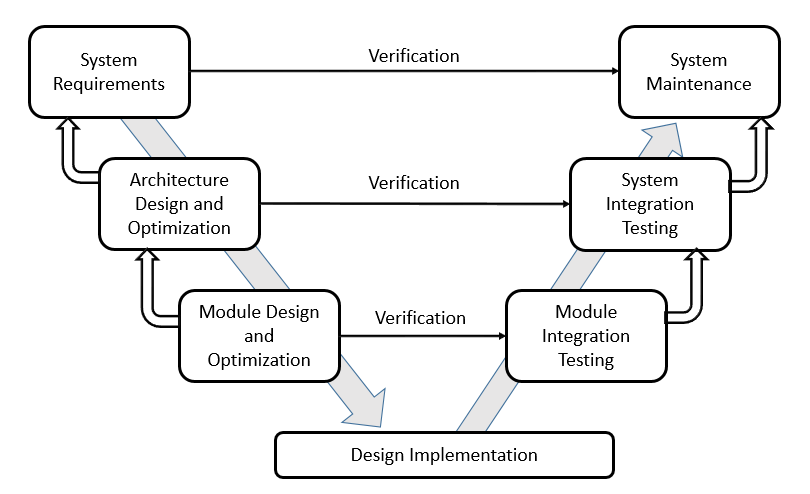
\includegraphics[width=0.85\textwidth] {images/v1.png}}
        \caption{\label{fig:v1} The V Model in System Development}
\end{figure}

\subsection{Traditional Safety Assessment Process}
ARP4754A, the Guidelines for Development of Civil Aircraft and Systems~\cite{SAE:ARP4754A}, provides guidance on applying development assurance at each hierarchical level throughout the development life cycle of highly-integrated/complex aircraft systems. It has been recognized by the Federal Aviation Administration (FAA) as an acceptable method to establish the assurance process. The safety assessment process is a starting point at each hierarchical level of the development life cycle and is tightly coupled with the system development and verification processes. It is used to show compliance with certification requirements and for meeting a company's internal safety standards. 

\begin{figure}[!htb]
        \center{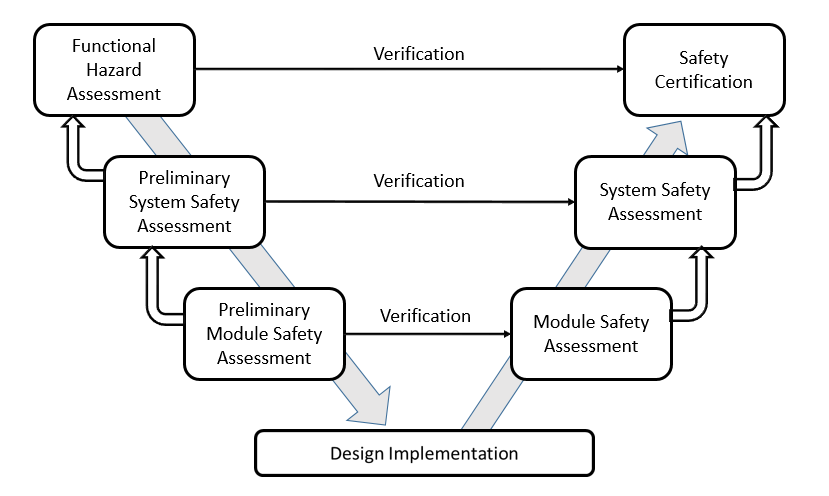
\includegraphics[width=0.85\textwidth] {images/v2.png}}
        \caption{\label{fig:v2} The V Model in Safety Assessment}
\end{figure}

The safety assessment shown in Figure~\ref{fig:v2} integrates each phase of the V model with analyses specific to system hazards and their severity. It also shows how these hazards should be addressed within the design phase. The safety assessment proess is defined in ARP4754A by the following phases:

\begin{description}
\item[Functional Hazard Assessment (FHA)] examines the functions of the system to identify potential functional failures and classifies the potential hazards associated with them. This includes identification of failure conditions, identifying the effects of those failures, classification of each failure condition, and assignment to safety objectives.

\item[Common Cause Analysis (CCA)] verifies and establishes physical and functional separation, isolation, and independence requirements between subsystems and verifies that these requirements have been met.

\item[Preliminary Aircraft Safety Assessment (PASA)] establishes aircraft safety requirements and provide a preliminary indication that the aircraft can meet those safety requirements.

\item[Preliminary System Safety Assessment (PSSA)] examines the proposed architecture(s) to determine how failures could cause the failure conditions determined by the FHA. The objective is to complete the safety requirements of an aircraft or system and show that the proposed system architecture satisfies the safety requirements. The PSSA is an iterative process that is performed at multiple stages of system development. 

\item[Fault Tree Analysis (FTA)] is performed to find combinations of faults that lead to the violation of a safety requirement. The fault tree itself shows the logical relation between the sets of faults and the violation of a safety requirement.

\item[Common Mode Analysis (CMA)] analyzes designs and implementations for elements that may defeat the redundancy
or independence of functions within the design, i.e. if elements are shown as independent in FTA, make sure they are truly independent in the system under consideration.

\item[Failure Modes and Effect Analysis (FMEA)] aims at finding the causality relationship between sets of faults, intermediate events, and undesired states in the system. Usually this is represented in tabular form and called an \textit{FMEA table}.

\item[Aircraft Safety Assessment (ASA)/System Safety Assessment (SSA)] verifies that the system (or aircraft), as implemented, meets the safety requirements specified by the PSSA.

\end{description}
\danielle{AADL/agree}

\subsection{Model Based Safety Assessment}
\label{subsec:mbsa}

The lack of precise models of the system architecture and its failure modes often forces safety analysts to devote significant effort to gathering architectural details about the system behavior from multiple sources. Furthermore, this investigation typically stops at system level, leaving software function details largely unexplored. Typically equipped with the domain knowledge about the system, but not detailed knowledge of how the software applications are designed, practicing safety engineers find it a time consuming and involved process to acquire the knowledge about the behavior of the software applications hosted in a system and its impact on the overall system behavior. A diagram of this process is shown in Figure~\ref{fig:proposed_safety_process}.

\begin{figure}[h]
	\centering
	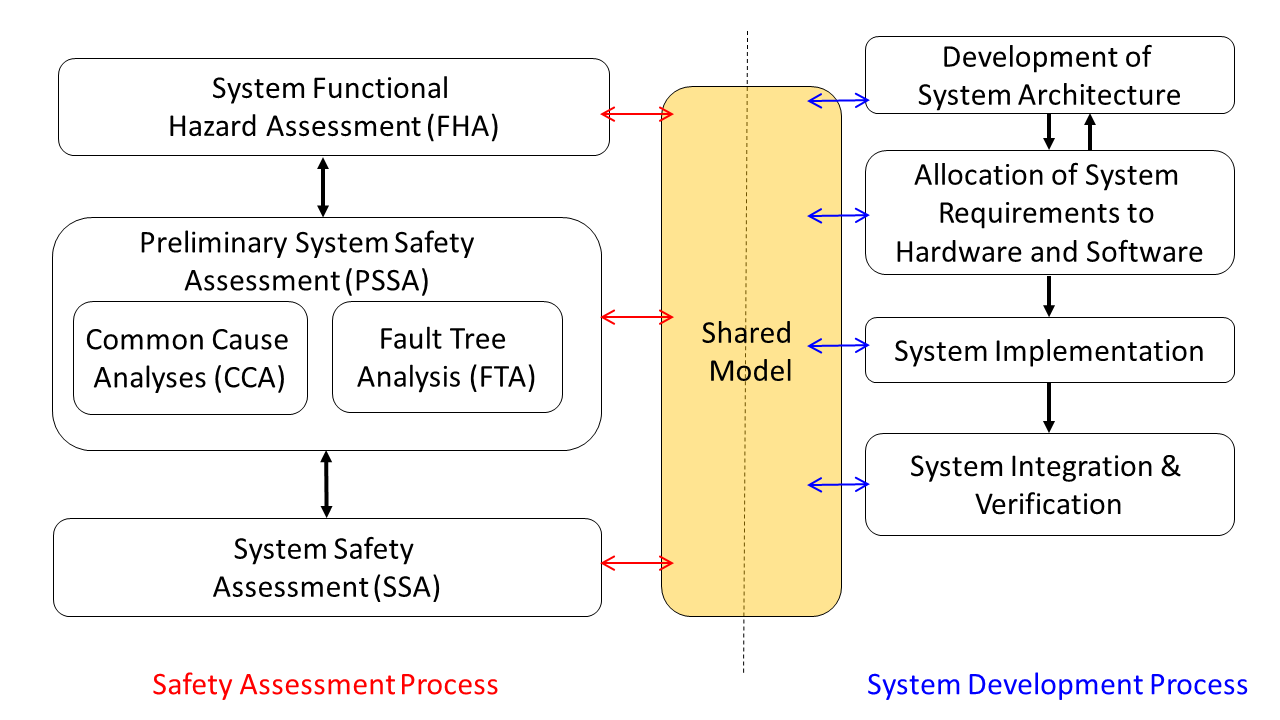
\includegraphics[trim=0 5 0 5,clip,width=0.85\textwidth]{images/process3.png}
	\caption{Use of the Shared System/Safety Model in the ARP4754A Safety Assessment Process}
	\label{fig:proposed_safety_process}
\end{figure}

Industry practitioners have come to realize the benefits of using models in the safety assessment process, and a revision of the ARP4761 to include Model Based Safety Analysis (MBSA) is under way. 

\subsection{Suggested Model Based Safety Assessment Process Supported by Formal Methods}
We propose a model-based safety assessment process backed by formal methods to help safety engineers with early detection of the design issues.  This process uses a single unified model to support both system design and safety analysis; this is shown in Figure~\ref{fig:SACycle1} and is based on the following steps:

\begin{enumerate}
	\item System engineers capture the critical information in a shared model:  high-level hardware and software architecture, nominal behavior at the component level, and safety requirements at the system level.
	\item System engineers use a model checker to check that the safety requirements are satisfied by the nominal design model. 
	\item Safety engineers augment the nominal model with the component failure modes. In addition, safety engineers specify the fault hypothesis for the analysis which corresponds to how many simultaneous faults the system must be able to tolerate.
	\item Safety engineers use a model checker to analyze if the safety requirements and fault tolerance objectives are satisfied by the design in the presence of faults. If the design does not tolerate the specified number of faults (or probability threshold of fault occurrence), then the tool produces counterexamples or minimal sets of fault combinations that can cause the safety requirement to be violated.
	\item The safety engineers examine the results to assess the validity of the fault combinations and the fault tolerance level of the system design. If a design change is warranted, the model will be updated with the latest design change and the above process is repeated.
\end{enumerate}

\begin{figure}[h]
	\begin{center}
		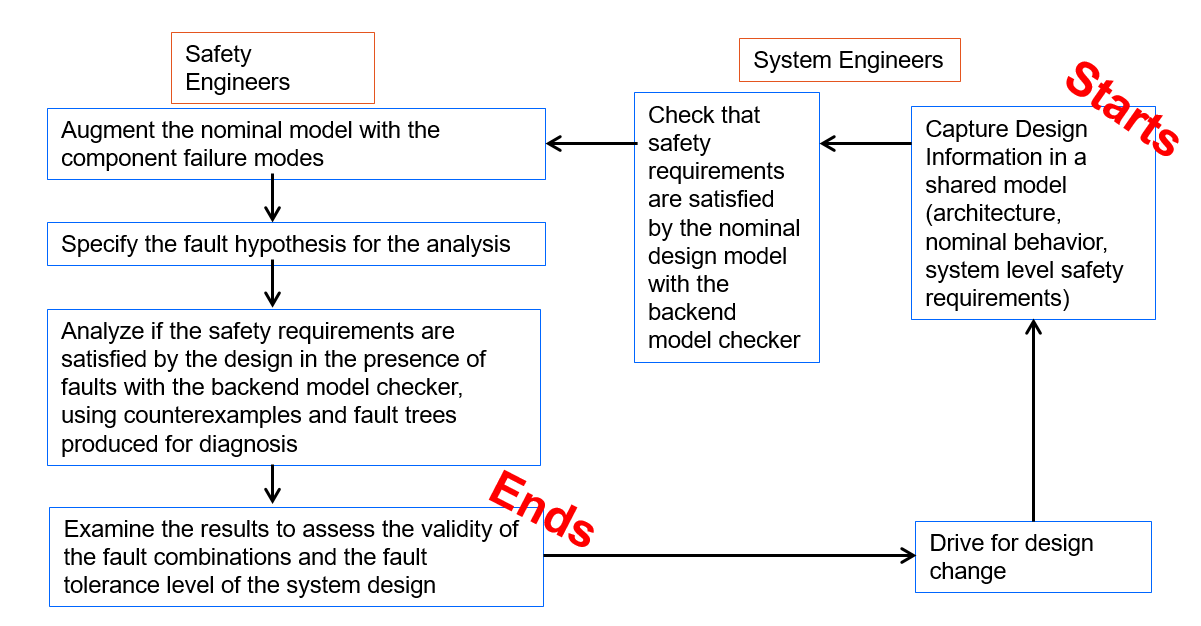
\includegraphics[width=\textwidth]{images/SACycle.PNG}
	\end{center}
	\caption{Proposed Steps of the Safety Assessment Process}
	\label{fig:SACycle1}
\end{figure}

These steps can be viewed as a cyclical process that involves both the system development engineers and the safety engineers of the system. Figure~\ref{fig:SACycle1} shows these steps within the context of the start and end of a project. 

\danielle{Add a bit more information here - pull from the MBSE project for IRAD. Include reasons why this approach is better, how it will help safety analysts, how it benefits the field as a whole. Then lead into the next sections with a statement about model checking, verification, etc.}
subsection{Critical System Development Artifacts}
\label{subsec:crisysArtifacts}












\begin{comment}
ARP4754A, the Guidelines for Development of Civil Aircraft and Systems~\cite{SAE:ARP4754A}, provides guidance on applying development assurance at each hierarchical level throughout the development life cycle of highly-integrated/complex aircraft systems. It has been recognized by the Federal Aviation Administration (FAA) as an acceptable method to establish the assurance process. The safety assessment process is a starting point at each hierarchical level of the development life cycle and is tightly coupled with the system development and verification processes. It is used to show compliance with certification requirements and for meeting a company's internal safety standards. 

ARP4761, the Guidelines and Methods for Conducting Safety Assessment Process on Civil Airborne Systems and Equipment~\cite{SAE:ARP4761},  identifies a systematic means to show compliance. Among the industry accepted safety assessment processes are Preliminary System Safety Assessment (PSSA) and System Safety Assessment (SSA). PSSA evaluates the system design and defines safety requirements. SSA evaluates the implemented system to show that safety requirements defined in the PSSA are in fact satisfied.

A prerequisite of performing the safety assessment is understanding how the system is intended to work, primarily focusing on the integrity of the outputs and the availability of the system. The safety engineers then use the acquired understanding to conduct safety analysis, construct safety analysis artifacts, and compare the results with established safety objectives and requirements.
Typically equipped with the domain knowledge about the system, but not detailed knowledge of how the software applications are designed, practicing safety engineers find it a time consuming and involved process to acquire the knowledge about the behavior of the software applications hosted in a system and its impact on the overall system behavior.
Industry practitioners have come to realize the benefits of using models in the safety assessment process, and a revision of the ARP4761 to include Model Based Safety Analysis (MBSA) is under way.
Figure~\ref{fig:proposed_safety_process} presents our proposed use of a single unified model to support both system design and safety analysis. It describes both system design and safety-relevant information 
that are kept distinguishable and yet are able to interact with each other. The shared model maintains a living model that captures the current state of the system design as it moves through the development lifecycle, allowing all participants of the ARP4754A process to be able to communicate and review the system design. Safety analysis artifacts can be generated directly from the model, 
providing
the capability to more accurately analyze complex systems.

\begin{figure}[t!]
	
	\centering
	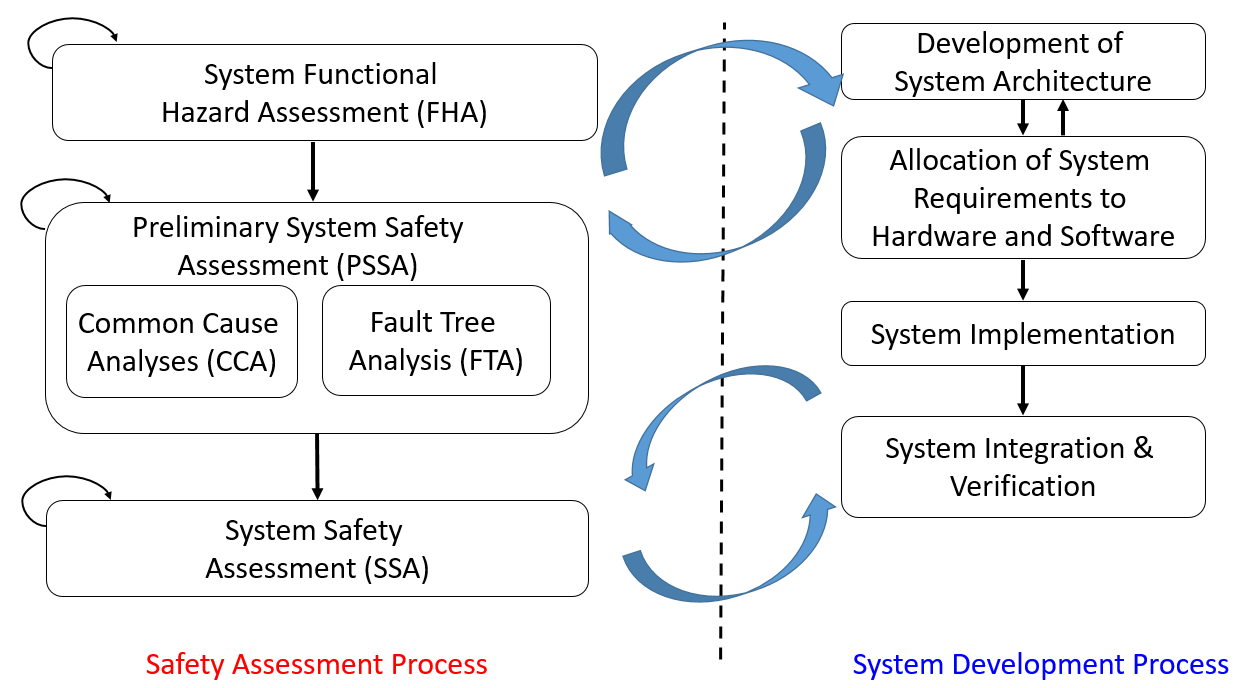
\includegraphics[trim=0 5 0 5,clip,width=0.85\textwidth]{images/process1.png}
	
	\caption{The ARP4754A Safety Assessment Process}
	\label{fig:safety_process}
\end{figure}

\begin{figure}[t!]
	
	\centering
	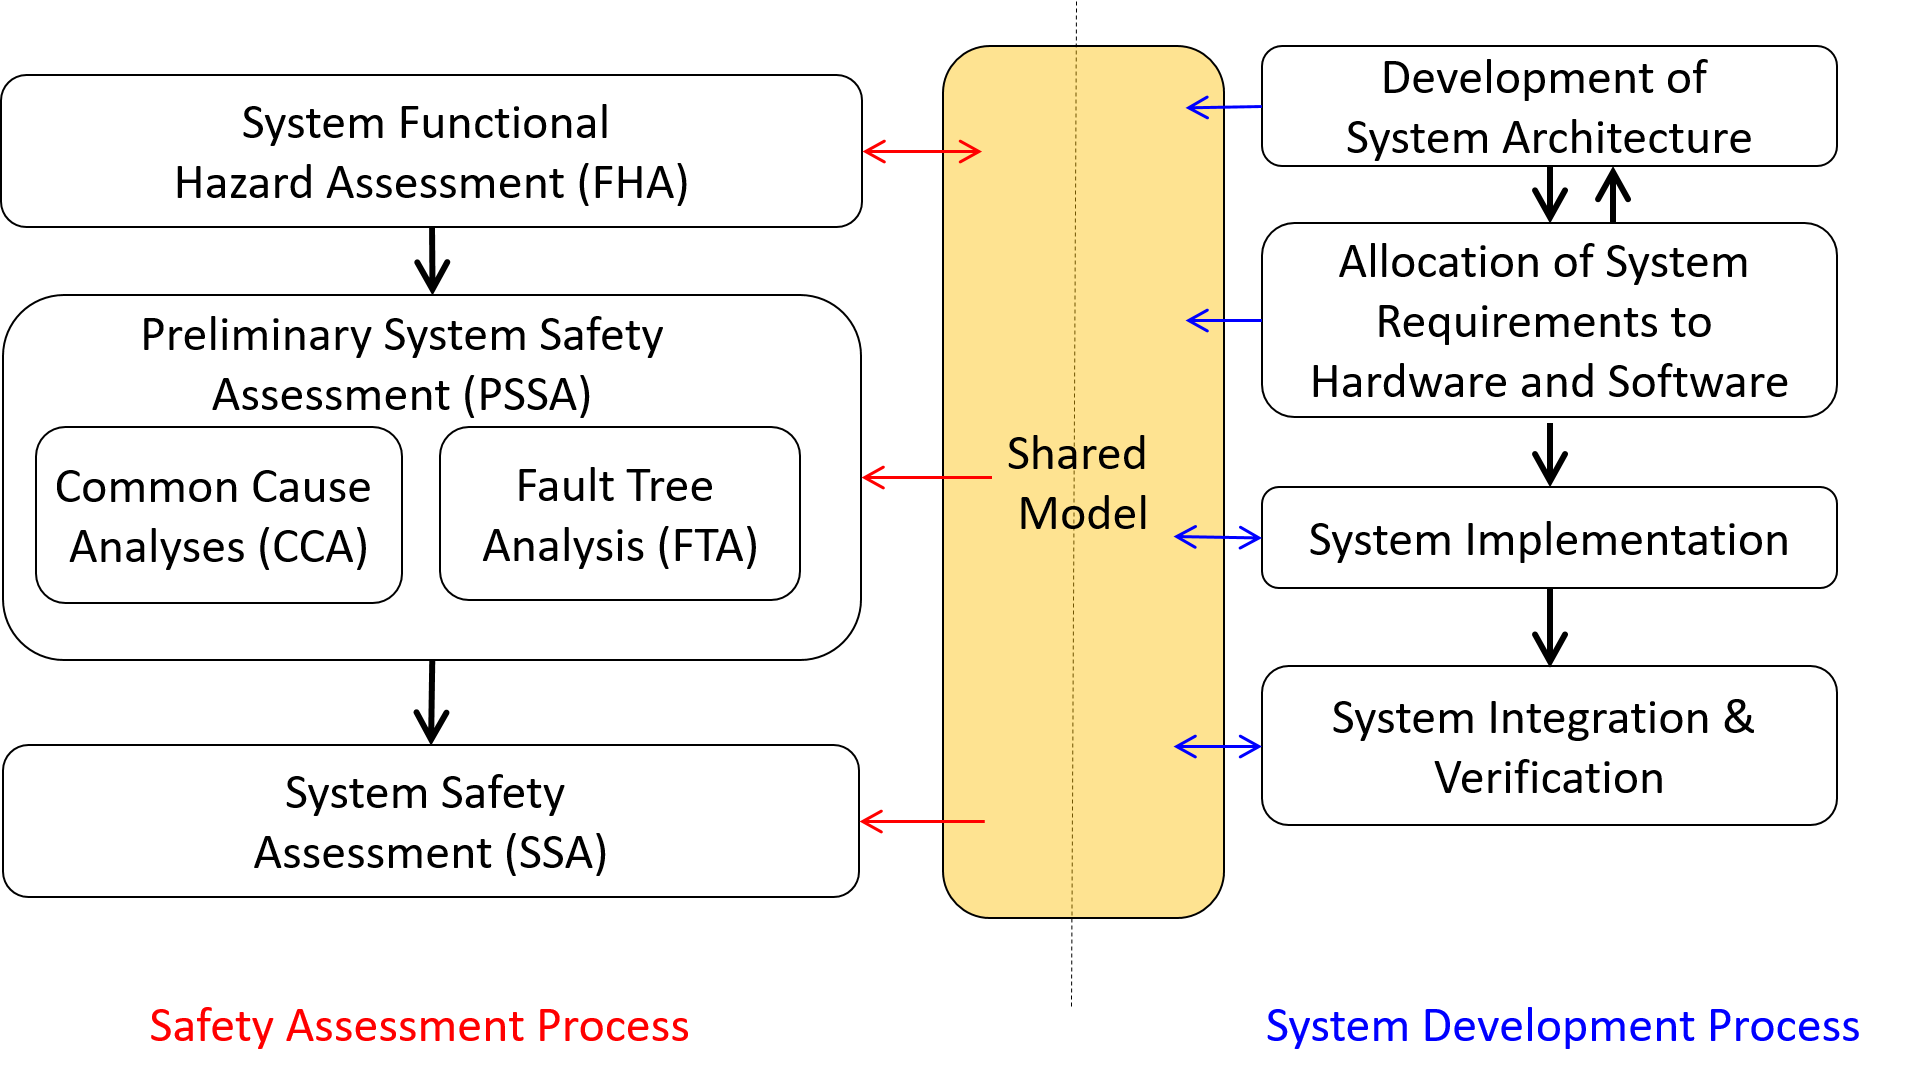
\includegraphics[trim=0 5 0 5,clip,width=0.85\textwidth]{images/process2.png}
	
	\caption{Use of the Shared System/Safety Model in the ARP4754A Safety Assessment Process}
	\label{fig:proposed_safety_process}
\end{figure}
\end{comment}
\subsection{Model Based Safety Assessment}
\label{subsec:mbsa}

The lack of precise models of the system architecture and its failure modes often forces safety analysts to devote significant effort to gathering architectural details about the system behavior from multiple sources. Furthermore, this investigation typically stops at system level, leaving software function details largely unexplored. Typically equipped with the domain knowledge about the system, but not detailed knowledge of how the software applications are designed, practicing safety engineers find it a time consuming and involved process to acquire the knowledge about the behavior of the software applications hosted in a system and its impact on the overall system behavior. A diagram of this process is shown in Figure~\ref{fig:proposed_safety_process}.

\begin{figure}[h]
	\centering
	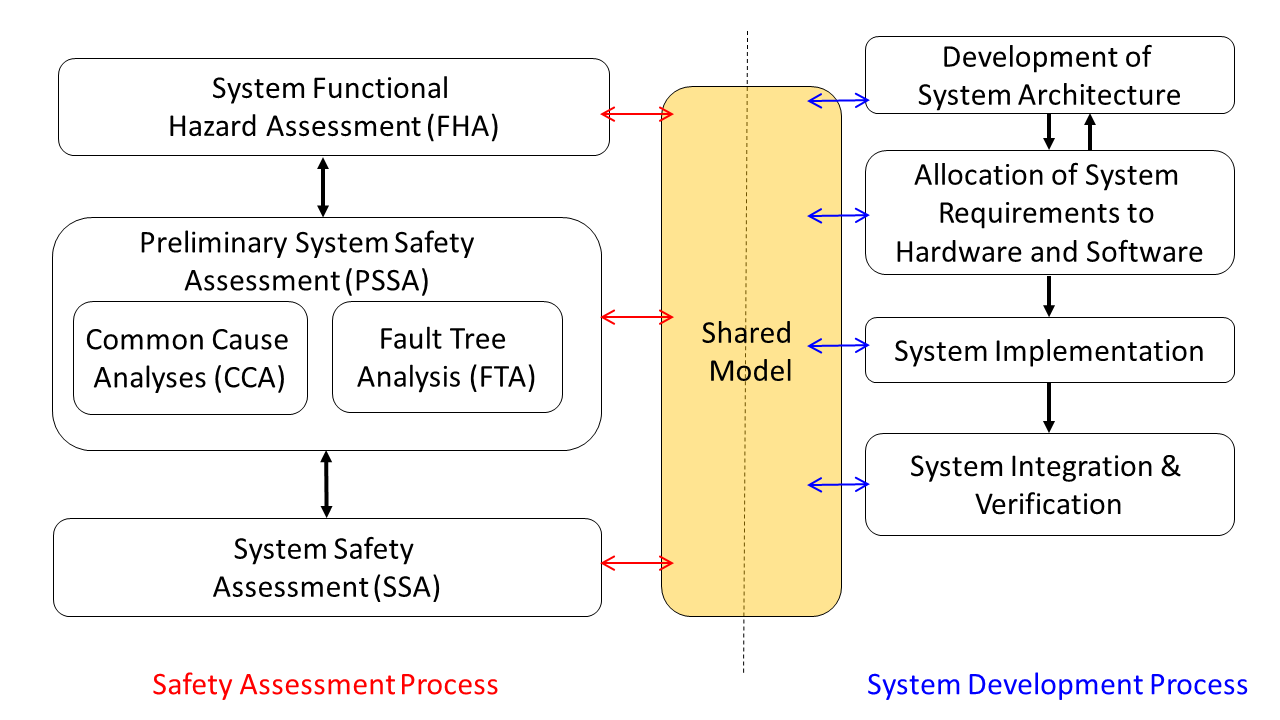
\includegraphics[trim=0 5 0 5,clip,width=0.85\textwidth]{images/process3.png}
	\caption{Use of the Shared System/Safety Model in the ARP4754A Safety Assessment Process}
	\label{fig:proposed_safety_process}
\end{figure}

Industry practitioners have come to realize the benefits of using models in the safety assessment process, and a revision of the ARP4761 to include Model Based Safety Analysis (MBSA) is under way. 

\subsection{Suggested Model Based Safety Assessment Process Supported by Formal Methods}
We propose a model-based safety assessment process backed by formal methods to help safety engineers with early detection of the design issues.  This process uses a single unified model to support both system design and safety analysis; this is shown in Figure~\ref{fig:SACycle1} and is based on the following steps:

\begin{enumerate}
	\item System engineers capture the critical information in a shared model:  high-level hardware and software architecture, nominal behavior at the component level, and safety requirements at the system level.
	\item System engineers use a model checker to check that the safety requirements are satisfied by the nominal design model. 
	\item Safety engineers augment the nominal model with the component failure modes. In addition, safety engineers specify the fault hypothesis for the analysis which corresponds to how many simultaneous faults the system must be able to tolerate.
	\item Safety engineers use a model checker to analyze if the safety requirements and fault tolerance objectives are satisfied by the design in the presence of faults. If the design does not tolerate the specified number of faults (or probability threshold of fault occurrence), then the tool produces counterexamples or minimal sets of fault combinations that can cause the safety requirement to be violated.
	\item The safety engineers examine the results to assess the validity of the fault combinations and the fault tolerance level of the system design. If a design change is warranted, the model will be updated with the latest design change and the above process is repeated.
\end{enumerate}

\begin{figure}[h]
	\begin{center}
		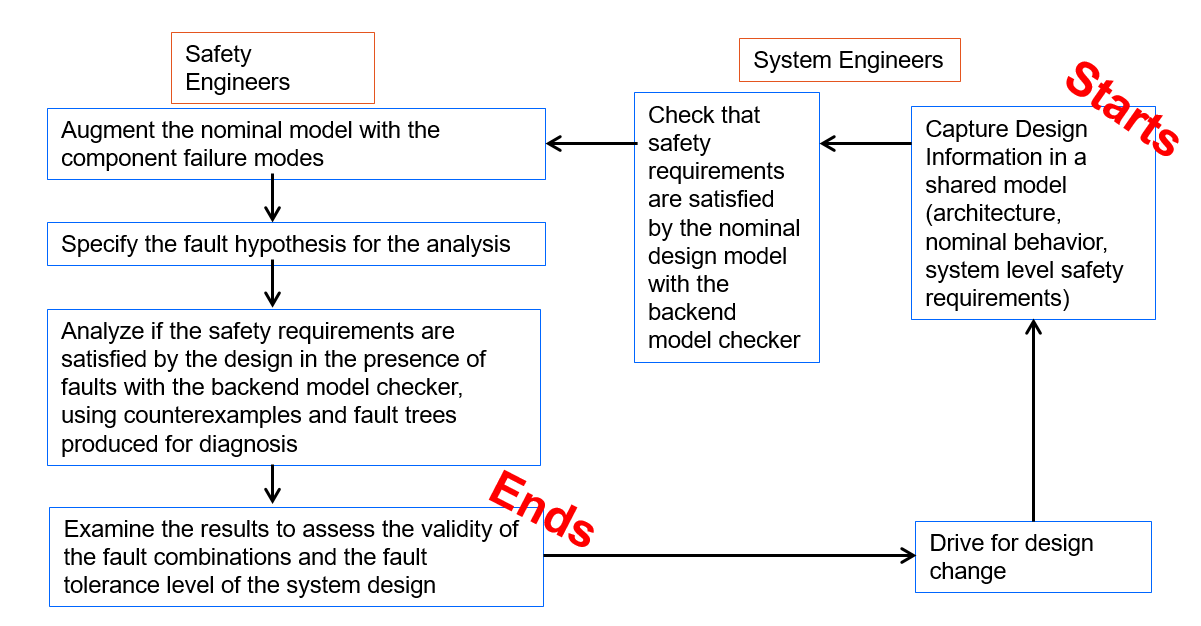
\includegraphics[width=\textwidth]{images/SACycle.PNG}
	\end{center}
	\caption{Proposed Steps of the Safety Assessment Process}
	\label{fig:SACycle1}
\end{figure}

These steps can be viewed as a cyclical process that involves both the system development engineers and the safety engineers of the system. Figure~\ref{fig:SACycle1} shows these steps within the context of the start and end of a project. 

\danielle{Add a bit more information here - pull from the MBSE project for IRAD. Include reasons why this approach is better, how it will help safety analysts, how it benefits the field as a whole. Then lead into the next sections with a statement about model checking, verification, etc.}
\subsection{Overview}
Formal validation and verification is a proof-based methodology used to assess the correctness of requirements, system design, and implementation. In the past, this has been performed through manual means, but with the advancement in automated theorem proving and other formal methods, automated formal analyses not only guarantees a higher degree of confidence, but also reduces the time (and thus cost) of carrying out the proofs of correctness. Techniques used in formal validation and verification include automated theorem proving, model checking, and abstract interpretation. 

\subsubsection{Formal Specification}
Formal specification process translates the informal system requirements into a mathematical logic to determine if the system design is correct~\cite{hinchey2012industrial}. This process guarantees an unambiguous description of the requirements which is not possible when using an informal natural language. This formal definition of system requirements includes the system design and its expected behavior as well as the assumptions on environment. A design or implementation can never be considered correct in isolation; it is only correct with respect to the specifications. The expected behavior, system design, and environmental assumptions change and are refined as the system goes through the various stages of development. 

\subsubsection{Formal Verification} 
Formal verification is the use of proof methods to show that given the environmental assumptions stated in the formal specification, the formal design of the system meets the requirements. The problem can be reduced to that of property checking: given a program $P$ and a specific property, does the program satisfy the given property~\cite{fitting2012first}. This is an undecidable problem because a program can be represented as an infinite state space. The problem is that of finding a finite set of predicates that support the specified property over an infinite state space. This is an undecidable problem; any algorithm searching for a solution to this problem may not terminate~\cite{clarke2018model}. The approaches used to provide these proofs are usually deductive methods or an exhaustive exploration of the model known as model checking. 

Model checking was introduced in the early 1980's and consists of exploring the states and transitions of a model~\cite{clarke1981design,queille1982specification}. By representing the system abstractly, the infinite state space is reduced to a finite model. This addresses the undecidability factor~\cite{d2008survey}. The proofs are generated over an abstract mathematical model of the system, such as finite state machines, labeled transition systems, or timed automata. It takes as input a model of a system and the properties written in propositional temporal logic, then explores the entire state space of the system to determine if the model violates the properties~\cite{clarke2018model,fraser2009testing}. In recent years, model checking takes advantage of abstraction techniques specific to a domain to consider multiple states or transitions in a single operation; this lessens computation time considerably~\cite{d2008survey}. Nevertheless, the biggest limiting factor of model checking is scalability and much of the recent research in this area attempts to address this problem~\cite{clarke2018model}.

Deductive methods of verification consists of generating proof obligations from the specifications of the system and using these obligations in a theorem prover setting. Automated theorem provers have the main objective to show that some statement (conjecture) is a logical consequence of other statements (the axioms and hypotheses). The rules of inference are given as are the set of axioms and hypotheses~\cite{d2008survey,fitting2012first}. Deductive methods of verification include automated theorem provers (e.g., Coq~\cite{coq}, Isabelle~\cite{isabelle}) and satisfiability modulo theories (e.g., SMTInterpol~\cite{smtInterpol}, Z3~\cite{z3}, Yices~\cite{yices}). 


 
\section{Satisfiability}
\label{sec:sat}
The Boolean Satisfiability (SAT) problem attempts to determine if there exists a total truth assignment to a given propositional formula, that evaluates to $true$. Generally, a propositional formula is any combination of the disjunction and conjunction of literals (as an example, $a$ and $\neg a$ are literals). For example, the proposition $a \land b$ is satisfiable; when $a$ and $b$ are assigned to $true$, the formula is satisfied.  On the other hand, the proposition $a \land \neg a$ is unsatisfiable; no such assignment can be found to satisfy both $a$ and $\neg a$. SAT solvers in work over a constraint system of propositional logic to determine satisfiability. Satisfiability Modulo Theories (SMT) solvers also address the SAT problem, but can work over propositional logic or predicate logic with quantifiers. An SMT solver works over a conjunction of literals, as is the case with SAT solvers, but the literals can be expressed as predicates over non-boolean variables, such as $x > 0$. A boolean literal can be satisfied with a finite number of possible assignments; this is not always the case with SMT formula.

\subsection{UNSAT Cores and Minimal Unsatisfiable Subsets}
A constraint system $C$ is an ordered set of $n$ abstract constraints $\{C_1, C_2, ..., C_n\}$ over a set of variables. The constraint $C_i$ restricts the allowed assignments of these variables in some way~\cite{liffiton2016fast}. Given a constraint system, we require some method of determining, for any subset $S \subseteq C$, whether $S$ is \textit{satisfiable} (SAT) or \textit{unsatisfiable} (UNSAT). Given a constraint system $C$, there are certain subsets of $C$ that are of interest in terms of satisfiability. %Definitions 2-4 are taken from research by Liffiton et. al.~\cite{liffiton2016fast}. 

For a given unsatisfiable problem, SAT solvers (and SMT solvers) attempt to provide proof of unsatisfiability by providing a subset of UNSAT clauses known as \textit{UNSAT cores}. In general, this is useful information to have regarding the constraint system in question. 

\begin{definition} A Minimal Unsatisfiable Subset (MUS) $M$ of a finite constraint system $C$ is a subset $M \subseteq C$ such that $M$ is unsatisfiable and $\forall c \in M$ : $M \setminus \{c\}$ is satisfiable. 
\end{definition}

\begin{definition} UNSAT core: Let $C$ be a finite set of constraints and $U \subseteq C$ an unsatisfiable subset. A constraint $c \in U$ is an UNSAT core for $U$ if $U \setminus \{c\}$ is satisfiable. A set of all unsatisfiability cores of $U$ constitute an MUS for $C$. 
\end{definition}

Intuitively, an MUS is the minimal explanation of the constraint systems infeasability and the UNSAT cores are the building blocks of the MUS. In recent years, a number of efficient algorithms have been introduced to find MUSs~\cite{liffiton2005max} and most of them focus on finding a single such subset~\cite{belov2012towards, belov2013core, belov2012muser2}. More recently, algorithms have been introduced that can find all such minimal unsatisfiable subsets~\cite{GhassabaniGW16, Ghassabani2017EfficientGO,bendik2018online}. 

\subsection{Inductive Validity Cores} Given a complex model, it is useful to extract traceability information related to the proof; in other words, which elements of the model were necessary to construct the proof. An algorithm was introduced by Ghassabani et al. to provide Inductive Validity Cores (IVC) as a way to determine which model elements are necessary for the inductive proofs of the safety properties for sequential systems~\cite{GhassabaniGW16}. Given a safety property of the system, a model checker is invoked to construct a proof of the property. The IVC generation algorithm extracts traceability information from the proof process and returns a minimal set of the model elements required in order to prove the property. Later research extended this algorithm in order to produce all minimal IVC elements (\aivcalg)~\cite{Ghassabani2017EfficientGO,bendik2018online}. 

The \aivcalg algorithm considers a constraint system consisting of the assumptions and contracts of system components and the negation of the safety property of interest (i.e. the top level event). It then collects all Minimal Unsatisfiable Subsets (MUSs) of this constraint system; these are the minimal explanations of the constraint systems infeasibility in terms of the \textit{negation} of the safety property. Equivalently, these are the minimal model elements necessary to prove the safety property. 

\subsection{Ordered Binary Decision Diagrams}
A Binary Decision Diagram (BDD) is a data structure used to encode Boolean formulae.
\begin{figure}[!htb]
        \center{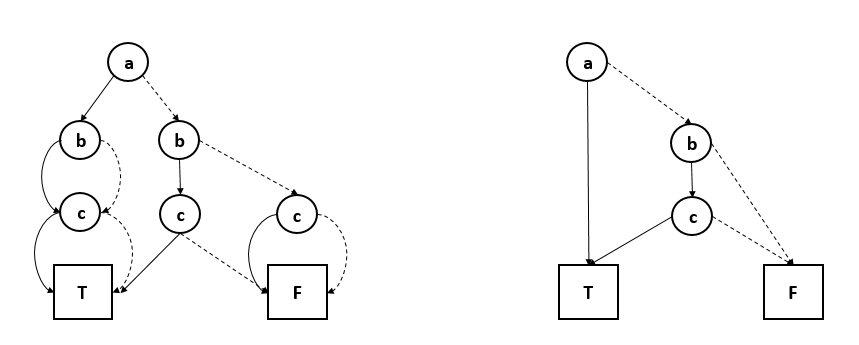
\includegraphics[width=0.8\textwidth] {images/bdd.png}}
        \caption{\label{fig:bdd} Binary Decision Diagrams of the Formula $a \lor (b \land c)$}
\end{figure}
As shown in Figure~\ref{fig:bdd}, it is a rooted, directed, acyclic graph with internal decision nodes and two terminal nodes (\textit{true} and \textit{false}). Each of the decision nodes is labeled with a Boolean variable and has two child nodes, low child and high child. The edge from a node to its low child represents the assignment of \textit{false}, likewise the edge to the high child represents the assignment of \textit{true}. The BDD is called \textit{ordered} if different variables appear in the same order on all paths from the root. Intuitively, following a path from the root to the \textit{true} terminal node represents a valid assignment to the Boolean formula (invalid in the case of ending on the \textit{false} terminal node). 

BDDs can also be reduced by the removal of isomorphic subgraphs. The BDD shown on the right of Figure~\ref{fig:bdd} is the reduced form of the BDD on the left. 












\section{Formal Methods in Safety Analysis: A Brief History and the State of the Practice}
\label{sec:modelCheckingInSA}
Safety analysis has traditionally been performed manually, but with the rise of model checking and the improvement of its capabilities, the world of safety analysis began to see its powerful benefits~\cite{hinchey2012industrial, liggesmeyer1998improving, coudert1993fault, Bozzano:2010:DSA:1951720,bozzano2003esacs}. There arose multiple ways of viewing the system and fault models, various ways of automating the capture of safety pertinent information, and a number of tools that addressed various issues that arose. In this section, we discuss the state of the practice and how formal methods has been applied in the domain of safety assessment research.

\subsection{Model Checking in Model Based Safety Analysis}
From the beginnings of model checking, there was a slow increase in its application to the domain of safety analysis, but a few research groups contributed immensely to this branch of study. Separately, these researchers began to contribute to safety analysis through the use of model checking starting in the '90's and are still contributing today (e.g., \cite{reese1997software,signoret1998altarica,chiappini1999formal,cimatti2000industrial}. 

One of the main methods was the abstraction of the system into a formal transition system; this provided a means of defining a precise mathematical model of the system and simplifying mathematical operations through the use of abstraction techniques on the transition system. This helped to shrink the entire state space into something more digestible by computational techniques~\cite{d2008survey}. 

In the early 2000's, model based safety assessment began to make an appearance in literature~\cite{Bozzano:2010:DSA:1951720,Joshi05:Dasc, Joshi05:SafeComp, Joshi07:Hase}. This applied model checking and model based system development to safety analysis at the same time.  In this approach, a safety analysis system model (SASM) is the central artifact in the safety analysis process, and traditional safety analysis artifacts, such as fault trees, are automatically generated by tools that analyze the SASM.

The contents and structure of the SASM differ significantly across different conceptions of MBSA.  We can draw distinctions between approaches along several different axes.  The first is whether they propagate faults explicitly through user-defined propagations, which we call {\em failure logic modeling} (FLM), or {\em explicit propagation}, or through existing behavioral modeling, which we call {\em failure effect modeling} (FEM), or {\em implicit propagation}.  The next is whether models and notations are {\em purpose-built} for safety analysis vs. those that extend {\em existing system models} (ESM).

For FEM approaches, there are several additional dimensions.  One dimension involves whether {\em causal} or {\em non-causal} models are allowed.  Non-causal models allow simultaneous (in time) bi-directional error propagations, which allow more natural expression of some failure types (e.g. reverse flow within segments of a pipe), but are more difficult to analyze.  A final dimension involves whether analysis is {\em compositional} across layers of hierarchically-composed systems or {\em monolithic}.  %Our approach is an extension of AADL (ESM), causal, compositional, mixed FLM/FEM approach.
\danielle{Make a figure here - that will help explain these distinctions.}

This literature overview is not a complete account of all safety analysis model checking tools available either in industry or research, but highlights some of the most influential safety assessment methods and tools currently available. 

\subsubsection{AltaRica}
AltaRica was one of the first model checking tools specifically aimed at safety analysis of critical systems. The first iteration of AltaRica (1.0) performed over a transition system of the model, used dataflow ({\em causal}) semantics, and could capture the hierarchy of a system~\cite{signoret1998altarica}. The key idea was that this transition system (more specifically {\em constraint automata}) could be compiled into Boolean formulae and transformed into a BDD~\cite{point1999altarica}. The literature for performing fault tree analysis over BDDs was rich with algorithms; this was how much of the safety analysis artifacts were generated. The dataflow dialect (AltaRica 1.0) has substantial tool support, including the commercial Cecilia OCAS tool from Dassault~\cite{bieber2004safety}. For this dialect, the safety assessment, fault tree generation, and functional verification can be performed with the aid of NuSMV model checking~\cite{symbAltaRica}.

The most recent language update (AltaRica 3.0) uses non-causal semantics~\cite{prosvirnova2013compilationfaulttrees,PROSVIRNOVA2013127}. Failure states are defined throughout the system and flow variables are updated through the use of assertions~\cite{Bieber04safetyassessment}.  AltaRica 3.0 has support for simulation and Markov model generation through the OpenAltaRica (www.openaltarica.fr) tool suite; it is a {\em FEM}-based, {\em purpose-built}, {\em monolithic} safety analysis language. 

AltaRica 3.0 provides automated fault tree generation by translating the model into a reachability graph and then further compiling it into Boolean formula in order to compute minimal cut sets~\cite{prosvirnova2015automated}. 

\subsubsection{FSAP, xSAP, and COMPASS}
The Formal Safety Analysis Platform (FSAP) was introduced in 2003~\cite{bozzano2003improving} and supported failure mode definitions, safety requirements in temporal logic formulae, automated fault tree construction, and counterexample traces. The platform used NuSMV, a BDD-based model checker~\cite{Cimatti2000}. The system model, written in NuSMV, and the fault model, developed graphically in FSAP, are together translated into a finite state machine and eventually into a BDD; fault tree analysis is performed using BDD algorithms implemented in NuSMV. 

By 2016, the researchers that developed FSAP (Foundation Bruno Kessler, FBK) released a similar tool called xSAP~\cite{DBLP:conf/tacas/BittnerBCCGGMMZ16}. xSAP extends FSAP in many ways: xSAP can handle infinite state machines, it is textual language rather than graphical, allows for richer fault modeling and definitions, and implements more than just BDD computations (e.g., SAT- and SMT-based routines). xSAP was integrated into the COMPASS toolsuite to take advantage of the algorithms it supports. More complex SAT-based algorithms were introduced to bypass the BDD method of minimal cut set generation, namely the ``anytime approximation" algorithms~\cite{CAV2015:BoCiGrMa, mattarei2016scalable}. These algorithms make clever use of bounded model checking algorithms to explore counterexamples provided to the query "the top level event never occurs." These explorations are done such that the cut sets generated are of increasing cardinality which allows for an approximation computation to be given even when the state space is too large to compute all minimal cut sets. These are implemented in xSAP~\cite{CAV2015:BoCiGrMa}.

COMPASS (Correctness, Modeling project and Performance of Aerospace Systems)~\cite{10.1007/978-3-642-04468-7_15} is a mixed {\em FLM/FEM}-based, {\em causal} {\em compositional} tool suite that uses the SLIM language, which is based on a subset of the Architecture Analysis and Design Language (AADL), for its input models~\cite{5185388, criticalembeddedsystems}. In SLIM, a nominal system model and the error model are developed separately and then transformed into an extended system model.  This extended model is automatically translated into input models for the NuSMV model checker~\cite{Cimatti2000, NuSMV}, MRMC (Markov Reward Model Checker)~\cite{Katoen:2005:MRM:1114692.1115230, MRMC}, and RAT (Requirements Analysis Tool)~\cite{RAT}. The safety analysis tool xSAP~\cite{DBLP:conf/tacas/BittnerBCCGGMMZ16} can be invoked in order to generate safety analysis artifacts such as fault trees and FMEA tables~\cite{compass30toolset}.  %COMPASS is an impressive tool suite, but some of the features that make AADL suitable for SW/HW architecture specification: event and event-data ports, threads, and processes, appear to be missing, which means that the SLIM language may not be suitable as a general system design notation (ESM).

\subsubsection{SmartIFlow}
SmartIFlow~\cite{info17:HaLuHo,honig2014new} is a {\em FEM}-based, {\em purpose-built}, {\em monolithic} {\em non-causal} safety analysis tool that describes components and their interactions using finite state machines and events. Verification is done through an explicit state model checker which returns sets of counterexamples for safety requirements in the presence of failures.  SmartIFlow allows {\em non-causal} models containing simultaneous (in time) bi-directional error propagations.  On the other hand, the tools do not yet appear to scale to industrial-sized problems, as mentioned by the authors: ``As current experience is based on models with limited size, there is still a long way to go to make this approach ready for application in an industrial context''~\cite{info17:HaLuHo}.

\subsubsection{SAML}
The Safety Analysis and Modeling Language (SAML)~\cite{Gudemann:2010:FQQ:1909626.1909813} is a {\em FEM}-based, {\em purpose-built}, {\em monolithic} {\em causal} safety analysis language that was developed in 2010.  System models constructed in SAML can be used used for both qualitative and quantitative analyses. It allows for the combination of discrete probability distributions and non-determinism. The SAML model can be automatically imported into several analysis tools like NuSMV~\cite{Cimatti2000}, PRISM (Probabilistic Symbolic Model Checker)~\cite{CAV2011:KwNoPa}, or the MRMC probabilistic model checker~\cite{Katoen:2005:MRM:1114692.1115230}. SAML itself does not provide the formal verification engines, but instead provides a platform to model the safety aspects of a system and then translate this into the input language for a formal verification engine~\cite{Gudemann:2010:FQQ:1909626.1909813}.

\subsubsection{Error Model Annex for AADL}
The SAE (Society of Automotive Engineers) released the
aerospace standard AS5506, named Architecture Analysis and Design Language (AADL), which is a mature industry-standard for embedded systems and has proved to be efficient for architecture modeling~\cite{aerospace2012sae,liu2016research}. AADL supports safety analysis by adding EMA (Error Model Annex) as an extension to the language. EMA allows the user to annotate system hardware and software architectures with hazard, error propagation, failure modes and effects due to failures. Around 2016, Version 2 of the Error Model Annex was released (EMV2)~\cite{EMV2}. EMV2 is an {\em FLM}-based {\em ESM} approach. The faults and error propagations are explicitly defined and the fault tree analysis is performed by traversing propagation paths in reverse to find the original fault that caused the problem~\cite{feiler2017automated}. 



 
	%\section{The Safety Assessment Process}
\label{sec:process}
ARP4754A, the Guidelines for Development of Civil Aircraft and Systems~\cite{SAE:ARP4754A}, provides guidance on applying development assurance at each hierarchical level throughout the development life cycle of highly-integrated/complex aircraft systems. It has been recognized by the Federal Aviation Administration (FAA) as an acceptable method to establish the assurance process. The safety assessment process is a starting point at each hierarchical level of the development life cycle and is tightly coupled with the system development and verification processes. It is used to show compliance with certification requirements and for meeting a company's internal safety standards. 

\begin{figure}[!htb]
        \center{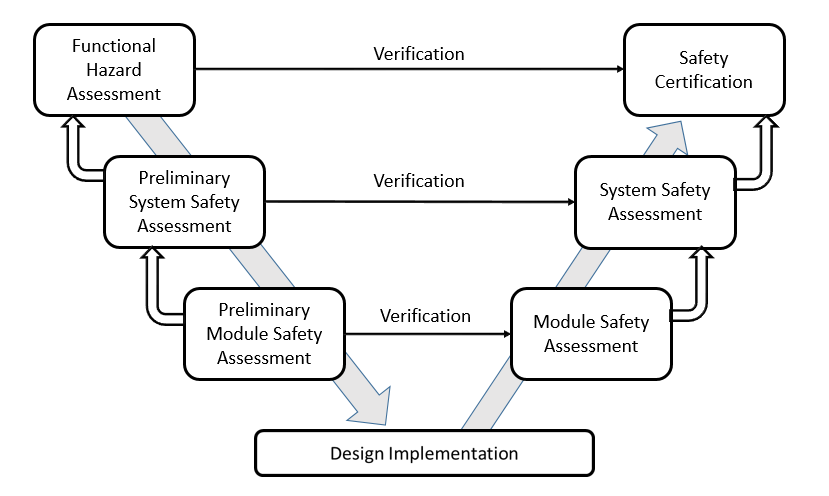
\includegraphics[width=0.85\textwidth] {images/v2.png}}
        \caption{\label{fig:v2} The V Model in Safety Assessment}
\end{figure}

The safety assessment shown in Figure~\ref{fig:v2} integrates each phase of the V model with analyses specific to system hazards and their severity. It also shows how these hazards should be addressed within the design phase. The safety assessment proess is defined in ARP4754A by the following phases:

\begin{description}
\item[Functional Hazard Assessment (FHA)] examines the functions of the system to identify potential functional failures and classifies the potential hazards associated with them. This includes identification of failure conditions, identifying the effects of those failures, classification of each failure condition, and assignment to safety objectives.

\item[Common Cause Analysis (CCA)] verifies and establishes physical and functional separation, isolation, and independence requirements between subsystems and verifies that these requirements have been met.

\item[Preliminary Aircraft Safety Assessment (PASA)] establishes aircraft safety requirements and provide a preliminary indication that the aircraft can meet those safety requirements.

\item[Preliminary System Safety Assessment (PSSA)] examines the proposed architecture(s) to determine how failures could cause the failure conditions determined by the FHA. The objective is to complete the safety requirements of an aircraft or system and show that the proposed system architecture satisfies the safety requirements. The PSSA is an iterative process that is performed at multiple stages of system development. 

\item[Fault Tree Analysis (FTA)] is performed to find combinations of faults that lead to the violation of a safety requirement. The fault tree itself shows the logical relation between the sets of faults and the violation of a safety requirement.

\item[Common Mode Analysis (CMA)] analyzes designs and implementations for elements that may defeat the redundancy
or independence of functions within the design, i.e. if elements are shown as independent in FTA, make sure they are truly independent in the system under consideration.

\item[Failure Modes and Effect Analysis (FMEA)] aims at finding the causality relationship between sets of faults, intermediate events, and undesired states in the system. Usually this is represented in tabular form and called an \textit{FMEA table}.

\item[Aircraft Safety Assessment (ASA)/System Safety Assessment (SSA)] verifies that the system (or aircraft), as implemented, meets the safety requirements specified by the PSSA.

\end{description}

\begin{comment}
\subsection{Proposed Model Based Safety Assessment Process Supported by Formal Methods}
We propose a model-based safety assessment process backed by formal methods to help safety engineers with early detection of the design issues.  This process uses a single unified model to support both system design and safety analysis; this is shown in Figure~\ref{fig:SACycle1} and is based on the following steps:

\begin{enumerate}
	\item System engineers capture the critical information in a shared model:  high-level hardware and software architecture, nominal behavior at the component level, and safety requirements at the system level.
	\item System engineers use a model checker to check that the safety requirements are satisfied by the nominal design model. 
	\item Safety engineers augment the nominal model with the component failure modes. In addition, safety engineers specify the fault hypothesis for the analysis which corresponds to how many simultaneous faults the system must be able to tolerate.
	\item Safety engineers use a model checker to analyze if the safety requirements and fault tolerance objectives are satisfied by the design in the presence of faults. If the design does not tolerate the specified number of faults (or probability threshold of fault occurrence), then the tool produces counterexamples or minimal sets of fault combinations that can cause the safety requirement to be violated.
	\item The safety engineers examine the results to assess the validity of the fault combinations and the fault tolerance level of the system design. If a design change is warranted, the model will be updated with the latest design change and the above process is repeated.
\end{enumerate}

\begin{figure}[h]
	\begin{center}
		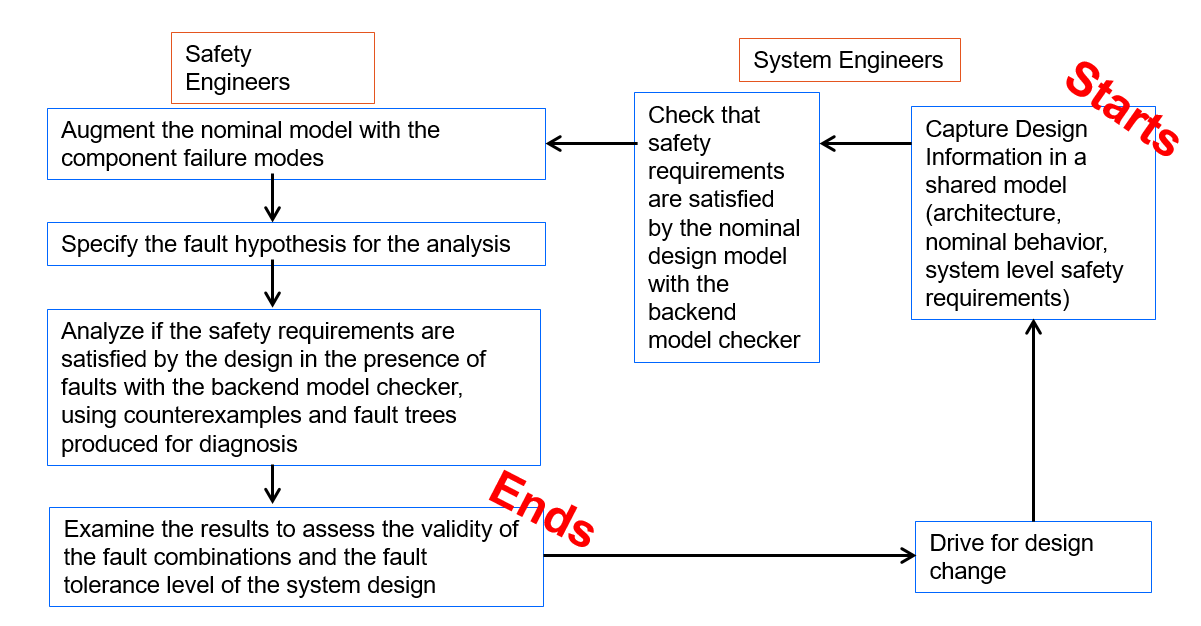
\includegraphics[width=\textwidth]{images/SACycle.PNG}
	\end{center}
	\caption{Proposed Steps of the Safety Assessment Process}
	\label{fig:SACycle1}
\end{figure}

These steps can be viewed as a cyclical process that involves both the system development engineers and the safety engineers of the system. Figure~\ref{fig:SACycle1} shows these steps within the context of the start and end of a project. 

\danielle{Add a bit more information here - pull from the MBSE project for IRAD. Include reasons why this approach is better, how it will help safety analysts, how it benefits the field as a whole. Then lead into the next sections with a statement about model checking, verification, etc.}
\end{comment}
		%\subsection{Fault Forests, Trees, and Minimal Cut Sets}
\label{sec:saArtifacts}
%\danielle{Move this paragraph to where it makes sense.} Safety analysis has traditionally been performed manually, but with the rise of model checking and the improvement of its capabilities, the world of safety analysis began to see its powerful benefits~\cite{hinchey2012industrial, liggesmeyer1998improving, coudert1993fault, Bozzano:2010:DSA:1951720,bozzano2003esacs}. There arose multiple ways of viewing the system and fault models, various ways of automating the capture of safety pertinent information, and a number of tools that addressed various issues that arose. In this section, we discuss the state of the practice and how formal methods has been applied in the domain of safety assessment research.

A \emph{fault tree} is a directed acyclic graph whose leaves model component failures and whose gates model failure propagation. The system failure under examination is the root of the tree and is called the \emph{top level event}. The \emph{basic events} are the events that can occur in the system which lead to the top level event and in the graphical model, these correspond to the leaves. A {\em fault forest} is simply a set of fault trees. The gates in the fault tree describe how failures propagate through the system. Each gate has one output and one or more inputs. In Figure~\ref{fig:introFT}, the AND gate has three inputs and one output. The leaves of the tree represent the basic events of the system and in the case of this fault tree, these three events are also a \textit{minimum cut set} for this top level event. The minimal cut set is the minimal set of basic events that must occur together in order to cause the top level event to occur. Finding these sets is important to fault tree analysis and has been an active area of interest in the research community since fault trees were first described in Bell Labs in 1961~\cite{historyFTA, 0f356f05e72f43018211b36f97c8854a}. 

\begin{figure}[h]
\begin{center}
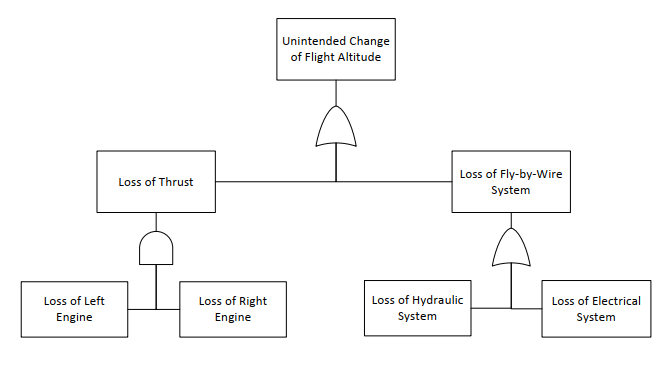
\includegraphics[width=8cm]{images/ft.png}
\caption{A Simple Fault Tree} \label{fig:introFT}
\end{center}
\end{figure}

Figure~\ref{fig:introFT} shows a simple example of a fault tree. In this example, the top level event corresponds to an aircraft having an unintended change of altitude. In order for this event to occur, there must be either a loss of thrust or the loss of a Fly-by-Wire system. This is seen through the use of the OR gate below the top level event. The malfunction of both the left and right engines will cause the loss of thrust to occur and the Fly-by-Wire system can be lost if either the hydraulic system or the electrical system were to malfunction. The MCSs for this example are \{Loss of Left Engine, Loss of Right Engine\}, \{Loss of Hydraulic System\}, and \{Loss of Electrical System\}. 

%There are two main types of FTA that we differentiate here as \textit{qualitative} analysis and \textit{quantitative} analysis. In qualitative analysis, the structure of the fault tree is considered and the cut sets are a way to indicate which combinations of component failures will cause the system to fail. On the other hand, in quantitative analysis the probability of the TLE is calculated given the probability of occurance of the basic events. 

\textbf{History of Fault Trees} 
Since the early days of safety engineering, fault tree analysis has been a primary method of determining safety of a system and showing the behavior of the system (with respect to its requirements) in the presence of faults~\cite{0f356f05e72f43018211b36f97c8854a,vesely1981fault}. Fault tree analysis requires one to explore the faults of the system and their effects on system behavior to determine minimal fault configurations that may violate requirements. From the beginning of fault tree analysis in the 1960s, algorithms worked directly with the fault tree structure to produce minimal cut sets~\cite{10020219108,semanderes1971elraft}. In essence, these algorithms represented each AND/OR gate as a boolean expression and then performed simplification to relate the basic events to the top level event without any gates~\cite{0f356f05e72f43018211b36f97c8854a}. In 1993, Rauzy et al. developed a new approach that converted the fault tree structure into a binary decision diagram (BDD)~\cite{rauzy1993new}. This was a natural way to reduce the Boolean formula into something far more computationally efficient and reducible to even simpler forms. BDDs are still commonly used to perform quantitative and qualitative fault tree analysis~\cite{sinnamon1997new,bryant1986graph,aralia1996computation,reay2002fault,rauzy2007assessment,ge2015quantitative,jiang2018algebraic,banov2019new}.  Other forms of fault tree analysis include Monte Carlo methods~\cite{vesely1970prep}, Markov chains~\cite{boudali2007dynamic}, and zero suppressed BDDs~\cite{minato2001zero}. 




\begin{comment}
\subsubsection{Failure Mode and Effects Analysis}
\danielle{Is this section necessary? If I don't talk about FMEA tables again, cut this.} Failure Mode and Effects Analysis (FMEA) was one of the first systematic ways of performing dependability analysis and is used throughout the safety critical industries~\cite{rausand2003system,Bozzano:2011:SDP:1992983.1992988}. FMEA provides a structured way to list possible failures and their consequences systemwide. If probabilities of failures are known, quantitative analysis can be performed to estimate system reliability and to assign critical significance to potential failure modes or system components~\cite{MilStandardFMEA}. Performing FMEA is often the first step in the fault tree construction, for it shows possible component failures and hence basic events~\cite{0f356f05e72f43018211b36f97c8854a}. Typically, the failure modes of the components at a given level are considered; the objective it to identify the effects of the failure modes at that level - and usually higher levels - of the design. The FMEA results are often presented in tabular form (FMEA Table). FMEA tables vary in form, but almost always include failure mode definitions, the operational mode in which the failure can occur, and possible causes of the failure~\cite{Bozzano:2010:DSA:1951720}.
\end{comment}

		%\subsection{Model Based Development}
\label{sec:mbd}
System safety analysis techniqes are well established and used extensively in the design of safety critical systems. These safety analysis techniques are often performed manually based on informal design models and various other documents~\cite{schatz2002model,Joshi05:Dasc}. Fault trees are one of the most common artifacts used by safety engineers, but different engineers may produce substantially different fault trees for the same system. It becomes clear that the analyses are highly subjective and dependent on the skill of the practitioner. Since the analyses are based on informal system documentation, researchers and practitioners have proposed a consolidation of the information into a central entity and use this to perform safety analysis~\cite{joshi2008behavioral, Joshi05:SafeComp, Joshi07:Hase, CAV2015:BoCiGrMa, Bozzano:2010:DSA:1951720, lisagor2011model}.

One way to achieve consolidation of information spread across various informal documents is through \emph{Model-based Development} (MBD)~\cite{schatz2002model}. In MBD, the development is centered around a formal specification or model of the system. This model can be analyzed for completeness and consistency~\cite{heimdahl1996completeness}, model checking~\cite{miller2010software,clarke2018model, grumberg1994model}, theorem proving~\cite{rayadurgam2003using}, test case generation~\cite{anand2013orchestrated,rayadurgam2001coverage}, etc. One can also automate aspects of the implementation from the formal specification. There are several modeling and verification notations that provide these capabilities. 

Model-based Development can also refer to a process that considers a non-formal model, such as SysML~\cite{friedenthal2014practical} or UML~\cite{fowler2003brief}, as the central development artifact. In this dissertation, we consider a formal model of the system in a language with well-defined semantics as the central artifact of the MBD process. 

While there are numerous modeling languages and specifications both in industry and research, we focus on one for this research: the Architecture Analysis and Design Language. 

\subsubsection{Architecture Analysis and Design Language}
The Architectural Analysis and Design Language (AADL) is an SAE International standard language that provides a unifying framework for describing the system architecture for performance-critical, embedded, real-time systems~\cite{AADL_Standard,FeilerModelBasedEngineering2012}. From its conception, AADL has been designed for the design and construction of avionics systems.  Rather than being merely descriptive, AADL models can be made specific enough to support system-level code generation.  
 
An AADL model describes a system in terms of a hierarchy of components and their interconnections, where each component can either represent a logical entity (e.g., application software functions, data) or a physical entity (e.g., buses, processors). An AADL model can be extended with language annexes to provide a richer set of modeling elements for various system design and analysis needs (e.g., performance-related characteristics, configuration settings, dynamic behaviors). The language definition is sufficiently rigorous to support formal analysis tools that allow for early phase error/fault detection. 

Further details regarding AADL will be introduced as needed throughout this dissertation. 
		%\subsection{Model Based Safety Assessment}
\label{subsec:mbsa}

The lack of precise models of the system architecture and its failure modes often forces safety analysts to devote significant effort to gathering architectural details about the system behavior from multiple sources. Furthermore, this investigation typically stops at system level, leaving software function details largely unexplored. Typically equipped with the domain knowledge about the system, but not detailed knowledge of how the software applications are designed, practicing safety engineers find it a time consuming and involved process to acquire the knowledge about the behavior of the software applications hosted in a system and its impact on the overall system behavior. A diagram of this process is shown in Figure~\ref{fig:proposed_safety_process}.

\begin{figure}[h]
	\centering
	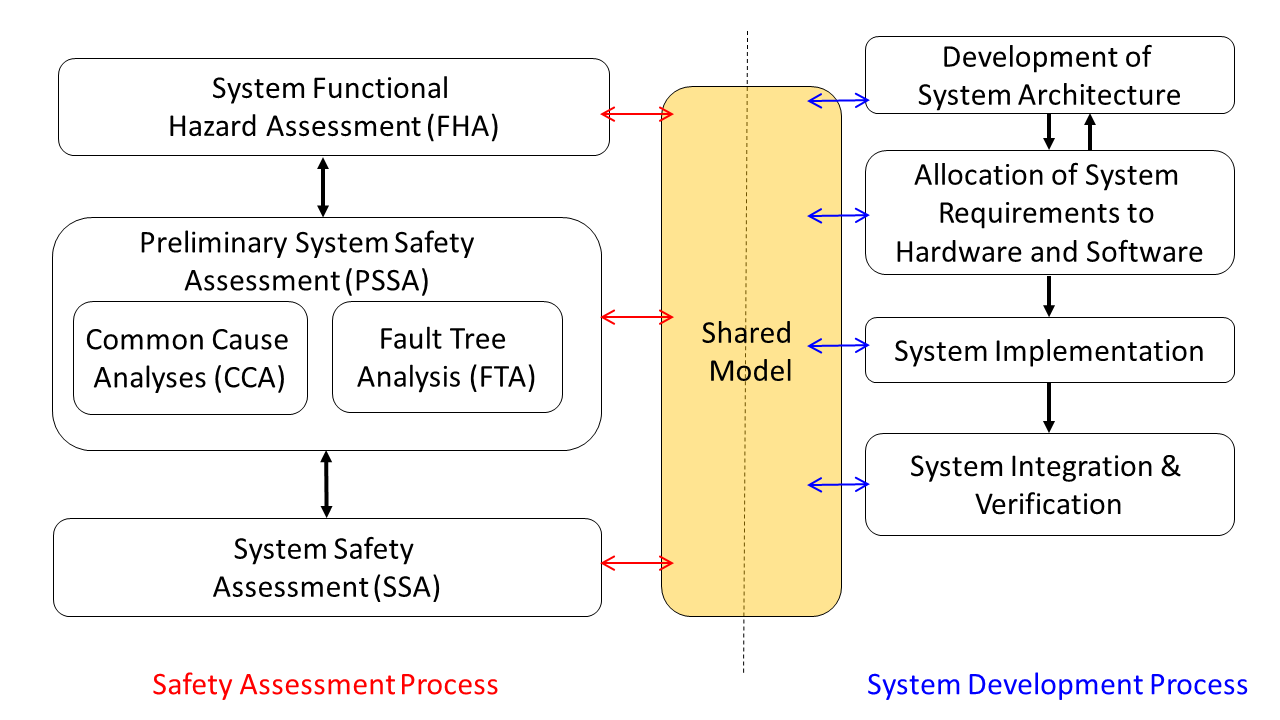
\includegraphics[trim=0 5 0 5,clip,width=0.85\textwidth]{images/process3.png}
	\caption{Use of the Shared System/Safety Model in the ARP4754A Safety Assessment Process}
	\label{fig:proposed_safety_process}
\end{figure}

Industry practitioners have come to realize the benefits of using models in the safety assessment process, and a revision of the ARP4761 to include Model Based Safety Analysis (MBSA) is under way. 

\subsection{Suggested Model Based Safety Assessment Process Supported by Formal Methods}
We propose a model-based safety assessment process backed by formal methods to help safety engineers with early detection of the design issues.  This process uses a single unified model to support both system design and safety analysis; this is shown in Figure~\ref{fig:SACycle1} and is based on the following steps:

\begin{enumerate}
	\item System engineers capture the critical information in a shared model:  high-level hardware and software architecture, nominal behavior at the component level, and safety requirements at the system level.
	\item System engineers use a model checker to check that the safety requirements are satisfied by the nominal design model. 
	\item Safety engineers augment the nominal model with the component failure modes. In addition, safety engineers specify the fault hypothesis for the analysis which corresponds to how many simultaneous faults the system must be able to tolerate.
	\item Safety engineers use a model checker to analyze if the safety requirements and fault tolerance objectives are satisfied by the design in the presence of faults. If the design does not tolerate the specified number of faults (or probability threshold of fault occurrence), then the tool produces counterexamples or minimal sets of fault combinations that can cause the safety requirement to be violated.
	\item The safety engineers examine the results to assess the validity of the fault combinations and the fault tolerance level of the system design. If a design change is warranted, the model will be updated with the latest design change and the above process is repeated.
\end{enumerate}

\begin{figure}[h]
	\begin{center}
		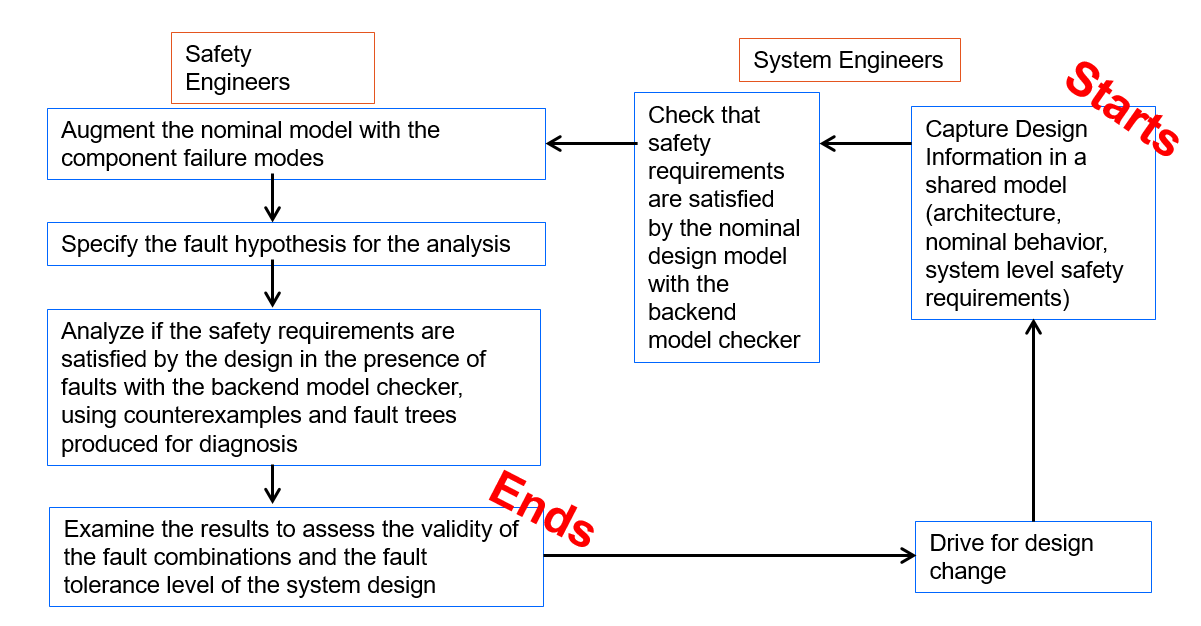
\includegraphics[width=\textwidth]{images/SACycle.PNG}
	\end{center}
	\caption{Proposed Steps of the Safety Assessment Process}
	\label{fig:SACycle1}
\end{figure}

These steps can be viewed as a cyclical process that involves both the system development engineers and the safety engineers of the system. Figure~\ref{fig:SACycle1} shows these steps within the context of the start and end of a project. 

\danielle{Add a bit more information here - pull from the MBSE project for IRAD. Include reasons why this approach is better, how it will help safety analysts, how it benefits the field as a whole. Then lead into the next sections with a statement about model checking, verification, etc.}

	%\section{Formal Methods}
\label{sec:fm}
As the complexity of systems increase, the cost of development and validation consumes more time and resources than ever before; nevertheless, these processes are vital in safety critical systems when the loss of functionality of the system can result in loss of life. Authorities have put in place various thresholds for the likelihood of such events and it is the responsibility of the system developers to show that undesirable events are sufficiently unlikely to occur~\cite{faaSA}. Utilizing the recent advancements in automated formal verification within the validation process has become essential to the certification of critical systems~\cite{deptOfDefense,standard1999,prasad2005survey} and the world of safety analysis began to see its powerful benefits~\cite{hinchey2012industrial, liggesmeyer1998improving, coudert1993fault, Bozzano:2010:DSA:1951720,bozzano2003esacs}. There arose multiple ways of viewing the system and fault models, various ways of automating the capture of safety pertinent information, and a number of tools that addressed practical issues. Formal validation and verification is a proof-based methodology used to assess the correctness of requirements, system design, and implementation. This section provides a background of the formal method techniques that are commonly used in the system development and safety assessment processes.

\subsection{Overview}
Given that this research is focused on model-based system development and safety assessment, we focus our attention onto \emph{model checking} as a method of formal analysis. Model checking is an automatic technique for verifying that system models meet their specified requirements~\cite{clarke2018model}.  Applying model checking to a system design consists of a few main tasks: \emph{modeling}, \emph{formal specification}, and \emph{formal verification}. The digital and mechanical components of a system can be described in abstract form (modeling), and the requirements of the system and of each component can be specified in formal logic (formal specification). Formal verification is demonstrating that the model satisfies its specification using math. The verification of a model takes both the design and the requirement specification into account when analyzing the behavior and interactions of the components. In the sections that follow, we will outline these three major components of model checking and describe the aspects important in this research.

\subsection{Modeling}
\label{sec:modeling}
When modeling a system, the digital and mechanical components are described in abstract form; furthermore, the requirements of the system and of each component can be specified in formal logic. The verification of such models take both the architecture and the requirement specification into account when analyzing the behavior and interactions of the components comprising the system. Throughout the past few decades, numerous modeling languages and tools have been introduced, for example Simulink from MathWorks~\cite{MathWorks}, SCADE from Esterel Technologies~\cite{abdulla2004designing}, and research base languages such as Lustre~\cite{Halbwachs91:IEEE}. Other common modeling languages include SysML~\cite{friedenthal2014practical} and AADL~\cite{FeilerModelBasedEngineering2012}. 

Often, engineers who design safety critical systems model their systems as networks of operators transforming flows of data. At a higher level, this can be represented by block diagrams that group these networks into reusable components. {\em Dataflow} languages allow these models to directly represent the digital control system. Dataflow programming languages have several merits, one of which is that the program is a completely functional model of the system. This feature makes the model well suited to formal verification and program transformation; it also facilitates reuse, because the module will behave the same way in any context into which it is embedded~\cite{joshi2008behavioral}. For this dissertation, we focus our attention on Lustre~\cite{Halbwachs91:IEEE}, a synchronous\footnote{A synchronous language breaks real time into a sequence of instants in which the outputs of the model are computed.} dataflow programming language used in the formal verification portion of this research. Lustre is described in more detail in Section~\ref{sec:lustre}. 




\begin{comment}
\subsubsection{Ordered Binary Decision Diagrams}
A Binary Decision Diagram (BDD) is a data structure used to encode Boolean formulae.
\begin{figure}[htbp]
        \center{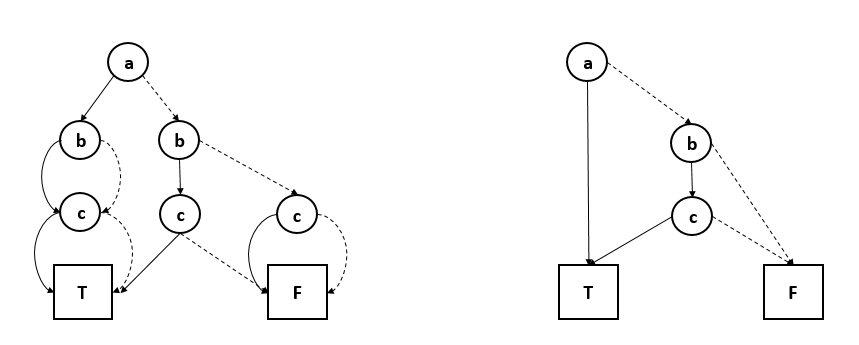
\includegraphics[width=0.8\textwidth] {images/bdd.png}}
        \caption{\label{fig:bdd} Binary Decision Diagrams of the Formula $a \lor (b \land c)$}
\end{figure}
As shown in Figure~\ref{fig:bdd}, it is a rooted, directed, acyclic graph with internal decision nodes and two terminal nodes (\textit{true} and \textit{false}). Each of the decision nodes is labeled with a Boolean variable and has two child nodes, low child and high child. The edge from a node to its low child represents the assignment of \textit{false}, likewise the edge to the high child represents the assignment of \textit{true}. The BDD is called \textit{ordered} if different variables appear in the same order on all paths from the root. Intuitively, following a path from the root to the \textit{true} terminal node represents a valid assignment to the Boolean formula (invalid in the case of ending on the \textit{false} terminal node). 

BDDs are reduced by the removal of isomorphic subgraphs. The BDD shown on the right of Figure~\ref{fig:bdd} is the reduced form of the BDD on the left.
\end{comment}


\subsection{Formal Specification}
\label{sec:formalSpec}
Before we can verify the correctness of a system, we must first specify the properties that the system should have~\cite{clarke2018model}. The formal specification process translates the informal system requirements into a mathematical logic to determine if the system design is correct~\cite{hinchey2012industrial}. This process guarantees an unambiguous description of the requirements, which is not possible when using an informal natural language. The formal definition of system requirements includes the system design and its expected behavior as well as the assumptions on the environment in which the system is expected to operate. A design or implementation can never be considered correct in isolation; it is only correct with respect to the specifications. The expected behavior, system design, and environmental assumptions change and are refined as the system goes through the various stages of development~\cite{lamsweerde2000formal}. A commonly used method of specification is \emph{temporal logic}. Temporal logics are useful for specifying complex system requirementss, because they can describe the ordering of events in time without introducing time explicitly. 

\subsubsection{Linear Temporal Logic}
Temporal logic can be used to express properties of reactive systems~\cite{Bozzano:2010:DSA:1951720}. System properties are usually classified into two main categories: {\em safety properties} and {\em liveness properties}. Safety properties express the idea that ``nothing bad ever happens" where liveness properties state that ``something good will eventually happen." 

An example of a safety property is: ``it is never the case that the brake pedal is pressed and no hydraulic pressure is supplied at the wheel." A liveness property, on the other hand, could state: ``eventually the process will complete its execution." 

Traditionally, two types of temporal logic are used in model checking; Computational Tree Logic (CTL), which is based on a branching time logic model, and Linear Temporal Logic (LTL), based on a linear representation of time. This research will focus on LTL. 

An LTL formula is built from a set of atomic propositions, logical operators, and basic temporal operators. The formula is evaluated over a linear path or sequence of states, $s_0, s_1, ..., s_i ,s_{i+1},...$. The following temporal operators are provided:
\begin{itemize}
    \item Globally (\textbf{G}): $G_p$ is true in a state $s_i$ if and only if $p$ is true in all states $s_j$ with $j \geq i$.
    
    \item Finally (\textbf{F}): $F_p$ is true in state $s_i$ if and only if $p$ is true in some state $s_j$ with $j \geq i$.
    
    \item Next (\textbf{X}): $X_p$ is true in state $s_i$ if and only if $p$ is true in the state $s_{i+1}$. 
    
    \item Until (\textbf{U}): $pUq$ is true in state $s_i$ if and only if $q$ is true in some state $s_j$ with $j \geq i$ and $p$ is true in all states $s_k$ such that $i \leq k < j$.
\end{itemize}

Other temporal operators can be defined on the basis of the operators above~\cite{sistla1985complexity}. Formal definitions and more information on LTL and CTL can be found in a number of research works~\cite{Bozzano:2010:DSA:1951720, clarke2018model}.

\subsection{Formal Verification} 
\label{sec:formalVer}
Once we have specified the important properties (formal specification), then a formal model for the system is created; this model captures the properties that must be considered to establish correctness~\cite{clarke2018model}; this process is referred in this dissertation as \emph{formal verification}. Formal verification is the use of proof methods to show that given the environmental assumptions stated in the formal specification, the formal design of the system meets the requirements. The problem can be reduced to that of property checking: given a program $P$ and a specific property, does the program satisfy the given property~\cite{fitting2012first}.  

Model checking was introduced in the early 1980s and consists of exploring the states and transitions of a model~\cite{clarke1981design,queille1982specification}. By representing the system abstractly, a possibly infinite state space is reduced to a finite model.~\cite{d2008survey}. The proofs are generated over an abstract mathematical model of the system, such as finite state machines, labeled transition systems, or timed automata. It takes as input a model of a system and the properties written in formal logic, then explores the state space of the system to determine if the model violates the properties~\cite{clarke2018model,fraser2009testing}. In recent years, model checking takes advantage of abstraction techniques specific to a domain to consider multiple states or transitions in a single operation; this lessens computation time considerably~\cite{d2008survey}. Nevertheless, the biggest limiting factor of model checking is scalability and much of the recent research in this area attempts to address this problem~\cite{clarke2018model}.

Deductive methods of verification consists of generating proof obligations from the specifications of the system and using these obligations in a theorem prover setting. Automated theorem provers have the main objective to show that some statement (conjecture) is a logical consequence of other statements (the axioms and hypotheses). The rules of inference are given as are the set of axioms and hypotheses~\cite{d2008survey,fitting2012first}. Deductive methods of verification include automated theorem provers (e.g., Coq~\cite{coq}, Isabelle~\cite{isabelle}) and satisfiability modulo theories (e.g., SMTInterpol~\cite{smtInterpol}, Z3~\cite{z3}, Yices~\cite{yices}). 



		%\subsection{Modeling}
\label{sec:modeling}
When modeling a system, the digital and mechanical components are described in abstract form; furthermore, the requirements of the system and of each component can be specified in formal logic. The verification of such models take both the architecture and the requirement specification into account when analyzing the behavior and interactions of the components comprising the system. Throughout the past few decades, numerous modeling languages and tools have been introduced, for example Simulink from MathWorks~\cite{MathWorks}, SCADE from Esterel Technologies~\cite{abdulla2004designing}, and research base languages such as Lustre~\cite{Halbwachs91:IEEE}. Other common modeling languages include SysML~\cite{friedenthal2014practical} and AADL~\cite{FeilerModelBasedEngineering2012}. 

Often, engineers who design safety critical systems model their systems as networks of operators transforming flows of data. At a higher level, this can be represented by block diagrams that group these networks into reusable components. {\em Dataflow} languages allow these models to directly represent the digital control system. Dataflow programming languages have several merits, one of which is that the program is a completely functional model of the system. This feature makes the model well suited to formal verification and program transformation; it also facilitates reuse, because the module will behave the same way in any context into which it is embedded~\cite{joshi2008behavioral}. For this dissertation, we focus our attention on Lustre~\cite{Halbwachs91:IEEE}, a synchronous\footnote{A synchronous language breaks real time into a sequence of instants in which the outputs of the model are computed.} dataflow programming language used in the formal verification portion of this research. Lustre is described in more detail in Section~\ref{sec:lustre}. 




\begin{comment}
\subsubsection{Ordered Binary Decision Diagrams}
A Binary Decision Diagram (BDD) is a data structure used to encode Boolean formulae.
\begin{figure}[htbp]
        \center{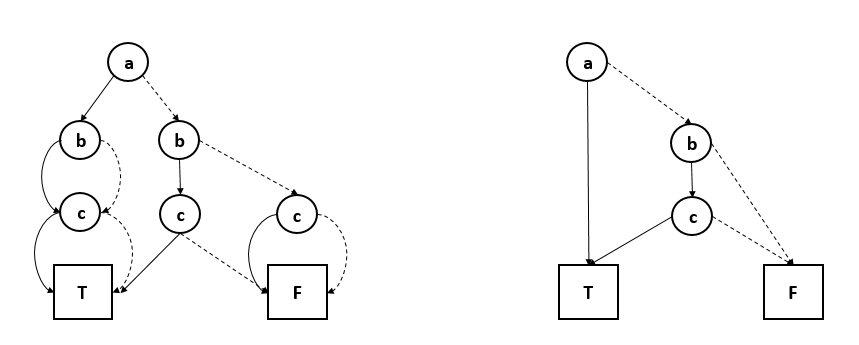
\includegraphics[width=0.8\textwidth] {images/bdd.png}}
        \caption{\label{fig:bdd} Binary Decision Diagrams of the Formula $a \lor (b \land c)$}
\end{figure}
As shown in Figure~\ref{fig:bdd}, it is a rooted, directed, acyclic graph with internal decision nodes and two terminal nodes (\textit{true} and \textit{false}). Each of the decision nodes is labeled with a Boolean variable and has two child nodes, low child and high child. The edge from a node to its low child represents the assignment of \textit{false}, likewise the edge to the high child represents the assignment of \textit{true}. The BDD is called \textit{ordered} if different variables appear in the same order on all paths from the root. Intuitively, following a path from the root to the \textit{true} terminal node represents a valid assignment to the Boolean formula (invalid in the case of ending on the \textit{false} terminal node). 

BDDs are reduced by the removal of isomorphic subgraphs. The BDD shown on the right of Figure~\ref{fig:bdd} is the reduced form of the BDD on the left.
\end{comment} % TS
		%\input{modelchecking} %ltl, etc
		%\subsubsection{The SAT Problem and SMT Solvers}
\label{sec:satsmt}
The Boolean Satisfiability (SAT) problem attempts to determine if there exists a total truth assignment to a given propositional formula, that evaluates to $true$. Generally, a propositional formula is any combination of the disjunction and conjunction of literals (as an example, $a$ and $\neg a$ are literals). For example, the proposition $a \land b$ is satisfiable; when $a$ and $b$ are assigned to $true$, the formula is satisfied, or true.  On the other hand, the proposition $a \land \neg a$ is unsatisfiable; no such assignment can be found to satisfy both $a$ and $\neg a$. 

Satisfiability Modulo Theories (SMT) solvers also address the SAT problem, but can work over propositional logic or predicate logic with quantifiers. An SMT solver works over a conjunction of literals, as is the case with SAT solvers, but the literals can be expressed as predicates over non-boolean variables, such as $x > 0$. A boolean literal can be satisfied with a finite number of possible assignments; this is not always the case with an SMT formula.


\textbf{UNSAT Cores and Minimal Unsatisfiable Subsets}
When analyzing a model, there are certain questions that may be asked about the model requirements. If a model is unsatisfiable with respect to some system level property, it is of benefit to know \emph{why} it is not satisfiable. 

A constraint system $C$ is an ordered set of $n$ abstract constraints $\{C_1, C_2, ..., C_n\}$ over a set of variables. The constraint $C_i$ restricts the allowed assignments of these variables in some way~\cite{liffiton2016fast}. Given a constraint system, we require some method of determining, for any subset $S \subseteq C$, whether $S$ is \textit{satisfiable} (SAT) or \textit{unsatisfiable} (UNSAT). Given a constraint system $C$, there are certain subsets of $C$ that are of interest in terms of satisfiability. Definitions 2-4 are taken from research by Liffiton et. al.~\cite{liffiton2016fast}. 

For a given unsatisfiable problem, SAT solvers (and SMT solvers) attempt to provide proof of unsatisfiability by providing a subset of UNSAT clauses known as \textit{UNSAT cores}. In general, this is useful information to have regarding the constraint system in question. 

\begin{definition} A Minimal Unsatisfiable Subset (MUS) $M$ of a finite constraint system $C$ is a subset $M \subseteq C$ such that $M$ is unsatisfiable and $\forall c \in M$ : $M \setminus \{c\}$ is satisfiable. 
\end{definition}

\begin{definition} UNSAT core: Let $C$ be a finite set of constraints and $U \subseteq C$ an unsatisfiable subset. A constraint $c \in U$ is an UNSAT core for $U$ if $U \setminus \{c\}$ is satisfiable. A set of all unsatisfiability cores of $U$ constitute an MUS for $C$. 
\end{definition}

Intuitively, an MUS is the minimal explanation of the constraint systems infeasability and the UNSAT cores are the building blocks of the MUS. In recent years, a number of efficient algorithms have been introduced to find MUSs~\cite{liffiton2005max} and most of them focus on finding a single such subset~\cite{belov2012towards, belov2013core, belov2012muser2}. More recently, algorithms have been introduced that can find all such minimal unsatisfiable subsets~\cite{GhassabaniGW16, Ghassabani2017EfficientGO,bendik2018online}. 


\textbf{Inductive Validity Cores} Given a complex model, it is useful to extract traceability information related to the proof; in other words, which elements of the model were necessary to construct the proof of a safety property. An algorithm was introduced by Ghassabani et al. to provide Inductive Validity Cores (IVC) as a way to determine which model elements are necessary for the inductive proofs of the safety properties for sequential systems~\cite{GhassabaniGW16}. Given a safety property of the system, a model checker is invoked to construct a proof of the property. The IVC generation algorithm extracts traceability information from the proof process and returns a minimal set of the model elements required in order to prove the property. Later research extended this algorithm in order to produce all minimal IVC elements (\aivcalg)~\cite{Ghassabani2017EfficientGO,bendik2018online}. 

The \aivcalg algorithm considers a constraint system consisting of the assumptions and contracts of system components and the negation of the safety property of interest (i.e. the top level event). It then collects all Minimal Unsatisfiable Subsets (MUSs) of this constraint system; these are the minimal explanations of the constraint systems infeasibility in terms of the \textit{negation} of the safety property. Equivalently, these are the minimal model elements necessary to prove the safety property. 

 

		%\subsection{Compositional Model Checking and AGREE}
\label{compModelChecking}
Compositional analysis of systems was introduced in order to address the scalability of model checking large software systems~\cite{pnueli1985transition, heckel1998compositional, NFM2012:CoGaMiWhLaLu}. Normally, a SAT solver will flatten the hierarchical system model and use all model elements from all layers in order to find proof of a safety property. The analysis can alternatively be performed compositionally following the architecture hierarchy such that analysis at a higher level is based on the components at the next lower level and conducted layer by layer; the components of a system are organized hierarchically and each layer of the architecture is viewed a system. The idea is to partition the formal analysis of a system architecture into verification tasks that correspond into the decomposition of the architecture. 

\subsubsection{Assume-Guarantee Reasoning Environment}
The Assume-Guarantee Reasoning Environment (AGREE)~\cite{cofer2012compositional} provides a way to perform compositional verification on models that are defined using the Architecture Analysis and Design Language (AADL)~\cite{aerospace2012sae}. 

A component contract in an assume-guarantee reasoning environment is an assume-guarantee pair. Intuitively, the meaning of a pair is: if the assumption is true, then the component will ensure that the guarantee is true. The formulation of AGREE uses LTL operators $G$ (globally), $H$ (historically), and $Z$ (in the previous instant).

Formally, a component contract is an assume-guarantee pair $(A,P)$ for propositions $A, P$. The meaning of a pair is that a component is required to meet it's guarantee only if its assumptions have been true up to the current instant~\cite{cofer2012compositional}. Stated as an LTL formula, this is $G(H(A) \implies P)$. 

Each architectural layer is viewed as a system with inputs, outputs, and components. A system $S$ can be described as its own contract $(A_S, P_S)$ and the contracts of its components $C_S$. Thus, $S = (A_S, P_S, C_S)$. For each layer, the proof consists of demonstrating that the system guarantee is provable given the guarantees of its direct subcomponents and the system assumptions, or more formally prove $G(H(A_S) \implies P_S)$ given $G(H(A_C) \implies P_C)$ for each component $C$ in the system.  

This proof is performed one layer at a time starting from the top level of the system. When compared to monolithic analysis (i.e., analysis of the flattened model composed of all components), the compositional approach allows the analysis to scale to much larger systems~\cite{NFM2012:CoGaMiWhLaLu}. AGREE utilizes the JKind model checker~\cite{2017arXiv171201222G}, an infinite state $k$-induction model checker. Verification of the program is performed using a back-end SMT solver, e.g., Z3~\cite{z3}, SMTInterpol~\cite{smtInterpol}. 

	%\section{Formal Methods in Safety Analysis: A Brief History and the State of the Practice}
\label{sec:modelCheckingInSA}
Safety analysis has traditionally been performed manually, but with the rise of model checking and the improvement of its capabilities, the world of safety analysis began to see its powerful benefits~\cite{hinchey2012industrial, liggesmeyer1998improving, coudert1993fault, Bozzano:2010:DSA:1951720,bozzano2003esacs}. There arose multiple ways of viewing the system and fault models, various ways of automating the capture of safety pertinent information, and a number of tools that addressed various issues that arose. In this section, we discuss the state of the practice of related work and how formal methods has been applied in the domain of safety assessment research.

\subsection{Model Checking in Model Based Safety Analysis}
From the beginnings of model checking, there was a slow increase in its application to the domain of safety analysis, but a few research groups contributed immensely to this branch of study. Separately, these researchers began to contribute to safety analysis through the use of formal methods in the '90s and are still contributing today (e.g., \cite{reese1997software,signoret1998altarica,chiappini1999formal,cimatti2000industrial}. 

One of the main methods was the abstraction of the system into a formal transition system; this provided a means of defining a precise mathematical model of the system and simplifying mathematical operations through the use of abstraction techniques on the transition system. This helped to shrink the entire state space into something more digestible by computational techniques~\cite{d2008survey}. 

In the early 2000s, model based safety assessment began to make an appearance in literature~\cite{Bozzano:2010:DSA:1951720,Joshi05:Dasc, Joshi05:SafeComp, Joshi07:Hase}. The researchers began applied model checking in model based system development to safety analysis.  In this approach, a safety analysis system model is the central artifact in the safety analysis process, and traditional safety analysis artifacts, such as fault trees, are automatically generated by tools that analyze the system model.

The contents and structure of the safety analysis system model differ significantly across different conceptions of model-based safety analysis.  We can draw distinctions between approaches along several different axes.  The first is whether they propagate errors explicitly through user-defined propagations, which we call {\em explicit propagation}, or through behavioral requirements and interactions in the model itself, which we call {\em implicit propagation}.  The next is whether models and notations are {\em purpose-built} for safety analysis vs. those that extend {\em existing system models}.

For implicit propagation approaches, there are several additional dimensions.  One dimension involves whether {\em causal} or {\em non-causal} models are allowed.  Non-causal models allow simultaneous (in time) bi-directional error propagations, which allow more natural expression of some failure types (e.g. reverse flow within segments of a pipe), but are more difficult to analyze.  A final dimension involves whether analysis is {\em compositional} across layers of hierarchically-composed systems or {\em monolithic}.  

\begin{figure}[h]
	\begin{center}
		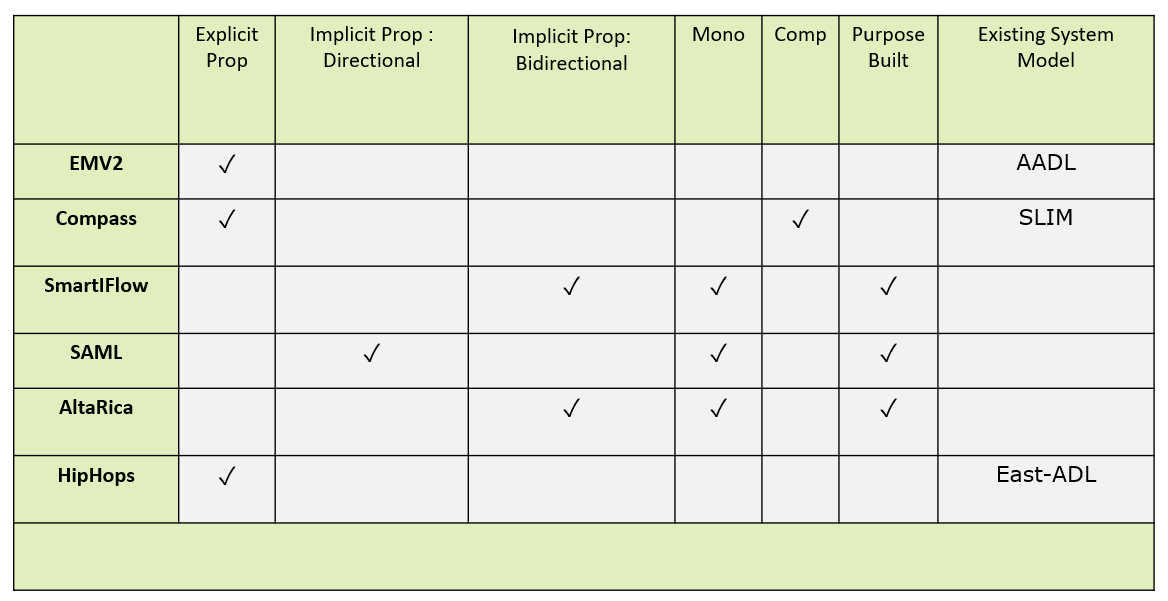
\includegraphics[width=\textwidth]{images/relatedWork.PNG}
	\end{center}
	\caption{Approaches of Related Work}
	\label{fig:relatedWork}
\end{figure}

Figure~\ref{fig:relatedWork} highlights the differences between these approaches in closely related work. The left column of the figure shows the tool names and across the top row are the various ways of structuring and analyzing the safety analysis system model. The tools and their approaches are described in the following subsections. 

These tools attempt to address various needs in the safety community and do so in distinct ways, but we wish to combine many of these efforts under one existing system model. We make it possible to extend the AADL system model with a fault model. Both nominal and fault analysis should be able to be performed monolithically or compositionally, and the fault model should allow for either explicit or implicit propagation. We attempt to address multiple needs within a single framework, unlike many of the related tools. 

This literature overview is not a complete account of all safety analysis model checking tools available either in industry or research, but highlights some of the most influential safety assessment methods and tools currently available. 

\subsubsection{AltaRica}
AltaRica was one of the first model checking tools specifically aimed at safety analysis of critical systems. The first iteration of AltaRica (1.0) performed over a transition system of the model, used dataflow ({\em causal}) semantics, and could capture the hierarchy of a system~\cite{signoret1998altarica}. The key idea was that this transition system (more specifically {\em constraint automata}) could be compiled into Boolean formulae and transformed into a binary decision diagram~\cite{point1999altarica}. The literature for performing fault tree analysis over BDDs was rich with algorithms; this was how much of the safety analysis artifacts were generated. The dataflow dialect (AltaRica 1.0) has substantial tool support, including the commercial Cecilia OCAS tool from Dassault~\cite{bieber2004safety}. For this dialect, the safety assessment, fault tree generation, and functional verification can be performed with the aid of NuSMV model checking~\cite{symbAltaRica}.

The most recent language update (AltaRica 3.0) uses non-causal semantics~\cite{prosvirnova2013compilationfaulttrees,prosvirnova2015automated,PROSVIRNOVA2013127}. Failure states are defined throughout the system and flow variables are updated through the use of assertions~\cite{Bieber04safetyassessment}.  AltaRica 3.0 has support for simulation and Markov model generation through the OpenAltaRica (www.openaltarica.fr) tool suite; it uses {\em implicit error propagation}, and it is a {\em purpose-built}, {\em monolithic} safety analysis language. 

\subsubsection{FSAP, xSAP, and COMPASS}
The Formal Safety Analysis Platform (FSAP) was introduced in 2003~\cite{bozzano2003improving} and supported failure mode definitions, safety requirements in temporal logic formulae, automated fault tree construction, and counterexample traces. The platform used NuSMV, a binary decision diagram (BDD)-based model checker~\cite{Cimatti2000}. The system model, written in NuSMV, and the fault model, developed graphically in FSAP, are together translated into a finite state machine and eventually into a BDD; fault tree analysis is performed using BDD algorithms implemented in NuSMV. 

By 2016, the researchers that developed FSAP (Foundation Bruno Kessler, FBK) released a similar tool called xSAP~\cite{DBLP:conf/tacas/BittnerBCCGGMMZ16}. xSAP extends FSAP in many ways: xSAP can handle infinite state machines, it is textual language rather than graphical, allows for richer fault modeling and definitions, and implements more than just BDD computations (e.g., SAT- and SMT-based routines). xSAP was integrated into the COMPASS toolsuite to take advantage of the algorithms it supports. More complex SAT-based algorithms were introduced to bypass the BDD method of minimal cut set generation, namely the ``anytime approximation" algorithms~\cite{CAV2015:BoCiGrMa, mattarei2016scalable}. These algorithms make clever use of bounded model checking algorithms to explore counterexamples provided to the query "the top level event never occurs." These explorations are done such that the cut sets generated are of increasing cardinality which allows for an approximation computation to be given even when the state space is too large to compute all minimal cut sets. These are implemented in xSAP~\cite{CAV2015:BoCiGrMa}.

COMPASS (Correctness, Modeling project and Performance of Aerospace Systems)~\cite{10.1007/978-3-642-04468-7_15} allows for {\em explicit propagation}, and is a {\em causal} {\em compositional} tool suite that uses the SLIM language, which is based on a subset of the Architecture Analysis and Design Language (AADL), for its input models~\cite{5185388, criticalembeddedsystems}. In SLIM, a nominal system model and the error model are developed separately and then transformed into an extended system model.  This extended model is automatically translated into input models for the NuSMV model checker~\cite{Cimatti2000, NuSMV}, MRMC (Markov Reward Model Checker)~\cite{Katoen:2005:MRM:1114692.1115230, MRMC}, and RAT (Requirements Analysis Tool)~\cite{RAT}. The safety analysis tool xSAP~\cite{DBLP:conf/tacas/BittnerBCCGGMMZ16} can be invoked in order to generate safety analysis artifacts such as fault trees and FMEA tables~\cite{compass30toolset}.  %COMPASS is an impressive tool suite, but some of the features that make AADL suitable for SW/HW architecture specification: event and event-data ports, threads, and processes, appear to be missing, which means that the SLIM language may not be suitable as a general system design notation (ESM).

\subsubsection{SmartIFlow}
SmartIFlow~\cite{info17:HaLuHo,honig2014new} uses {\em implicit propagation} and is a {\em purpose-built}, {\em monolithic} {\em non-causal} safety analysis tool that describes components and their interactions using finite state machines and events. Verification is done through an explicit state model checker which returns sets of counterexamples for safety requirements in the presence of failures.  SmartIFlow allows {\em non-causal} models containing simultaneous (in time) bi-directional error propagations.  On the other hand, the tools do not yet appear to scale to industrial-sized problems, as mentioned by the authors: ``As current experience is based on models with limited size, there is still a long way to go to make this approach ready for application in an industrial context''~\cite{info17:HaLuHo}.

\subsubsection{SAML}
The Safety Analysis and Modeling Language (SAML)~\cite{Gudemann:2010:FQQ:1909626.1909813} uses {\em implicit propagation}, and is a {\em purpose-built}, {\em monolithic} {\em causal} safety analysis language that was developed in 2010.  System models constructed in SAML can be used used for both qualitative and quantitative analyses. It allows for the combination of discrete probability distributions and non-determinism. The SAML model can be automatically imported into several analysis tools like NuSMV~\cite{Cimatti2000}, PRISM (Probabilistic Symbolic Model Checker)~\cite{CAV2011:KwNoPa}, or the MRMC model checker~\cite{Katoen:2005:MRM:1114692.1115230}. SAML itself does not provide the formal verification engines, but instead provides a platform to model the safety aspects of a system and then translate this into the input language for a formal verification engine~\cite{Gudemann:2010:FQQ:1909626.1909813}.

\subsubsection{Error Model Annex for AADL}
The SAE (Society of Automotive Engineers) released the
aerospace standard AS5506, named Architecture Analysis and Design Language (AADL), which is a mature industry-standard for embedded systems and has proved to be efficient for architecture modeling~\cite{aerospace2012sae,liu2016research}. AADL supports safety analysis by adding EMA (Error Model Annex) as an extension to the language. EMA allows the user to annotate system hardware and software architectures with hazard, error propagation, failure modes and effects due to failures. Around 2016, Version 2 of the Error Model Annex was released (EMV2)~\cite{EMV2}. EMV2 uses {\em explicit propagation} and is based on an {\em existing system model} approach. The faults and error propagations are explicitly defined and the fault tree analysis is performed by traversing propagation paths in reverse to find the original fault that caused the problem~\cite{feiler2017automated}. 


 % related work

\chapter{Fault Modeling and the Safety Annex}
\label{chap:faultModeling}
Early on in Section 2.2.1, a model-based safety assessment process was proposed. This process was backed by formal methods and incorporates a shared model into the development and safety analysis processes. A high level description of this cyclical process is shown in Figure~\ref{fig:SACycle} for your convenience. 

\begin{figure}[h]
	\begin{center}
		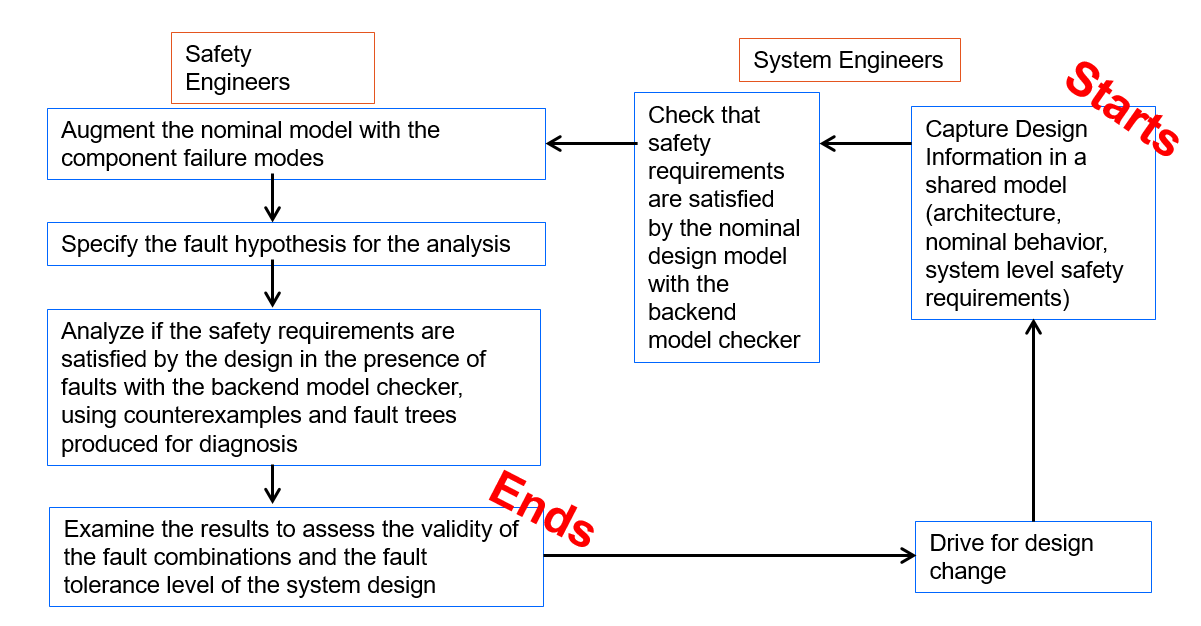
\includegraphics[width=\textwidth]{images/SACycle.PNG}
	\end{center}
	\caption{Proposed Steps of the Safety Assessment Process}
	\label{fig:SACycle}
\end{figure}

There are certain capabilities that are required in order to fully perform all steps of this process. In beginning this research, we outlined what those pieces were and investigated related work to determine if a gap still existed. Based on the related work summary found in Section 2.7, it is clear that this work fills certain gaps that no previous research has addressed:

\begin{description}[nosep]

    \item[Shared model] using a language expressive enough to describe HW and SW components.
    \item[Flexible error propagations] through both behavioral and explicit means.
    \item[Flexible fault modeling] with support for a/symmetric faults, in/dependent faults, etc.
    \item[Model checker] used to assess and verify the design with or without faults active.
    \item[Ability to generate artifacts] used in the safety assessment process.
\end{description}

In previous chapters, we discussed how a model checker can be used to generate minimal cut sets in a compositional fashion. In this chapter, the fault modeling process using the Safety Annex for the Architecture Analysis and Design Language (AADL)~\cite{AADL_Standard} is described. The Safety Annex was developed with these two broad ideas in mind: (1) how this supports the proposed safety assessment process, and (2) what missing pieces need to be addressed in order to support safety analysts. 

\section{Fault, Failure, and Error Terminology}
The usage of the terms error, failure, and fault are defined in ARP4754A and are described here for ease of understanding~\cite{SAE:ARP4754A}. An \textit{error} is a mistake made in implementation, design, or requirements. A \textit{fault} is the manifestation of an error and a \textit{failure} is an event that occurs when the delivered service of a system deviates from correct behavior. If a fault is activated under the right circumstances, that fault can lead to a failure. The terminology used in the Error Model Annex version 2 for AADL (EMV2)~\cite{EMV2}, differs slightly for an error: an error is a corrupted state caused by a fault. The error propagates through a system and can manifest as a failure. In this dissertation, we use the ARP4754A terminology with the added definition of \textit{error propagation} as used in EMV2. An error is a mistake made in design or code and an error propagation is the propagation of the corrupted state caused by an active fault. 

\section{Implementation of the Safety Annex}
The Safety Annex is written in Java as a plug-in for the OSATE AADL toolset, which is built on Eclipse.  It is not designed as a stand-alone extension of the language, but works with behavioral contracts specified using the AGREE annex for AADL~\cite{NFM2012:CoGaMiWhLaLu}. 
The architecture of the Safety Annex is shown in Figure~\ref{fig:plugin-arch}.

\begin{figure}[h]
	\begin{center}
		%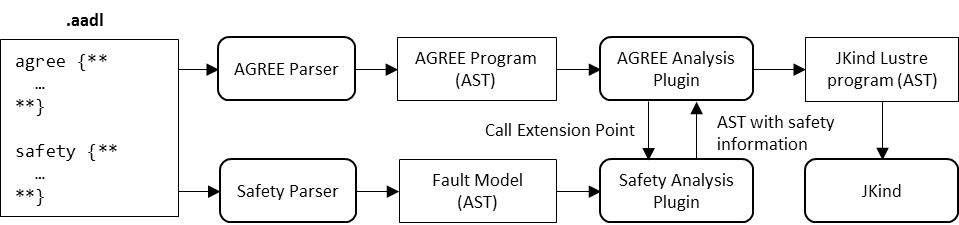
\includegraphics[trim=0 400 430 0,clip,width=0.85\textwidth]{images/arch.png}
		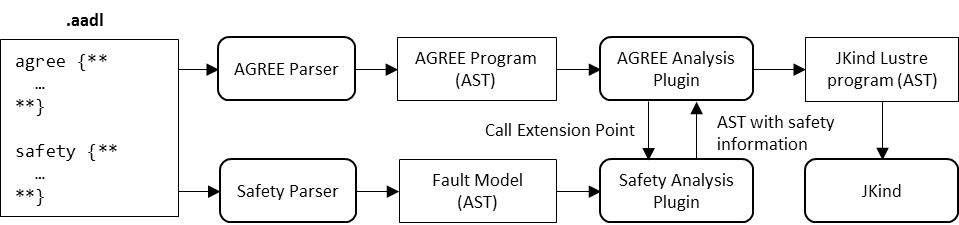
\includegraphics[width=\textwidth]{images/arch.png}
	\end{center}
	%\vspace{-0.2in}
	\caption{Safety Annex Plug-in Architecture}
	\label{fig:plugin-arch}
	%\vspace{-0.2in}
\end{figure}

AGREE contracts are used to define the nominal behaviors of system components as {\em guarantees} that hold when {\em assumptions} about the values the component's environment are met. When an AADL model is annotated with AGREE contracts and the fault model is created using the Safety Annex, the model is transformed through AGREE into a Lustre model~\cite{Halbwachs91:IEEE} containing the behavioral extensions defined in the AGREE contracts for each system component. 

When performing fault analysis, the Safety Annex extends the AGREE contracts to allow faults to modify the behavior of component inputs and outputs. An example of a portion of an initial AGREE node and its extended contract is shown in Figure~\ref{fig:lustre}. The left column of the figure shows the nominal Lustre pump definition is shown with an AGREE contract on the output; and the right column shows the additional local variables for the fault (boxes 1 and 2), the assertion binding the fault value to the nominal value (boxes 3 and 4), and the fault node definition (box 5). Once augmented with fault information, the AGREE model (translated into the Lustre dataflow language~\cite{Halbwachs91:IEEE}) follows the standard translation path to the model checker JKind~\cite{2017arXiv171201222G}, an infinite-state model checker for safety properties. 

\begin{figure}[h!]
	%\hspace*{-2cm}
	%\vspace{-0.3in} 
	\begin{center}
		%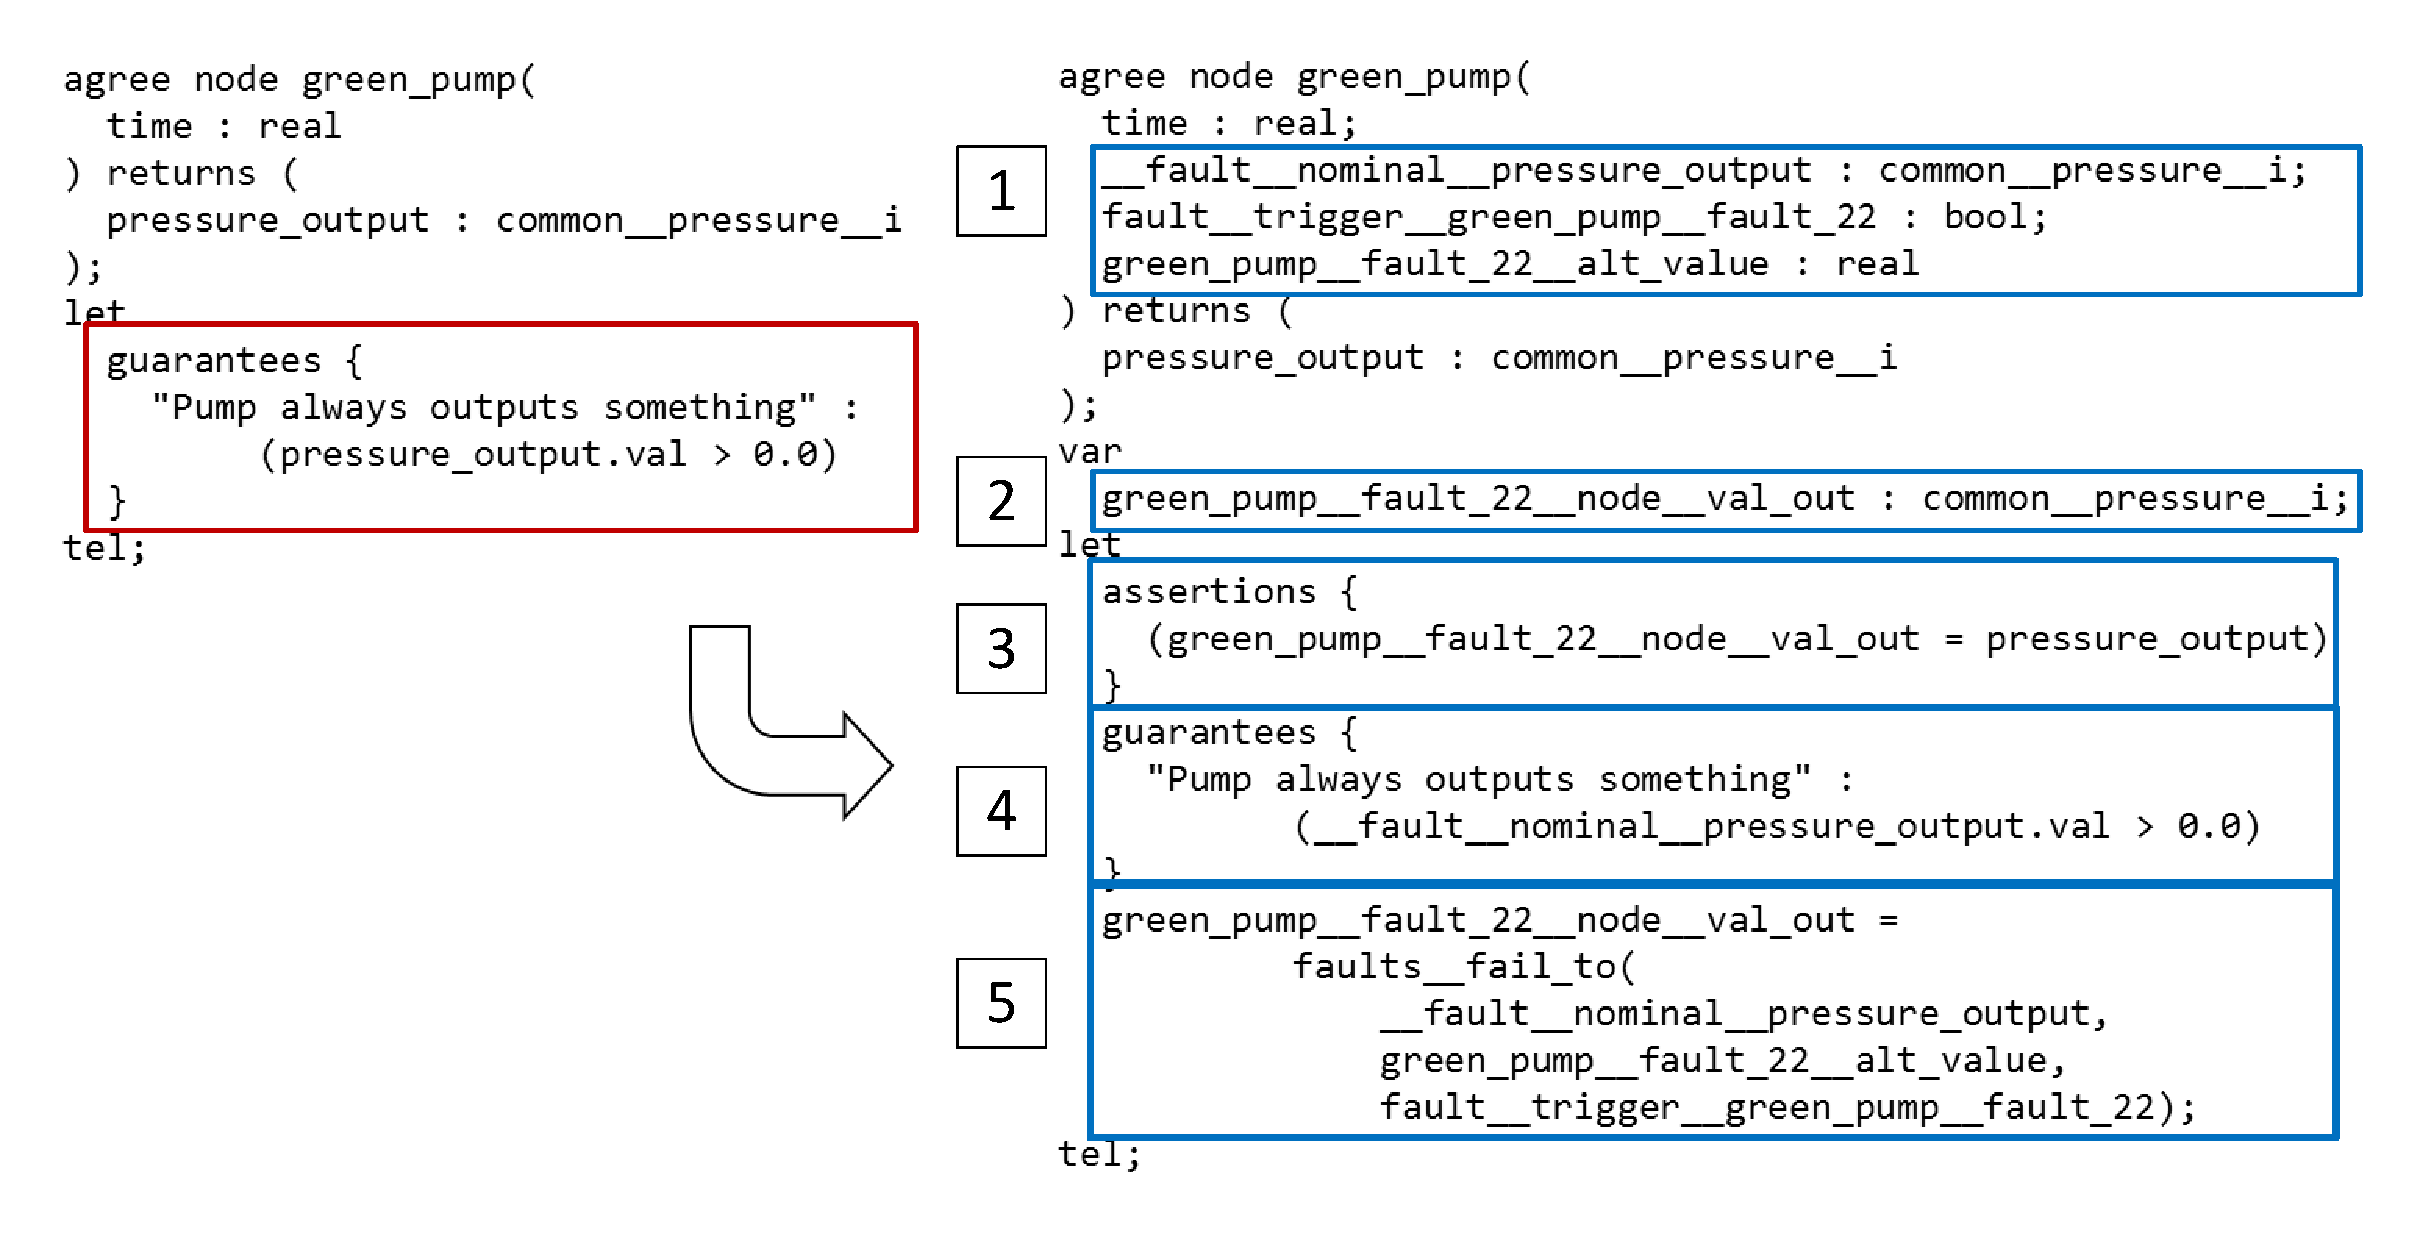
\includegraphics[trim=0 690 -10 70,clip,width=1.5\dimexpr\textwidth-2cm\relax]{images/lustre.pdf}
		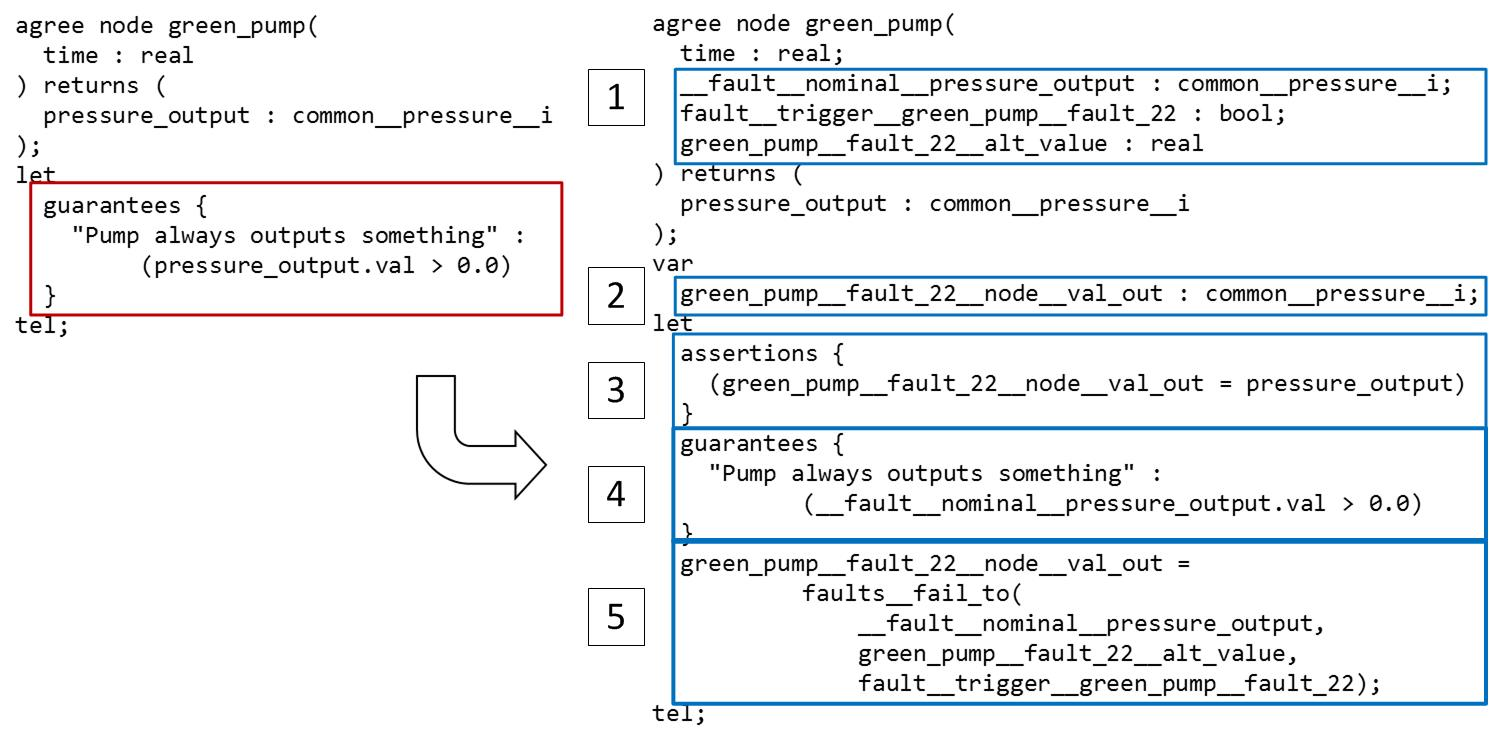
\includegraphics[scale=0.3]{images/lustre.jpg}
		%\caption{Nominal AGREE node and its extension with faults}
		\caption{Nominal AGREE Node and Extension with Faults}
		\label{fig:lustre}
	\end{center}
	%\vspace{-0.3in}
\end{figure}

There are two different types of fault analysis that can be performed on a fault model. The Safety Annex plugin intercepts the AGREE program and add fault model information to the model depending on which form of fault analysis is being run.

\textbf{Verification in the Presence of Faults}: This analysis returns one counterexample when fault activation per the fault hypothesis can cause violation of a property. The augmentation from Safety Annex to the AGREE program includes traceability information so that when counterexamples are displayed to users, the active faults for each component are visualized.

\textbf{Generate Minimal Cut Sets}: This analysis collects all minimal set of fault combinations that can cause violation of a property. As described in Chapter~\ref{chap:mcsGen}, the first step of MinCutSet generation is to collect the minimal IVCs for each property. Given the compositional nature of the verification, each level of the system is extended in a slightly different way. The leaf nodes of a system contribute only constrained faults to the \aivcalg algorithm as shown in Figure~\ref{fig:ivcElements1}. 

\begin{figure}[h!]
	\hspace*{-2cm}
	\vspace{-0.1in} 
	\begin{center}
		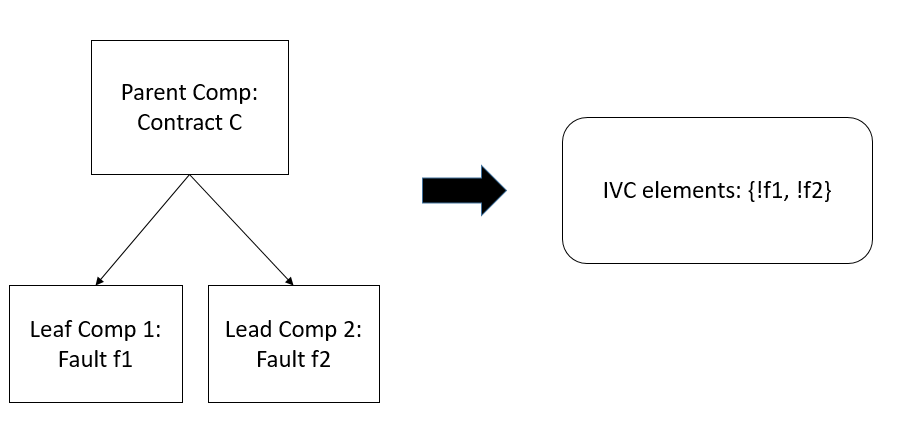
\includegraphics[scale=0.5]{images/ivcElements1.png}
	\caption{IVC Elements used for Consideration in a Leaf Layer of a System}
		\label{fig:ivcElements1}
	\end{center}
\end{figure}

In the non-leaf layers of the program, both contracts and constrained faults are considered as shown in Figure~\ref{fig:ivcElements2}. The reason for this is that the contracts are used to prove the properties at the next highest level and are necessary for the verification of the properties. 

\begin{figure}[h!]
	\hspace*{-2cm}
	\vspace{-0.1in} 
	\begin{center}
		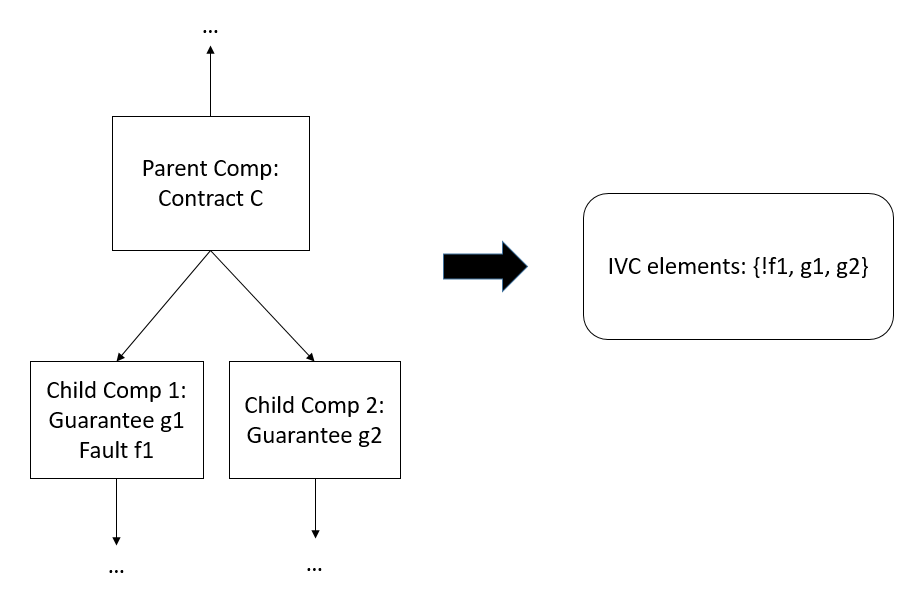
\includegraphics[scale=0.5]{images/ivcElements2.png}
	\caption{IVC Elements used for Consideration in a Middle Layer of a System}
		\label{fig:ivcElements2}
	\end{center}
\end{figure}

The \aivcalg algorithm returns the minimal set of these elements necessary to prove the properties. This equates to any contracts or inactive faults that must be present in order for the verification of properties in the model. From here, we transform all MIVCs into minimal cut sets.


\section{Component Fault Modeling}
The Safety Annex is used to add possible faulty behaviors to a component model. Within the AADL component instance model, an annex is added which contain the fault definitions for the given component. The flexibility of the fault definitions allows the user to define numerous types of fault \textit{nodes} by utilizing the AGREE node syntax. %A library of common fault nodes has been written and is available in the project GitHub repository~\cite{SAGithub}. 
Examples of such faults include valves being stuck open or closed, output of a software component being nondeterministic, or power being cut off.  When the fault analysis requires fault definitions that are more complex, these nodes can easily be written and used in the model. 

When a fault is activated by its specified triggering conditions, it modifies the output of the component. This faulty behavior may violate the contracts of other components in the system, including assumptions of downstream components. The impact of a fault is computed by the AGREE model checker when the safety analysis is run on the fault model. 

The majority of faults that are connected to outputs of components are known as \textit{symmetric}. That is, whatever components receive this faulty output will receive the same faulty output value. Thus, this output is seen symmetrically. An alternative fault type is \textit{asymmetric}. This pertains to a component with a 1-n output: one output which is sent to many receiving components. This fault can present itself differently to the receiving components. For instance, in a boolean setting, one component might see a true value and the rest may see false. This is also possible to model using the keyword \textit{asymmetric}. For more details on fault definitions and fault modeling capabilities, we refer readers to the Safety Annex Users Guide\cite{SAGithub}.

\danielle{Need to either explain the example here or use a different example than WBS. WBS is used A LOT in this section, so perhaps a short description is okay...}
As an illustration of fault modeling using the Safety Annex, we look at one of the components important to the inadvertent braking property: the brake pedal. When the mechanical pedal is pressed, a sensor reads this information and passes an electronic signal to the BSCU which then commands hydraulic pressure to the wheels. 

%Figure~\ref{fig:sensor} 
Figure~\ref{fig:sensor} shows the AADL pedal sensor component with a contract for its nominal behavior. The sensor has only one input, the mechanical pedal position, and one output, the electrical pedal position. 
A property that governs the behavior of the component is that the mechanical position should always equal the electronic position. (The expression \textit{true $\rightarrow$ property} in AGREE is true in the initial state and then afterwards it is only true if property holds.)

\begin{figure}[h!]
	\hspace*{-2cm}
	%\vspace{-0.55in} 
	\begin{center}
		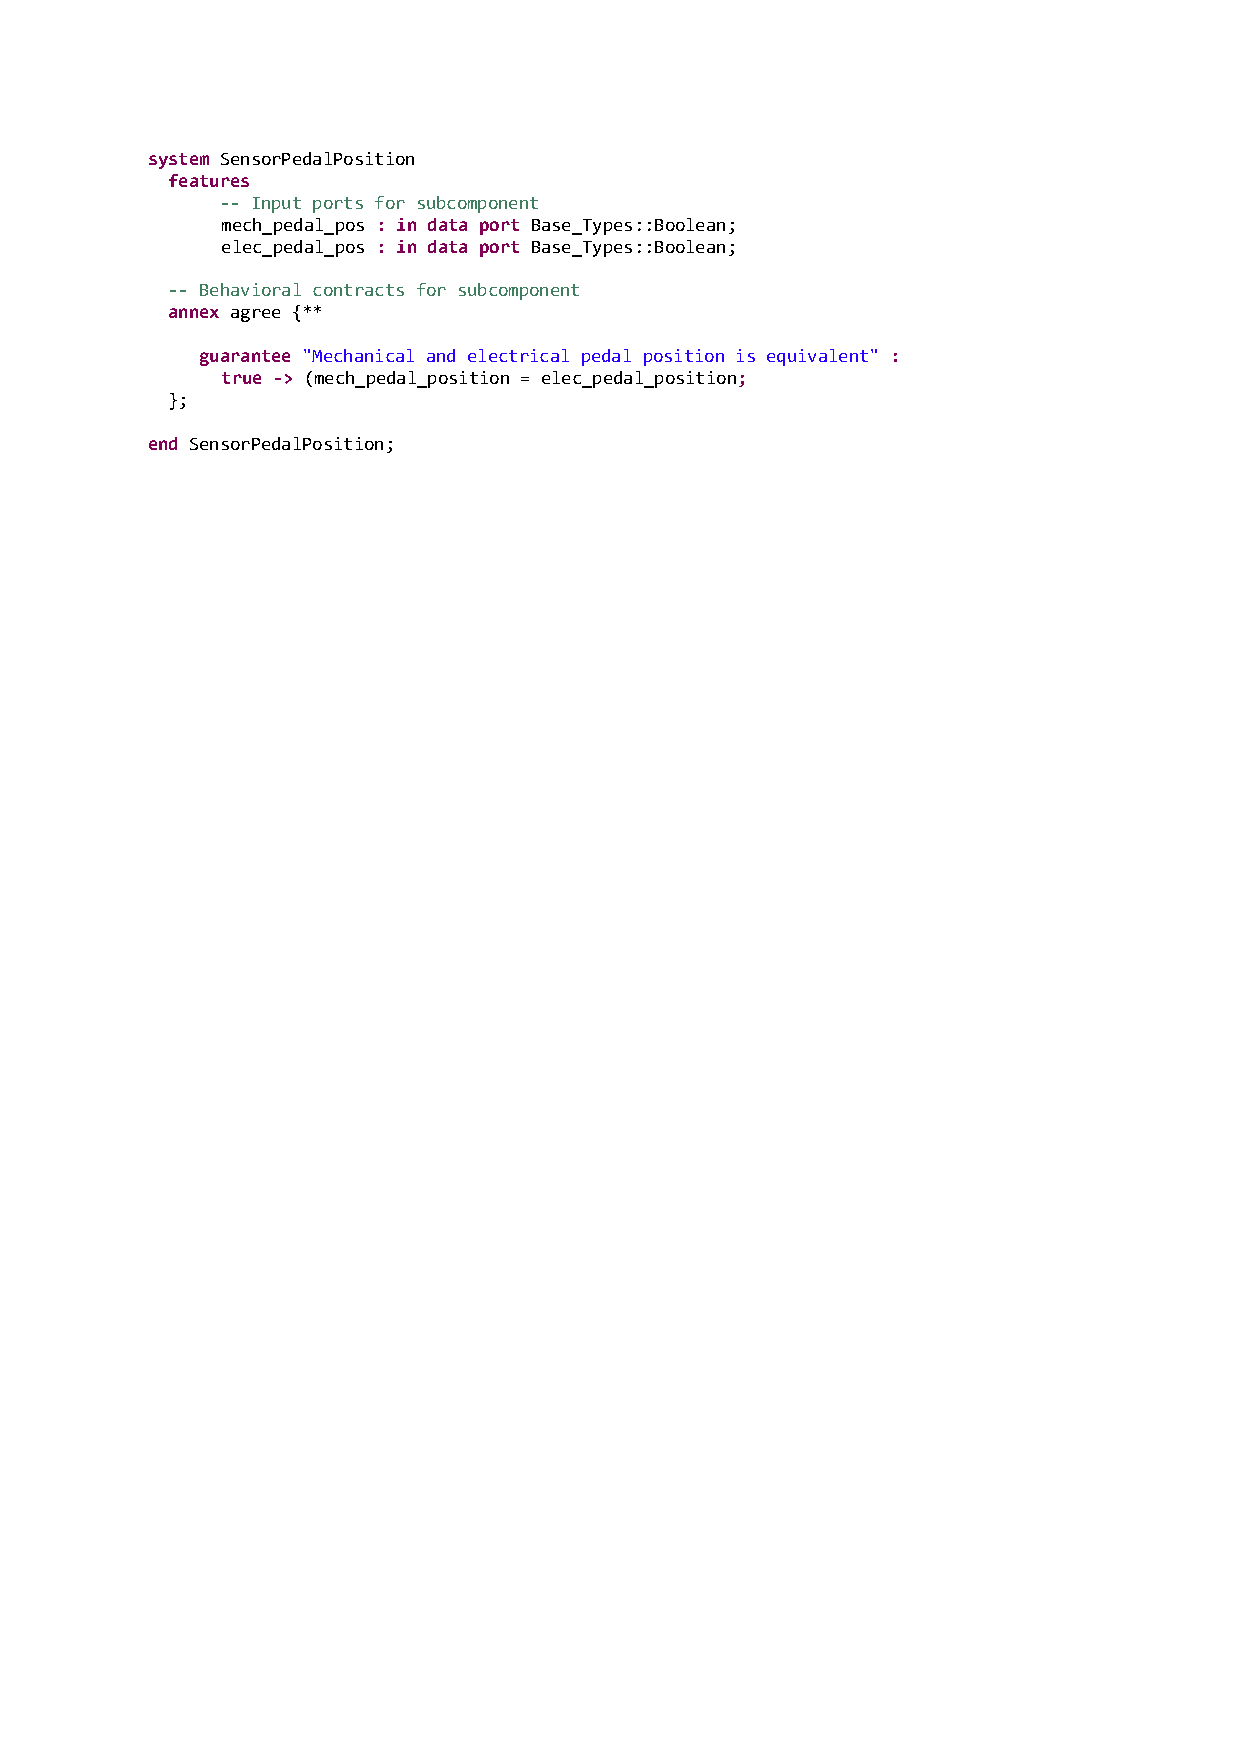
\includegraphics[trim=0 640 -10 70,clip,width=1.5\dimexpr\textwidth-2cm\relax]{images/system_sensor.pdf}
		\vspace{-0.3in}
		\caption{An AADL System Type: The Pedal Sensor}
		\label{fig:sensor}
	\end{center}
	\vspace{-0.2in}
\end{figure}

One possible failure for this sensor is inversion of its output value. This fault can be triggered with probability $5.0\times 10^{-6}$ as described in AIR6110 (in reality, the component failure probability is 
collected from hardware specification sheets).  
The Safety Annex definition for this fault is shown in Figure~\ref{fig:sensorFault}. Fault behavior is defined through the use of a fault node called \textit{inverted\_fail}.  When the fault is triggered, the nominal output of the component (\textit{elec\_pedal\_position}) is replaced with its failure value (\textit{val\_out}). 

\begin{figure}[h!]
	\hspace*{-2cm}
	%\vspace{-0.5in} 
	\begin{center}
		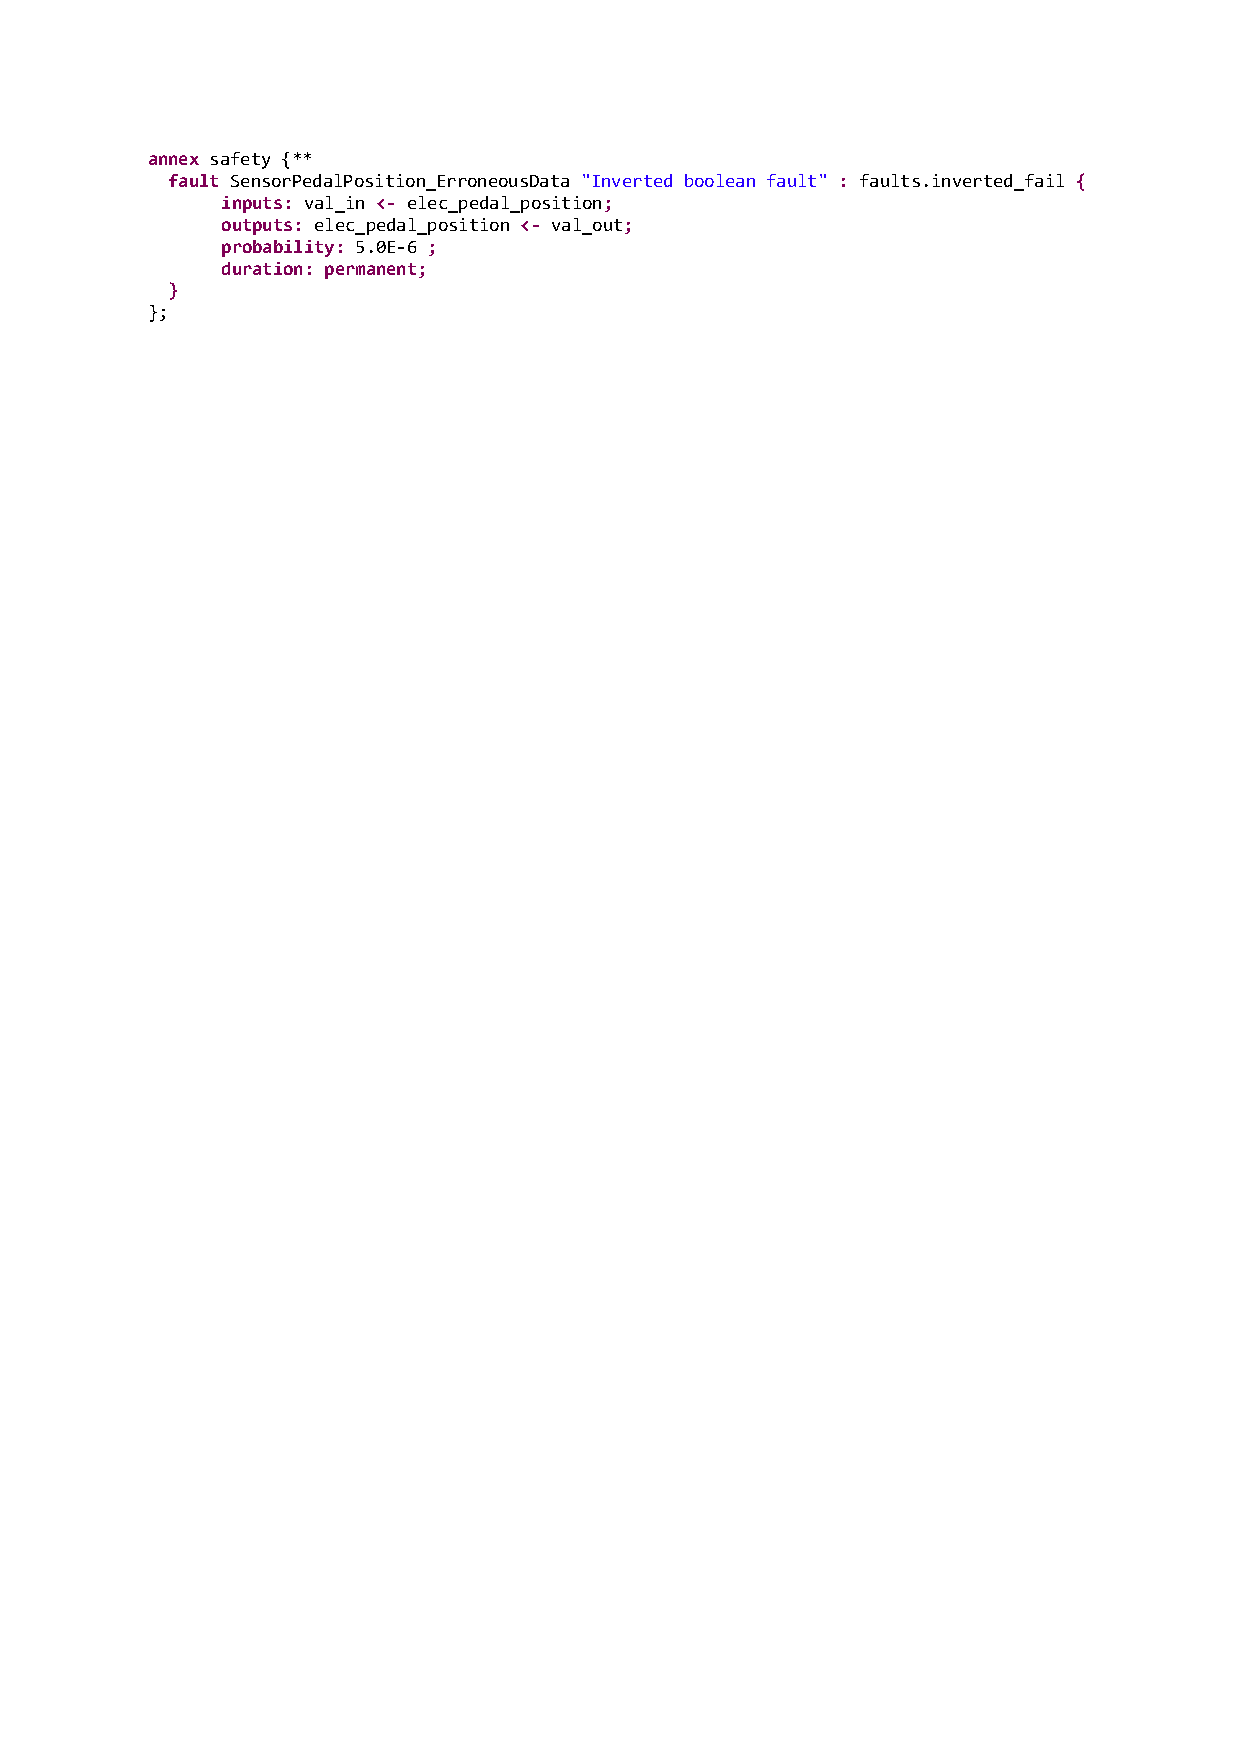
\includegraphics[trim=0 680 -10 70,clip,width=1.5\dimexpr\textwidth-2cm\relax]{images/safetyannex_sensorfault.pdf}
		\vspace{-0.2in}
		\caption{The Safety Annex for the Pedal Sensor}
		\label{fig:sensorFault}
	\end{center}
	\vspace{-0.2in}
\end{figure}

The WBS fault model expressed in the Safety Annex contains a total of 33 different fault types and 141 fault instances. The large number of fault instances is due to the redundancy in the system design and its replication to control 8 wheels.

\section{Error Propagation}
As systems become larger and more complex, it can be difficult knowing all possible error propagations within a model; using a purely explicit approach to error propagation is difficult. To this end, we developed the Safety Annex to primarily use \textit{behavioral} propagation. In this approach, the faults are attached to a component's output and ``turned on" in a manner of speaking. The effects and propagation of the active fault is revealed through the behavioral contracts of the system by use of the model checker. 

This section outlines the Safety Annex approach to implicit error propagation and also describes how one can model an explicit propagation by defining dependent faults. 

\subsection{Implicit Propagation}
In the Safety Annex approach, faults are captured as faulty behaviors that augment the system behavioral model in AGREE contracts. No explicit %fault
error propagation is necessary since the faulty behavior itself propagates through the system just as in the nominal system model. The effects of any triggered fault are manifested through analysis of the AGREE contracts. 

On the contrary, in the AADL Error Model Annex, Version 2 (EMV2)~\cite{EMV2} approach, all errors must be explicitly propagated through each component (by applying fault types on each of the output ports) in order for a component to have an impact on the rest of the system. To illustrate the key differences between implicit %failure
error propagation provided in the Safety Annex and the explicit %failure 
error propagation provided in EMV2, we use a simplified behavioral flow from the WBS example using code fragments from EMV2, AGREE, and the Safety Annex. 

\begin{figure}[h]
	%\hspace*{-2cm}
%	\vspace{-0.19in}
	\centering
	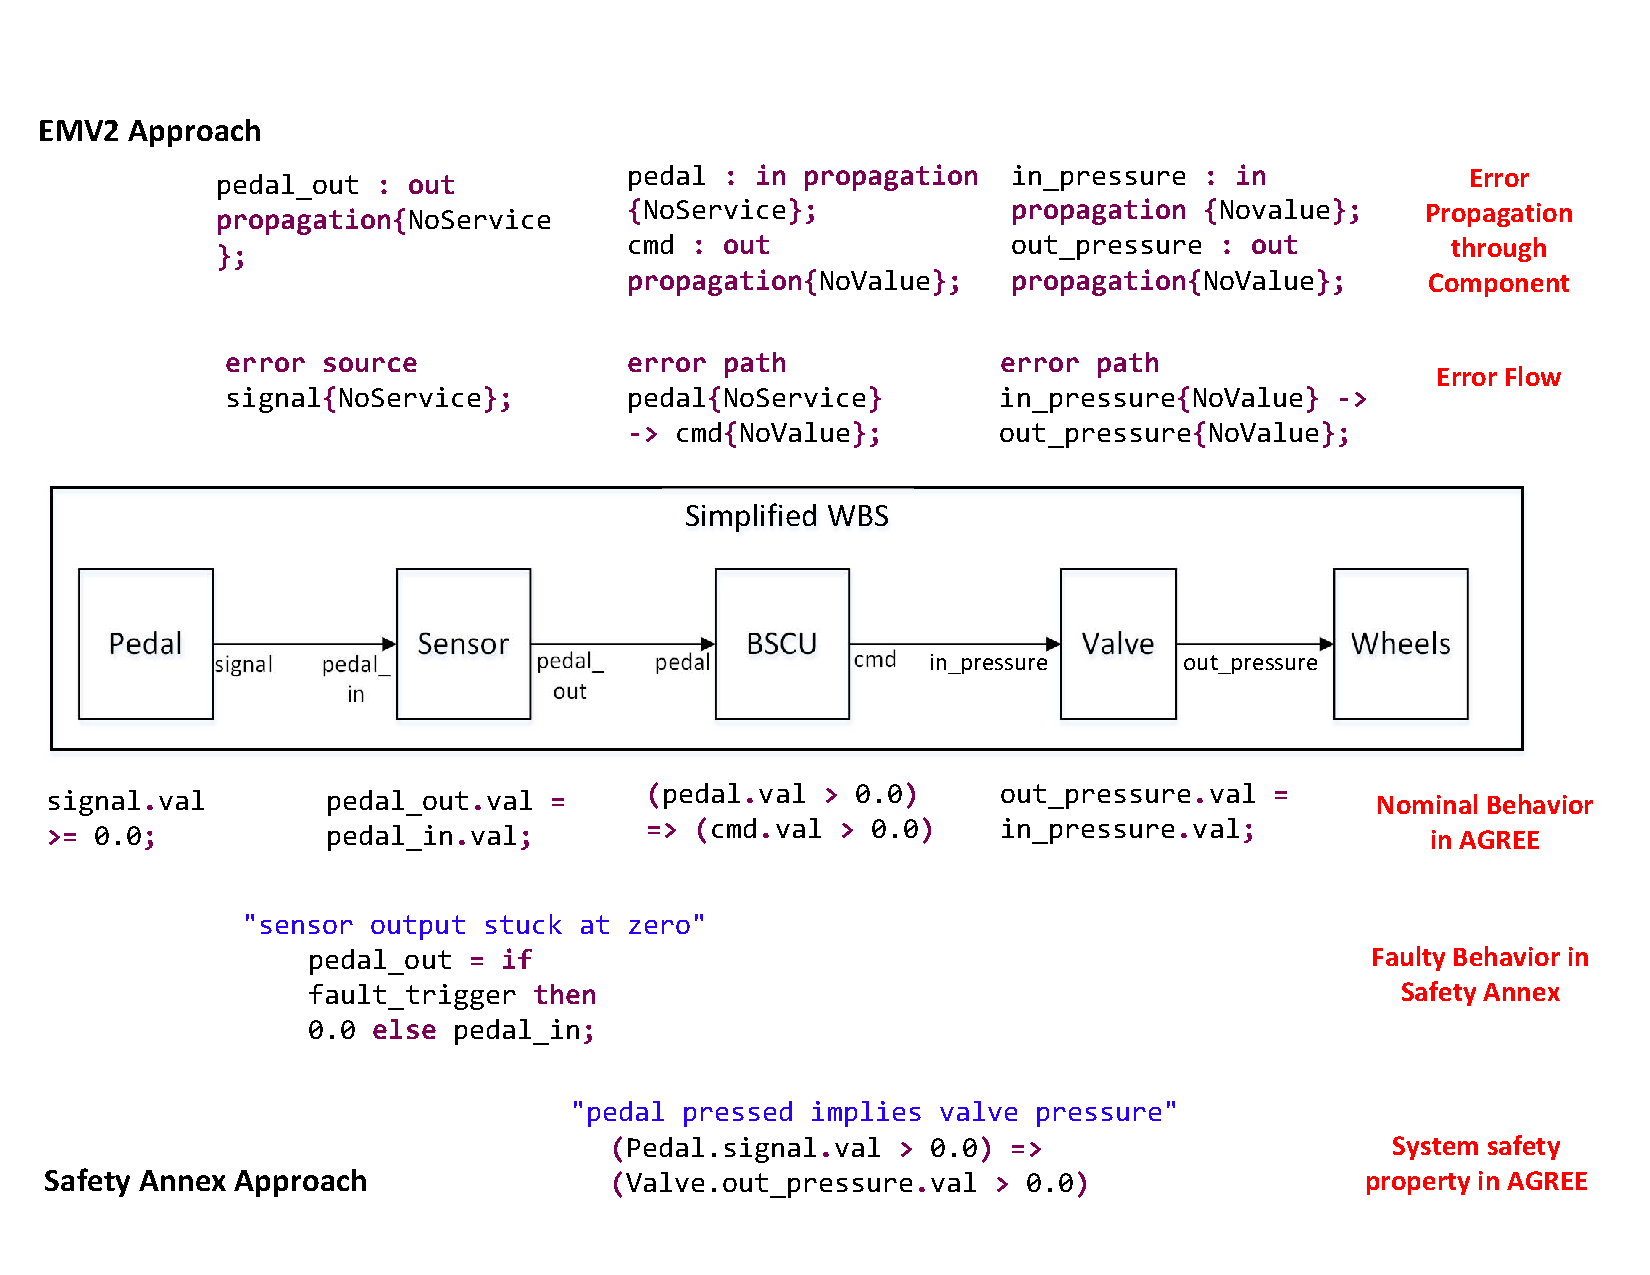
\includegraphics[trim=0 9 0 5,clip,width=\textwidth]{images/Comparison_with_EMV2.pdf}
	%\vspace{-0.3in}
	\caption{Differences between Safety Annex and EMV2}
	\label{fig:comparison_with_EMV2}
	%\vspace{-0.2in}
\end{figure} 

In this simplified WBS system, the physical signal from the Pedal component is detected by the Sensor and the pedal position value is passed to the Braking System Control Unit (BSCU) components.  The BSCU generates a pressure command to the Valve component which applies hydraulic brake pressure to the Wheels. 

In the EMV2 approach (top half of Figure~\ref{fig:comparison_with_EMV2}), the ``NoService'' fault is explicitly propagated through all of the components. These fault types are essentially tokens that do not capture any analyzable behavior. At the system level, analysis tools supporting the EMV2 annex can aggregate the propagation information from different components to compose an overall fault flow diagram or fault tree. 

When a fault is triggered in the Safety Annex (bottom half of Figure~\ref{fig:comparison_with_EMV2}), the output behavior of the Sensor component is modified. In this case the result is a ``stuck at zero'' error. The behavior of the BSCU receives a zero input and proceeds as if the pedal has not been pressed. This will cause the top level system contract to fail: {\em pedal pressed implies brake pressure output is positive}.


\subsection{Explicit Propagation} 
%Faults
Failures in hardware (HW) components can trigger behavioral faults in the system components that depend on them. For example, a CPU %fault
Failure may trigger faulty behavior in the threads bound to that CPU. In addition, a %fault
failure in one HW component may trigger %faults
failure in other HW components located nearby, such as overheating, fire, or explosion
in the containment location. 
The Safety Annex provides the capability to explicitly model the impact of hardware %faults
failures on other faults, behavioral or non behavioral. The explicit propagation to non behavioral faults is similar to that provided in EMV2.

To better model %HW dependent faults 
faults at the system level dependent on HW failures, a fault model element is introduced called a \textit{hardware fault}. Users are not required to specify behavioral effects for the HW faults, nor are data ports necessary on which to apply the fault definition. An example of a model component fault declaration is shown below:
\begin{figure}[h!]
	%\vspace{-0.1in}
	\begin{center}
	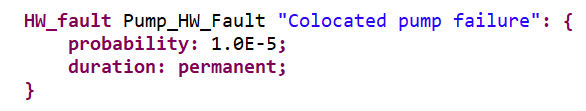
\includegraphics[width=.6\textwidth]{images/hw_fault2.png}
	\end{center}
	\vspace{-0.1in}
	\caption{Hardware Fault Definition}
	\label{fig:hwFault}
	%\vspace{-0.2in}
	%\vspace{-0.1in}
\end{figure}

Users specify dependencies between the HW component faults and faults that are defined in other components, either HW or SW. The hardware fault then acts as a trigger for dependent faults. This allows a simple propagation from the faulty HW component to the SW components that rely on it, affecting the behavior on the outputs of the affected SW components.

In the WBS example, assume that both the green and blue hydraulic pumps are located in the same compartment in the aircraft and an explosion in this compartment rendered both pumps inoperable. 
The HW fault definition can be modeled first in the green hydraulic pump component as shown in Figure~\ref{fig:hwFault}. The activation of this fault triggers the activation of related faults as seen in the \textit{propagate\_to} statement shown in Figure~\ref{fig:hwFaultProp}. 
Notice that these pumps need not be connected through a data port in order to specify this propagation. %Furthermore, the probability of the HW fault activation can be specified. 

\begin{figure}[h!]
	%\vspace{-0.1in}
	\begin{center}
		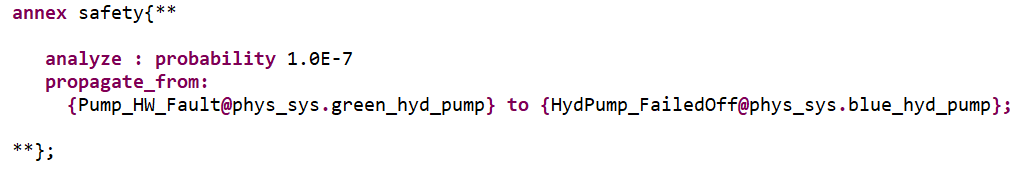
\includegraphics[width=1.0\textwidth]{images/hw_prop_stmt.png}
	\end{center}
	\vspace{-0.1in}
	\caption{Hardware Fault Propagation Statement}
	\label{fig:hwFaultProp}
	%\vspace{-0.2in}
	%\vspace{-0.1in}
\end{figure}

The fault dependencies are specified in the system implementation where the system configuration that causes the dependencies becomes clear (e.g., binding between SW and HW components, co-location of HW components). 
%This is because fault propagations are typically tied to the way components are connected or bound together; this information may not be available when faults are being specified for individual components. Having fault propagations specified outside of a component’s fault statements also makes it easier to reuse the component in different systems. 



\section{Fault Analysis Statements}
%An annotation in the AADL model determines the fault analysis statement (also referred to in this report as the fault hypothesis). This may specify either a maximum number of faults that can be active at any point in execution:
The fault analysis statement (also referred to as the fault hypothesis) resides in the AADL system implementation that is selected for verification. This may specify either a maximum number of faults that can be active at any point in execution:

\begin{figure}[h!]
	\vspace{-0.1in}
	%\begin{center}
		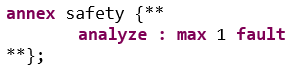
\includegraphics[width=0.4\textwidth]{images/hypothesisMaxN.png}
	%\end{center}
	\vspace{-0.1in}
	%%\caption{Max N Faults Analysis Statement}
	\label{fig:hypothesisMaxN}
\end{figure}
or that the only faults to be considered are those whose probability of simultaneous occurrence is above some probability threshold: 

\begin{figure}[h!]
	\vspace{-0.1in}
	%\begin{center}
		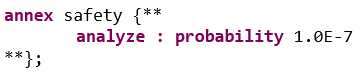
\includegraphics[width=0.5\textwidth]{images/hypothesisProb.png}
	%\end{center}
	\vspace{-0.1in}
	%\caption{Probability Analysis Statement}
	%\label{fig:hypothesisProb}
\end{figure}

Tying back to the fault tree analysis in traditional safety analysis, the former is analogous to restricting the cutsets to a specified maximum number of terms, and the latter is analogous to restricting the cutsets to only those whose probability is above some set value. In the former case, we assert that the sum of the true {\em fault\_\_trigger} variables is at or below some integer threshold.  In the latter, we determine all combinations of faults whose probabilities are above the specified probability threshold, and describe this as a proposition over {\em fault\_\_trigger} variables. 
%
With the introduction of dependent faults, active faults are divided into two categories: independently active (activated by its own triggering event) and dependently active (activated when the faults they depend on become active). The top level fault hypothesis applies to independently active faults. Faulty behaviors augment nominal behaviors whenever their corresponding faults are active (either independently active or dependently active).

\section{Asymmetric Fault Modeling}
\label{sec:byzantine}
A \textit{asymmetric} or \textit{Byzantine} fault is a fault that presents different symptoms to different observers~\cite{Driscoll-Byzantine-Fault}. In our modeling environment, asymmetric faults may be associated with a component that has a one-to-many ($1-n$) output to multiple ($n$) other components. In this configuration, a \textit{symmetric} fault will result in all destination components seeing the same faulty behavior from the source component. To capture the behavior of asymmetric faults (``different symptoms to different observers''), it was necessary to extend our fault modeling mechanism in AADL. A thorough description of the asymmetric modeling capability of the Safety Annex is shown in Chapter~\ref{chap:caseStudies} using a process ID example.

\subsection{Implementation of Asymmetric Faults}
To illustrate our implementation of asymmetric faults, assume a source component A has a 1-n output connected to four destination components (B-E) as shown in Figure~\ref{fig:commNodes} under ``Nominal System.'' If a symmetric fault was present on this output, all four connected components would see the same faulty behavior. An asymmetric fault should be able to present arbitrarily different values to the connected components. 

To this end, ``communication nodes'' are inserted on each connection from component A to components B, C, D, and E (shown in Figure~\ref{fig:commNodes} under ``Fault Model Architecture.'' From the users perspective, the asymmetric fault definition is associated with component A's output and the architecture of the model is unchanged from the nominal model architecture. Behind the scenes, these communication nodes are created to facilitate potentially different fault activations on each of these connections. The fault definition used on the output of component A will be inserted into each of these communication nodes as shown by the red circles at the communication node output in Figure~\ref{fig:commNodes}.
\begin{figure}[!htb]
        \center{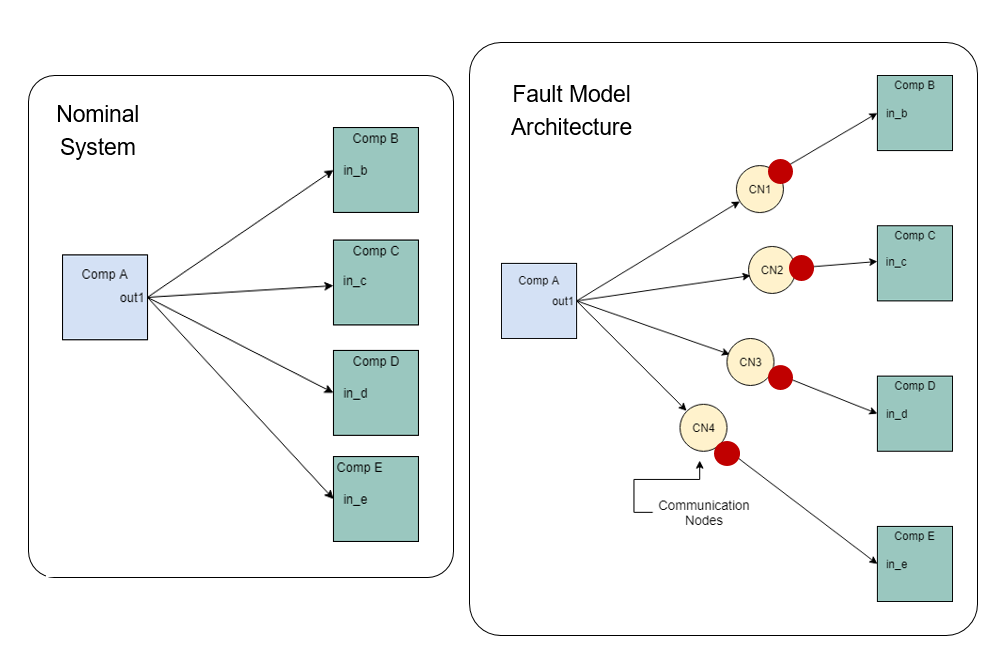
\includegraphics[width=\textwidth] {images/commNodes.png}}
        \caption{\label{fig:commNodes} Communication Nodes in Asymmetric Fault Implementation}
\end{figure}

\begin{figure}[!htb]
        \center{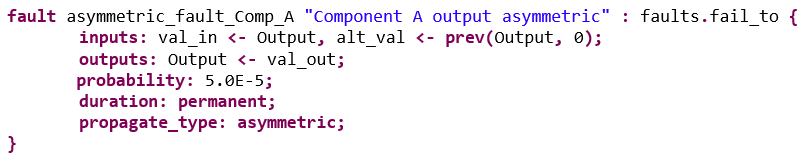
\includegraphics[width=\textwidth] {images/asymFaultDef.png}}
        \caption{\label{fig:asymFaultDef} Asymmetric Fault Definition in the Safety Annex}
\end{figure}

An asymmetric fault is defined for Component A as in Figure~\ref{fig:asymFaultDef}. This fault defines an asymmetric failure on Component A that when active, is stuck at a previous value (\textit{prev(Output, 0)}). This can be interpreted as the following: some connected components may only see the previous value of Comp A output and others may see the correct (current) value when the fault is active. This fault definition is injected into the communication nodes and which of the connected components see an incorrect value is completely nondeterministic. Any number of the communication node faults (0…all) may be active upon activation of the main asymmetric fault.

%\subsection{Referencing Fault Activation Status}
%To fully implement the agreement protocol, it must be possible to describe whether or not a subcomponent is failed by specifying if any faults defined for the subcomponents is activated. In the Safety Annex, this is made possible through the use of a \textit{fault activation} statement. Users can declare boolean \textit{eq} variables in the AGREE annex of the AADL system where the AGREE verification applies to that system's implementation. %in AGREE and in the implementations Safety Annex,  Users can then assign the activation status of specific faults to those \textit{eq} variables in Safety Annex of the AADL system implementation (the same place where the fault analysis statement resides).
%assigns this boolean \textit{eq} statement to a fault specific to a subcomponent.  This assignment links each specified AGREE boolean variable with the activation status of the specified fault activation literal. The AGREE boolean variable is true when and only when the fault is active. This additional feature of the Safety Annex allows users to state contracts of the form: if \texttt{sensor\_failed} then \texttt{do\_something}.

 










	%\input{byzantine}
	%\section{Implementation of the Safety Annex}
\label{sec:impl}
%Important features were considered before the implementation of the safety annex; these we addressed one by one and will outline below. 

As described in Section~\ref{sec:concepts}, an AADL~\cite{AADL_Standard} model describes a system in terms of a hierarchy of components and their interconnections, where each component can either represent a logical entity (e.g., application software functions, data) or a physical entity (e.g., buses, processors). AADL is used to specify and analyze real-time embedded systems. It includes specifications specific to hardware, software, and system component abstractions. The language definition is sufficiently rigorous to support formal analysis tools that allow for early phase error/fault detection~\cite{FeilerModelBasedEngineering2012}. 

\begin{figure}[h!]
	%\vspace{-0.1in}
	\begin{center}
	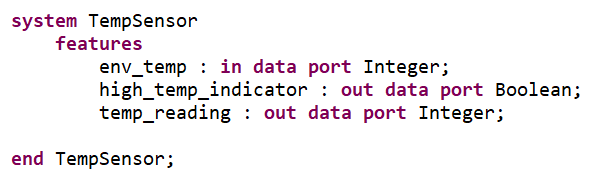
\includegraphics[width=.8\textwidth]{images/aadlComponent.png}
	\caption{AADL Component Types}
	\label{fig:aadlComponent}
	%\vspace{-0.2in}
	%\vspace{-0.1in}
	\end{center}
\end{figure}

Central to an AADL model are component \emph{types} and \emph{implementation} declarations. Figure~\ref{fig:aadlComponent} shows an example of a simple sensor component type defined in AADL. The component has an environmental temperature as input and two outputs: a high temperature indication and a temperature reading. In the type declaration, you define the category (\texttt{system} in this example) and features such as inputs and outputs; the implementation contains definitions of the internal structure of the component, e.g., internal constituents and their interactions. 

\begin{figure}[h!]
	%\vspace{-0.1in}
	\begin{center}
	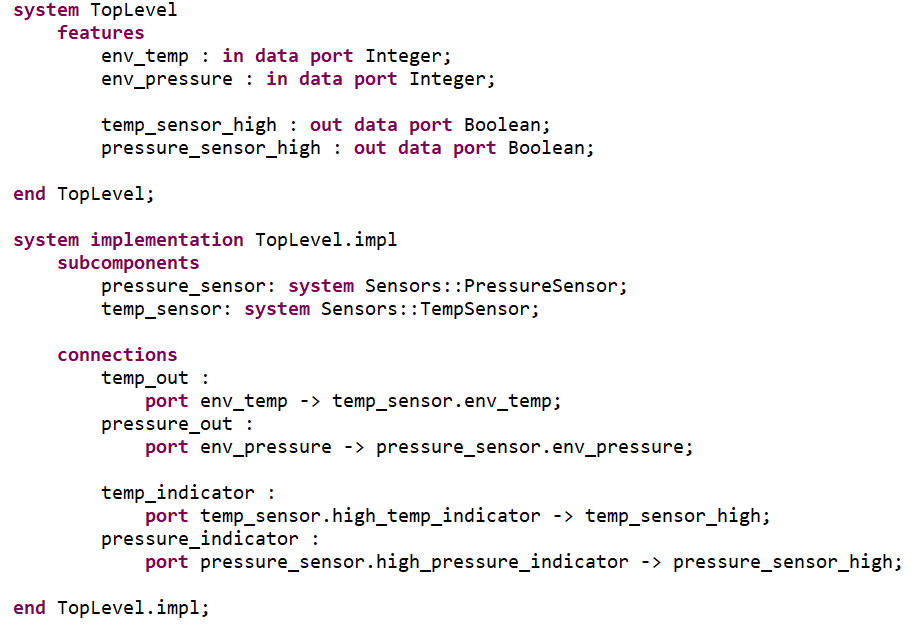
\includegraphics[width=1.0\textwidth]{images/aadlImplementation.png}
	\caption{An AADL Component Implementation Definition}
	\label{fig:aadlImplementation}
	%\vspace{-0.2in}
	%\vspace{-0.1in}
	\end{center}
\end{figure}

An implementation of the sensor component type is shown in Figure~\ref{fig:aadlImplementation}. The system contains a type of its own (top of figure: \texttt{system TopLevel}) which holds any environmental inputs or subcomponent outputs. The implementation defines the subcomponents of the system and their connections (bottom half of figure). 

Since AADL supports model-based system development and the language definition is sufficiently rigorous to support formal analysis tools that allow for early phase error/fault detection~\cite{FeilerModelBasedEngineering2012}, this language was chosen for this research. 

As described in Section~\ref{subsec:mbsa}, {\em nominal model analysis} is a part of the MBSA process. The nominal model consists of the system model architectural design as well as behavioral contracts for each component and requirement specifications. The verification at the nominal level consists of showing that the model satisfies the specified requirements in the absence of faults. 

The Assume-Guarantee Reasoning Environment (AGREE)~\cite{cofer2012compositional} is a language annex for AADL that provides a mechanism for the specification of component requirements in formal logic and utilizes a model checker to provide proofs regarding these specifications as described in Section~\ref{sec:concepts}. 

\begin{figure}[h!]
	%\vspace{-0.1in}
	\begin{center}
	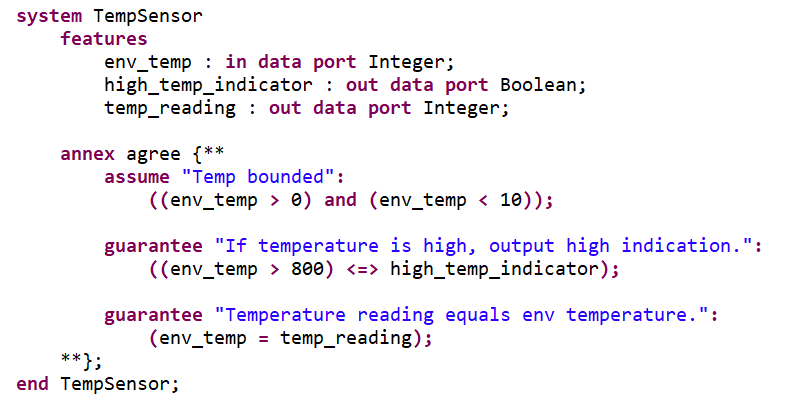
\includegraphics[width=1.0\textwidth]{images/agreeContract2.png}
	\caption{The AGREE Contract for an AADL Component Type}
	\label{fig:agreeContract}
	%\vspace{-0.2in}
	%\vspace{-0.1in}
	\end{center}
\end{figure}

An example of an AGREE contract is shown in Figure~\ref{fig:agreeContract} and is placed in the context of the AADL temperature sensor component shown in Figure~\ref{fig:aadlComponent}.  An AGREE contract consists of {\em assumptions} on the inputs of AADL components that constrain what the component sees from the environment and {\em guarantees} on the outputs that constrain how the component behaves given its environment. In this example, the assumption restricts the environmental temperature to be within a range of values; the guarantee defines the behavior of the component given the environment. 

Since our desire was to facilitate {\em behavioral error propagation}, AGREE was a suitable and obvious choice for the nominal verification tooling. 

Through AGREE, the nominal model is translated into the dataflow programming language Lustre~\cite{Halbwachs91:IEEE} that is used as input to the JKind model checker~\cite{2017arXiv171201222G}. JKind uses a series of backend SMT-solvers to generate proofs of the top level AGREE properties specified in the model. When there exists a trace such that a property is invalid, JKind provides a {\em counterexample} showing the system trace in which the property is violated. An example of this is shown in Figure~\ref{fig:coex}. 

\begin{figure}[h!]
	%\vspace{-0.1in}
	\begin{center}
	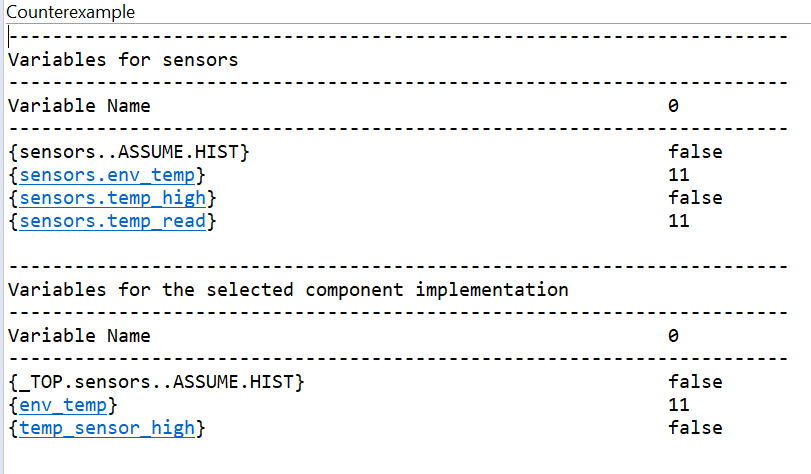
\includegraphics[width=1.0\textwidth]{images/coex.png}
	\caption{A Counterexample to an Invalid Property}
	\label{fig:coex}
	%\vspace{-0.2in}
	%\vspace{-0.1in}
	\end{center}
\end{figure}

The model checker takes an adversarial role in the proof process by trying to find paths such that the proof is violated. If none exist, then the results are valid. This adversarial role is exactly what we wished to harness for this kind of analysis. If we allow faults to be active, but leave them unconstrained, this allows the model checker to determine if certain faults could lead to a violation of a property. These counterexamples could then contain fault information. 

Given that AGREE guarantees define the {\em output} behavior of components, any connected component's assumptions rely on those guarantees. If an assumption is violated, the guarantee may not hold. By associating a fault with the output of a component, this fault -- when active -- may violate assumptions and guarantees along the signal flow within a system. This was our goal; we wished to view the behavioral propagation of an active fault. 

\subsection{Implementation Architecture}
\label{sec:implArchitecture}
The safety annex is written in Java as a plug-in for the OSATE AADL toolset, which is built on Eclipse.  It is not designed as a stand-alone extension of the language, but works with behavioral contracts specified using the AGREE annex for AADL~\cite{NFM2012:CoGaMiWhLaLu}. 
The architecture of the Safety Annex is shown in Figure~\ref{fig:plugin-arch}.

\begin{figure}[h]
	\begin{center}
		%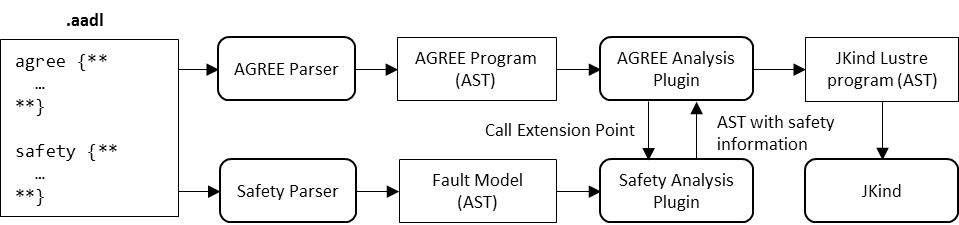
\includegraphics[trim=0 400 430 0,clip,width=0.85\textwidth]{images/arch.png}
		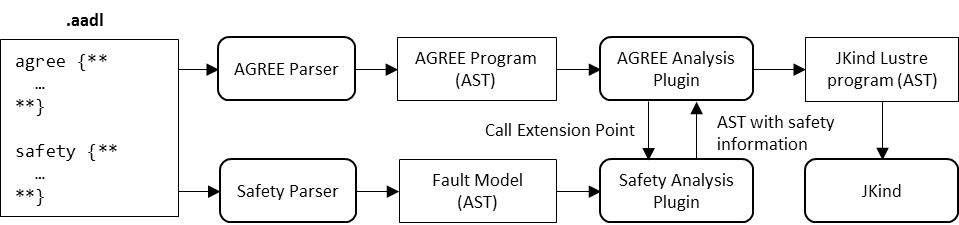
\includegraphics[width=\textwidth]{images/arch.png}
	\end{center}
	%\vspace{-0.2in}
	\caption{Safety Annex Plug-in Architecture}
	\label{fig:plugin-arch}
	%\vspace{-0.2in}
\end{figure}

The safety language extension resides in an annex of AADL and the faults defined therein are translated into an abstract syntax tree and inserted into the AGREE program. The AGREE program contains the building blocks for the translation into Lustre which is the program directly analyzed by JKind.  

When performing fault analysis, the fault definitions defined in the safety annex extend the AGREE contracts to allow faults to modify the behavior of component outputs. The temperature sensor subcomponent shown in Figure~\ref{fig:agreeContract} encoded into Lustre is shown in Figure~\ref{fig:lustreTempNode}\footnote{The Lustre code is slightly simplified for readability.}.

\begin{figure}[h]
	\begin{center}
		%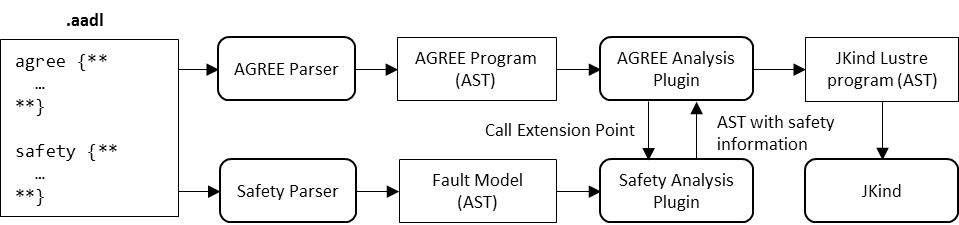
\includegraphics[trim=0 400 430 0,clip,width=0.85\textwidth]{images/arch.png}
		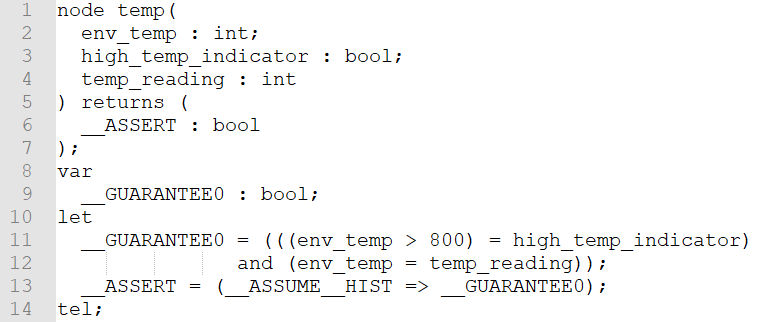
\includegraphics[width=0.8\textwidth]{images/lustreTempNode.png}
	\end{center}
	%\vspace{-0.2in}
	\caption{Temperature Component in Lustre}
	\label{fig:lustreTempNode}
	%\vspace{-0.2in}
\end{figure}

The inputs and outputs (lines 2-4) correspond directly to the AADL inputs and outputs of the component; likewise, the guarantee (\texttt{\_\_GUARANTEE0}) corresponds to the guarantee on the outputs. The \texttt{\_\_ASSERT} statement on line 13 states that as long as the assumptions hold, the guarantee is implied. 

From the perspective of fault analysis, we want to insert a fault on the output of the component. This fault may or may not be active -- it is up to the model checker. To this end, we specify three variables per potentially faulty output: \texttt{fault\_nominal}, \texttt{fault\_trigger}, and \texttt{fail\_val}. If the trigger is true, then output failure value, else output nominal value. This can be seen in Figure~\ref{fig:lustreTempNodeFault}: the new variables are assigned as inputs (lines 4-6) and the assert statement in line 20 shows the triggering behavior.

\begin{figure}[h]
	\begin{center}
		%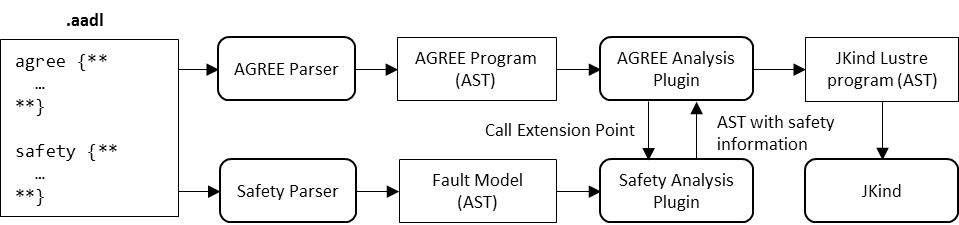
\includegraphics[trim=0 400 430 0,clip,width=0.85\textwidth]{images/arch.png}
		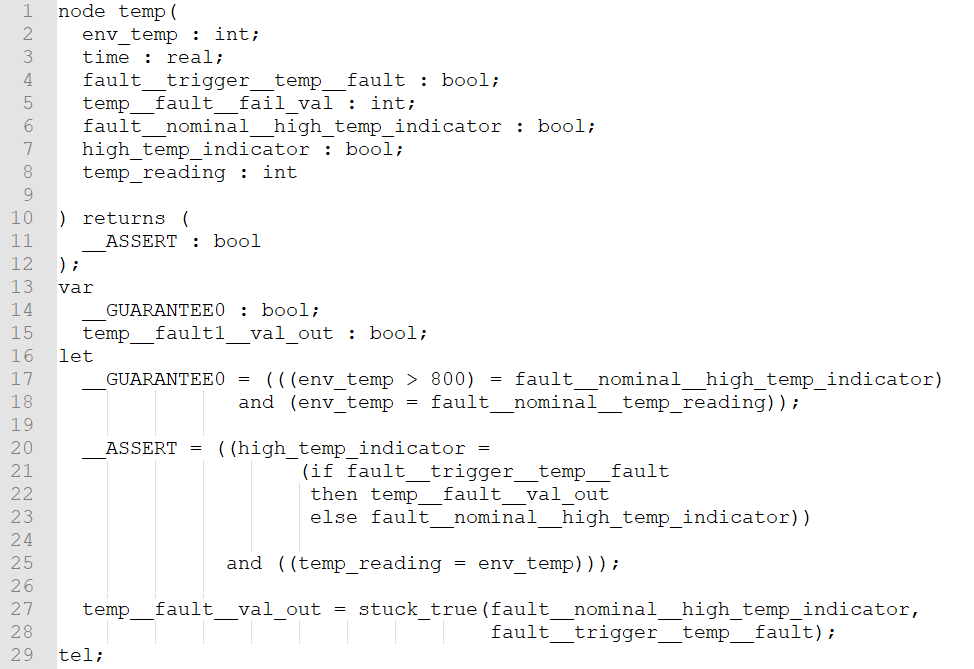
\includegraphics[width=0.8\textwidth]{images/lustreTempNodeFault.png}
	\end{center}
	%\vspace{-0.2in}
	\caption{Temperature Component with Fault in Lustre}
	\label{fig:lustreTempNodeFault}
	%\vspace{-0.2in}
\end{figure}

This allows for the possibility of active faults, but when the faults are inactive, the nominal value is simply passed through. Line 27 of Figure~\ref{fig:lustreTempNodeFault} shows a call to what we call a {\em fault node}; this is the code that specifies the behavior of an active fault. The fault node \texttt{stuck\_true} is shown in Figure~\ref{fig:lustreFaultNode}. The behavior of an active fault is to output {\em true}. The \texttt{trigger} input to the fault node corresponds directly with the trigger defined in the temperature node of Figure~\ref{fig:lustreTempNodeFault} on line 4. 

\begin{figure}[h]
	\begin{center}
		%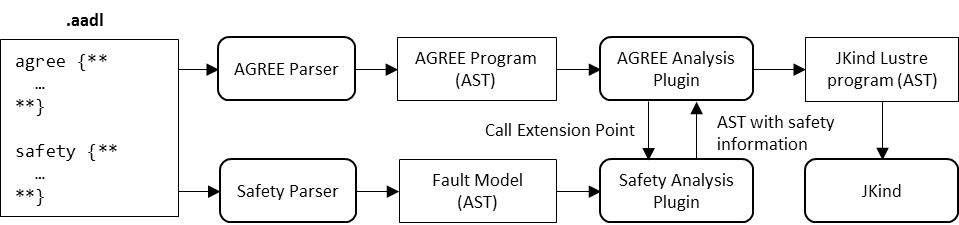
\includegraphics[trim=0 400 430 0,clip,width=0.85\textwidth]{images/arch.png}
		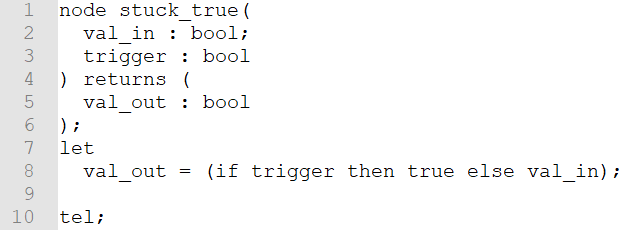
\includegraphics[width=0.8\textwidth]{images/lustreFaultNode.png}
	\end{center}
	%\vspace{-0.2in}
	\caption{A Fault Node in Lustre}
	\label{fig:lustreFaultNode}
	%\vspace{-0.2in}
\end{figure}
 
The model elements are translated into Lustre formulae. These are represented in JKind as a transition system, and reasoning is performed using $k$-induction. At each time-step of analysis, every formula in the model is given an assignment based on the constraints over that formula. If every assignment results in a provable property over $k$ steps of induction, the property holds. When performing safety analysis over the model, each fault is defined as an {\em activation literal} and is unconstrained. If the assignment to an activation literal is {\em true}, this corresponds to an active fault and potentially violated guarantee. If that assignment violates a guarantee, then this violation will be reflected in the analysis results. At a system level, it can be seen if a violated guarantee will in turn violate the top level property. Hence it is seen how active faults at leaf level components violate the system level properties. 

This analysis approach allows for implicit propagation of violations throughout the system. It also allows for arbitrary temporal activations of faults. There are no explicit constraints put on faults stating when an activation can occur, which allows the model checking procedure free reign to activate the faults at the worst possible times. If there are dependencies regarding fault activations, these are handled through the use of explicit error propagations (see Section~\ref{sec:propogation}).

The main constraint put on the model checker in terms of the activation of faults consist of {\em fault hypothesis statements}. These constrain the model by stating either the number of faults that may be active at once, or the overall probability threshold that is allowed. In the latter case, each fault has an associated probability; assuming independence, the probability of a set of faults occurring should not be less than the threshold defined. 

There are two different types of fault analysis that can be performed on a fault model: verification in the presence of faults or the generation of minimal cut sets. The Safety Annex plugin intercepts the AGREE program and adds fault model information depending on which type of fault analysis is being run. For more information on types of fault analysis, see Section~\ref{sec:analysisResults}.










	\chapter{Compositional Minimal Cut Set Generation}
\label{chap:mcsGen}

Given the importance of minimal cut set computations for industrial sized systems, much research has been done on their generation (e.g.,~\cite{fta:survey,rauzy1993new,historyFTA,Bozzano:2010:DSA:1951720,rausand2003system}). As described in preliminary sections, the methods of cut set generation have varied greatly depending on how the system is modeled -- transition systems, state machines, decision diagrams, to name a few-- and what kind of model checking is performed -- symbolic algorithms, bounded model checking, etc. Compositional minimal cut set generation has not, to our knowledge, been previously explored. Due to the compositional nature of the verification it is difficult to see how faults that are {\em not} present in the current layer will affect the component behaviors and proofs of the current layer. This information needs to get passed through the layers of the model somehow. 

A contribution of this dissertation is providing a means for the compositional generation of minimal cut sets. In order to perform this kind of computation compositionally, a pre-existing framework was required. \danielle{Instead of having full paragraphs here for each piece, should I refer to the sections where these things are defined fully? Or provide a short preview here to eliminate the need to jump around in the document? Or both?}

(1) A rich modeling language was needed that allowed for the hierarchical definition of the model. The Architecture Analysis and Design Language (AADL)~\cite{aerospace2012sae} was chosen; AADL is an SAE International standard language that provides a unifying framework for describing the system architecture for performance-critical, embedded, real-time systems~\cite{AADL_Standard,FeilerModelBasedEngineering2012}. %Furthermore, AADL supports language extensions called {\em annexes} and there are open-source verification options that reason over AADL models.

(2) A compositional verification framework was required for the analysis of AADL models. The Assume-Guarantee Reasoning Environment (AGREE) is a tool for formal analysis of behaviors in AADL models~\cite{NFM2012:CoGaMiWhLaLu}.  It is implemented as an AADL annex and annotates AADL components with formal behavioral contracts. Each component's contracts can include assumptions and guarantees about the component's inputs and outputs respectively, as well as predicates describing how the state of the component evolves over time. AGREE translates an AADL model and the behavioral contracts into the dataflow programming language Lustre~\cite{Halbwachs91:IEEE} and then queries the model checker JKind~\cite{2017arXiv171201222G} to conduct the back-end analysis. The analysis can be performed compositionally or monolithically.

(3) A safety specific language was required that allows for the definitions of faults over component outputs and the model checker provides safety specific information and proofs about the fault model. In the early stages of this research, the Safety Annex for AADL was developed. The Safety Annex for AADL and its supporting extensions to the AADL tools provide the ability to reason about faults and faulty component behaviors in AADL models~\cite{Stewart17:IMBSA,stewart2020safety, nasaFinalReport}. In the Safety Annex approach, AGREE contracts are used to define the nominal behavior of system component and the nominal model is verified using JKind. The Safety Annex implementation weaves faults into the nominal model and analyzes the behavior of the system in the presence of faults. The tool supports behavioral specification of faults and their implicit propagation through behavioral relationships in the model and provides support to capture binding relationships between hardware and software components of the system. %For more information on the Safety Annex, see Chapter~\ref{chap:faultModeling}.

The remainder of this chapter describes compositional minimal cut set generation. First, the formal background and definitions required to understand the approach are supplied, then the proofs and algorithms are given. The implementation of these algorithms in the Safety Annex are then described.

\section{The High Level Idea and Approach}
Recently, Ghassabani et al. developed an algorithm that traces a safety property to a minimal set of model elements necessary for proof; this is called the \textit{all minimal inductive validity core} algorithm (\aivcalg)~\cite{GhassabaniGW16,Ghassabani2017EfficientGO,bendik2018online}. Inductive validity cores produce the minimal set of model elements necessary to prove a property. Each set contains the \emph{behavioral contracts} -- the requirement specifications for components -- of the model used in a proof. When the \aivcalg algorithm is run, this gives the minimal set of contracts required for proof of a safety property. If all of these sets are obtained, we have insight into every proof path for the property. Thus, if we violate at least one contract from every MIVC set, we have in essence ``broken" every proof path. This is the information that is used to perform fault analysis using MIVCs.

Safety analysts are often concerned with faults in the system, i.e., when components or subsystems deviate from nominal behavior, and the propagation of errors through the system. To this end, the model elements included in the reasoning process of the \aivcalg algorithm are not only the contracts of the system, but faults as well. This will provide additional insight into how an active fault may violate contracts that directly support the proof of a safety property. 

Before the specifics of the algorithm and proofs can be discussed, some background definitions are required. Throughout this chapter, a running example is referenced and we provide the description here.

\section{Running Example}
\label{sec:example}

To illustrate the generation of minimal cut sets through the use of IVCs, we present a running example of a sensor system in a Pressurized Water Reactor (PWR). In a typical PWR, the core inside of the reactor vessel produces heat. Pressurized water in the primary coolant loop carries the heat to the steam generator. Within the steam generator, heat from the primary coolant loop vaporizes the water in a secondary loop, producing steam. The steamline directs the steam to the main turbine, causing it to turn the turbine generator, which produces electricity. There are a few important factors that must be considered during safety assessment and system design. An unsafe climb in temperature can cause high pressure and hence pipe rupture, and high levels of radiation could indicate a leak of primary coolant. The following sensor system can be thought of as a subsystem within a PWR that monitors these factors. A diagram of the AADL model is shown in Figure~\ref{fig:sensorSys} and represents a highly simplified version of a safety critical system. \danielle{May add cartoon figure demonstrating this model/process later - depending on space. Also can adjust figure placement after rewriting, adding, and cutting is done.}

\begin{figure*}[h!]
	%\vspace{-2em}
	\begin{center}
		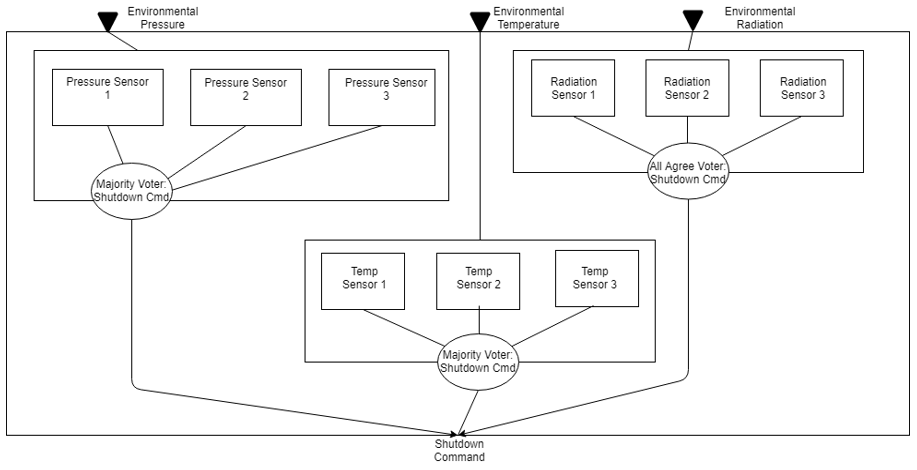
\includegraphics[width=0.6\textwidth]{images/sensorSys.PNG}
	\end{center}
	\vspace{-1em}
	\caption{Pressurized Water Reactor Sensor System}
	\label{fig:sensorSys}
	%\vspace{-2em}
\end{figure*}

\subsection{PWR Nominal Model}
The ``top-level" system is an abstraction of the PWR and contains sensor subsystems. The subsystems contain sensors that monitor pressure, temperature, and radiation. Environmental inputs are fed into each sensor in the model and the redundant sensors monitor temperature, pressure, or radiation respectively. If temperature, pressure, or radiation is too high, a shut down command is sent from the sensors to the parent components. 

The temperature, pressure, and radiation sensor subsystems use a voting mechanism on the redundant sensor values and will send a shut down command based on this output. The safety property of interest in this system is: \emph{shut down when and only when we should}; the AGREE guarantee stating this property is shown in Figure~\ref{fig:shutdownGuar}. 

\begin{figure*}[h!]
	%\vspace{-2em}
	\begin{center}
		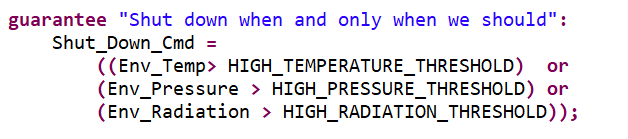
\includegraphics[width=0.5\textwidth]{images/sensorGuar.PNG}
	\end{center}
	\vspace{-2em}
	\caption{Sensor System Safety Property}
	\label{fig:shutdownGuar}
	%\vspace{-2em}
\end{figure*}

The safety of the system requires a shut down to take place if the temperature, pressure, or radiation levels become unsafe; thus, a threshold is introduced and if any sensor subsystem reports passing that threshold, a shutdown command is sent. But on the other hand, we do not want to shut down the system if it is not necessary. If a sensor reports high temperature erroneously and a shut down occurs, this costs time and money. 

Supporting guarantees are located in each sensor subsystem and correspond to temperature, pressure, and radiation sending a shut down command if sensed inputs are above a given threshold. Each sensor has a similar guarantee. 

\subsection{PWR Fault Model}
The faults that are of interest in this example system are any one of the sensors failing high or low. If sensors report high and a shut down command is sent, we shut down when we should not. On the other hand, if sensors report low when it should be high, a shut down command is not sent and we do not shut down when we should. For the remainder of this example, we focus on the failures when sensors report low when they should not.

Two faults are defined with the safety annex for each sensor in the system. An example of a temperature sensor fault stuck at high is shown in Figure~\ref{fig:tempSensorFault}.

\begin{figure*}[h!]
	\vspace{-2em}
	\begin{center}
		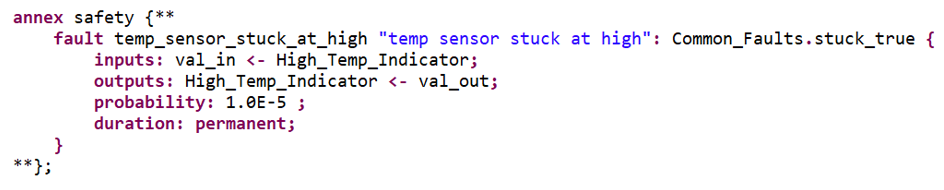
\includegraphics[width=0.8\textwidth]{images/tempSensorFault.PNG}
	\end{center}
	\vspace{-2em}
	\caption{Fault on Temperature Sensor Defined in the Safety Annex for AADL}
	\label{fig:tempSensorFault}
	\vspace{-2em}
\end{figure*}

The Safety Annex provides a way to weave the faults into the nominal model by use of the \emph{inputs} and \emph{outputs} keywords. This allows users to define a fault and attach it to the output of a component. If the fault is active, the error can then in essence violate the guarantees of this component and possibly the assumptions of downstream components~\cite{stewart2020safety}. The activation of a fault is not up to the user, but instead left up to the backend model checker, JKind, to determine if the activation of this fault will contribute to a violation of higher level guarantees. If so, it can be activated during the analysis.

For simplicity, throughout this paper we refer only to faults that fail low (i.e., the environmental input is actually high which warrants a shut down command, but the sensor reports that it is within safe ranges). This simplification is presented to keep the example and results described concise. For ease of reference, a table is provided giving model elements of interest in the sensor example. We refer to these throughout this section. Note: the thresholds vary for pressure, temperature, and radiation. These are given as constants $T_p$, $T_t$, and $T_r$ respectively. The shutdown command is defined notationally as $S$.  The faults are shown as ``fail low" which correspond to the temp (or pressure or radiation) being high, but the sensor reports safe ranges. We also do not list all guarantees and assumptions that are in the model, but only the ones of interest for this analysis. \danielle{Still messing around with how to display this in a way that it isn't messy, doesn't take up a ton of space, and am not currently happy with this approach. But I really hated the tables. Too much info for what is actually needed. Will keep working on this.}

\begin{description}[parsep=0.3ex]
 \item[PWR System:] $P = ((temp$ $>$ $T_t)$ $\lor$ $ (pressure$ $>$ $ T_p)$  $\lor$ $ (radiation$ $>$ $ T_r)) \iff S$\\
 \item[Temp Subsystem]: $G_t = temp$ $>$ $ T_t \iff S$\\
 \item[Pressure Subsystem:] $G_p = pressure$ $>$ $ T_p \iff S$\\
 \item[Radiation Subsystem:] $G_r = radiation$ $>$ $ T_r \iff S$\\
 \item[Temp Sensors (3):] $g_p = pressure$ $>$ $ T_p \iff S$, Fault $f_{ti}$: fails low for $i = 1, 2, 3$.\\
\item[Pressure Sensors (3):] $g_r = radiation$ $>$ $ T_r \iff S$, Fault $f_{pi}$: fails low for $i = 1, 2, 3$. \\
 \item[Radiation Sensors (3):] $g_r = radiation$ $>$ $ T_r \iff S$, Fault $f_{ri}$: fails low for $i = 1, 2, 3$\\
 \end{description}


\begin{comment}
\begin{center}
\resizebox{0.5\textwidth}{!}{%
    \begin{tabular}{ | c | c | c |}
      \hline
      \thead{Component} & \thead{Layer of Analysis} & \thead{Guarantee}\\
      \hline
      ReactorSys & Top &  \makecell{Safety Property $P$: \\ $((temp$ $>$ $T_t)$ $\lor$ $ (pressure$ $>$ $ T_p)$  $\lor$ $ (radiation$ $>$ $ T_r))$ \\ $\iff SHUTDOWN$}    \\
      \hline
      TempSys & Leaf  &  \makecell{Guarantee $G_t$: \\  $temp$ $>$ $ T_t \iff SHUTDOWN$}   \\
      \hline
      PressureSys & Leaf  &  \makecell{Guarantee $G_p$: \\ $pressure$ $>$ $ T_p \iff SHUTDOWN$}    \\
	\hline
      RadiationSys & Leaf  &  \makecell{Guarantee $G_r$: \\ $radiation$ $>$ $ T_r \iff SHUTDOWN$}   \\
      \hline
    \end{tabular}}
  \end{center}

\begin{center}
\resizebox{0.5\textwidth}{!}{%
    \begin{tabular}{ | c | c | c |}
      \hline
      \thead{Component} & \thead{Layer of Architecture} & \thead{Faults}\\
      \hline
      Temp Sensors (3) & \makecell{Leaf \\ Components} & \makecell{$f_{t}$: fail low}  \\
      \hline
	Pressure Sensors (3) & \makecell{Leaf \\ Components} & \makecell{$f_{p}$: fail low}  \\
      \hline
	Radiation Sensors (3) & \makecell{Leaf \\ Components} & \makecell{$f_{r}$: fail low}  \\
      \hline
    \end{tabular}}
  \end{center}



\subsection{Using this Example in the Generation of Minimal Cut Sets}
Step by step, we outline how minimal cut sets are generated through the \aivcalg algorithm using the sensor system as an example. For ease of reference, a table is provided giving model elements of interest in the sensor example. We refer to these throughout this section. Note: the thresholds vary for pressure, temperature, and radiation. These are given as constants $T_p$, $T_t$, and $T_r$ respectively. We also do not list all guarantees and assumptions that are in the model, but only the ones of interest for this analysis.

\begin{center}
\resizebox{\textwidth}{!}{%
    \begin{tabular}{ | c | c | c |}
      \hline
      \thead{Component} & \thead{Layer of Analysis} & \thead{Guarantee}\\
      \hline
      ReactorSys & Top &  \makecell{Safety Property $P$: \\ $((temp$ $>$ $T_t)$ $\lor$ $ (pressure$ $>$ $ T_p)$  $\lor$ $ (radiation$ $>$ $ T_r))$ \\ $\iff SHUTDOWN$}    \\
      \hline
      TempSys & Leaf  &  \makecell{Guarantee $g_t$: \\  $temp$ $>$ $ T_t \iff SHUTDOWN$}   \\
      \hline
      PressureSys & Leaf  &  \makecell{Guarantee $g_p$: \\ $pressure$ $>$ $ T_p \iff SHUTDOWN$}    \\
	\hline
      RadiationSys & Leaf  &  \makecell{Guarantee $g_r$: \\ $radiation$ $>$ $ T_r \iff SHUTDOWN$}   \\
      \hline
    \end{tabular}}
  \end{center}

\begin{center}
%\resizebox{\textwidth}{!}{%
    \begin{tabular}{ | c | c | c |}
      \hline
      \thead{Component} & \thead{Layer of Architecture} & \thead{Faults}\\
      \hline
      Temp Sensors (3) & \makecell{Leaf \\ Components} & \makecell{$f_{t}$: fail low}  \\
      \hline
	Pressure Sensors (3) & \makecell{Leaf \\ Components} & \makecell{$f_{p}$: fail low}  \\
      \hline
	Radiation Sensors (3) & \makecell{Leaf \\ Components} & \makecell{$f_{r}$: fail low}  \\
      \hline
    \end{tabular}
  \end{center}

The first two steps of this process are performed top down in conjunction with JKind analysis over a program. Thus, the top layer is analyzed first, then the next and so on. Steps 3 and 4 proceed after all MIVCs for each layer have been generated. We walk through this sensor system example in this fashion. 

\textbf{Step 1a: Preprocessing top layer.} The preprocessing step inserts specific MIVC elements into the Lustre program. The MIVC elements are the model elements considered in the constraint system for a given property. The Safety Annex provides the means to define a fault over the output of a component. This fault is given an unassigned \emph{trigger} Boolean literal in Lustre. If the trigger literal is true, the output of the component is changed. If not, the output remains equivalent to the nominal output of this component~\cite{stewart2020safety, Stewart17:IMBSA}. This trigger in Lustre is called a \emph{fault activation literal}. The IVC elements required in order to perform this transformation are these fault activation literals as well as guarantees. The basic rules used to insert these additional literals into Lustre depend on the analysis layer of that is being formed in Lustre and are as follows. 
\begin{itemize}
\item Leaf layer of analysis: only fault activation literals are added.
\item Middle or top layers: guarantees are added and if a direct subcomponent is a leaf component of the architecture and faults are defined on its outputs, then these faults are also added.
\end{itemize}

At the top level, guarantees of the sensor subsystems are the IVC elements.
$$\boxed{g_t, g_p, g_r}$$

There are distinct constraint systems, one for each property being proved. In this system at the top layer, there is a single property $P$; this results in the following constraint system. 
$$\boxed{C = \{g_t, g_p, g_r, \neg P\}}$$

\textbf{Step 2a: Generate all MIVCs for the constraint system at the top layer.} In order to prove $P$, all three guarantees from the sensor subsystem level are required. 
$$\boxed{MIVC(P) = \{g_t, g_p, g_r\}}$$. 

\textbf{Step 1b: Preprocessing leaf layer.} Model elements for the IVC algorithm consideration are the faults for each sensor, for instance temperature sensors:
$$\boxed{f_{t1}, f_{t2}, f_{t3}}$$ 

The resulting constraint system for the temperature sensor subsystem layer is:
$$\boxed{C = \{\neg f_{t1}, \neg f_{t2}, \neg f_{t3}, \neg g_t\}}$$

\textbf{Step 2b: Generate all MIVCs for the constraint system at the leaf layer.} Due to the majority voting mechanism, the MIVCs show all possible pairs of faults restricted to \emph{false}. This means, if any combination of two faults do not occur, then the guarantees at the temperature sensor subsystem level are satisfied. 
$$\boxed{
	\begin{aligned}
		MIVC_1(g_t) = \{\neg f_{t1}, \neg f_{t2}\} \\
		MIVC_2(g_t) = \{\neg f_{t1}, \neg f_{t3}\} \\
		MIVC_3(g_t) = \{\neg f_{t2}, \neg f_{t3}\}
	\end{aligned}
}$$

At this point, all MIVCs have been successfully generated (which is a requirement of the following algorithms) and we can move on to the generation of minimal cut sets. 

\textbf{Step 3a: Generate MCSs using a hitting set algorithm at the top layer.} Our single MIVC in this case will reveal three associated MCSs. (Notice: $MCS_1 \cap MIVC(P) \neq \emptyset$, and same for $MCS_2$ and $MCS_3$, thus these are hitting sets.)
 $$\boxed{
	\begin{aligned}
		MCS_1(top) = \{g_t\} \\
		MCS_2(top) = \{g_p\} \\
		MCS_3(top) = \{g_r\}
	\end{aligned}
}$$

\textbf{Step 4a: Transform MCSs into MinCutSets at the top layer.} Given that only guarantees are found in the MCSs at this layer, recursion is used to find the faults that cause violation of these guarantees. Using this recursion on $MCS_1$, we show the process further. 

\textbf{Step 3b: Generate MCSs using a hitting set algorithm at the leaf layer.} In step 2b, we found all MIVCs for the contract $g_t$ and send these to the hitting set algorithm. The resulting MCSs are: 
 $$\boxed{
	\begin{aligned}
		MCS_1(leaf) = \{\neg f_{t1}, \neg f_{t2}\} \\
		MCS_2(leaf) = \{\neg f_{t1}, \neg f_{t3}\} \\
		MCS_3(leaf) = \{\neg f_{t2}, \neg f_{t3}\}
	\end{aligned}
}$$

Only constrained faults are found in these MCSs, so we simply remove those constraints and have found the MinCutSets for the contracts $g_t$. These are returned and replace this contract in the top layer $MCS_1(top)$. Here is the end result for $MCS_1(top)$; this can be understood as three of the total minimal cut sets for $P$. 

\begin{equation*}
MCS_1(top) \rightarrow \left\{ \,
\begin{IEEEeqnarraybox}[][c]{l?s}
\IEEEstrut
MinCutSet_1(P) = \{f_{t1}, f_{t2}\}, \\
MinCutSet_2(P) = \{f_{t1},  f_{t3}\}, \\
MinCutSet_3(P) = \{f_{t2}, f_{t3}\}
\IEEEstrut
\end{IEEEeqnarraybox}
\right.
\end{equation*}

After all replacements have been made, we are left with all minimal cut sets for the property of interest ($P$ in this example). 

\end{comment}











\section{Preliminaries for Minimal Cut Set Generation}
\label{sec:prelimMCS}
In this research we consider \emph{safety properties} over infinite-state machines. The states are vectors of variables that define the values of state variables. We assume there are a set of legal \emph{initial states} and the safety property is specified as a formula over state variables. A \emph{reachable state space} means that all states are reachable from the initial state. 

Given a state space $U$, a transition system $(I,T)$ consists of an
initial state predicate $I : U \to \bool$ and a transition step
predicate $T : U \times U \to \bool$.
We define the notion of
reachability for $(I, T)$ as the smallest predicate $\reach : U \to
\bool$ which satisfies the following formulas:
\begin{gather*}
  \forall u.~ I(u) \Rightarrow \reach(u) \\
  \forall u, u'.~ \reach(u) \land T(u, u') \Rightarrow \reach(u')
\end{gather*}
A safety property $P : U \to \bool$ is a state predicate. A safety
property $P$ holds on a transition system $(I, T)$ if it holds on all
reachable states, i.e., $\forall u.~ \reach(u) \Rightarrow P(u)$,
written as $\reach \Rightarrow P$ for short. When this is the case, we
write $(I, T)\vdash P$.

\subsection{Induction}
For an arbitrary transition system $(I, T)$, computing reachability
can be very expensive or even impossible. Thus, we need a more
effective way of checking if a safety property $P$ is satisfied by the
system. The key idea is to over-approximate reachability. If we can
find an over-approximation that implies the property, then the
property must hold. Otherwise, the approximation needs to be refined.

A good first approximation for reachability is the property itself.
That is, we can check if the following formulas hold:
\begin{gather}
  \forall s.~ I(s) \Rightarrow P(s)
  \label{eq:1-ind-base} \\
  \forall s, s'.~ P(s) \land T(s, s') \Rightarrow P(s')
  \label{eq:1-ind-step}
\end{gather}
If both formulas hold then $P$ is {\em inductive} and holds over the
system. If (\ref{eq:1-ind-base}) fails to hold, then $P$ is violated
by an initial state of the system. If (\ref{eq:1-ind-step}) fails to
hold, then $P$ is too much of an over-approximation and needs to be
refined.

The JKind model checker used in this research uses {\em
  $k$-induction} which unrolls the property over $k$ steps of the
transition system. For example, 1-induction consists of formulas
(\ref{eq:1-ind-base}) and (\ref{eq:1-ind-step}) above, whereas
2-induction consists of the following formulas:
\begin{gather*}
\forall s.~ I(s) \Rightarrow P(s) \\
\forall s, s'.~ I(s) \land T(s, s') \Rightarrow P(s') \\
\forall s, s', s''.~ P(s) \land T(s, s') \land P(s') \land T(s',
  s'') \Rightarrow P(s'')
\end{gather*}
That is, there are two base step checks and one inductive step check.
In general, for an arbitrary $k$, $k$-induction consists of $k$
base step checks and one inductive step check as shown in
Figure~\ref{fig:k-induction} (the universal quantifiers on $s_i$ have
been elided for space). We say that a property is $k$-inductive if it
satisfies the $k$-induction constraints for the given value of $k$.
The hope is that the additional formulas in the antecedent of the
inductive step make it provable.

\begin{figure}
\begin{gather*}
I(s_0) \Rightarrow P(s_0) \\[-2pt]
%
\vdots \\[2pt]
%
I(s_0) \land T(s_0, s_1) \land \cdots \land T(s_{k-2}, s_{k-1})
\Rightarrow P(s_{k-1}) \\[2pt]
%
P(s_0) \land T(s_0, s_1) \land \cdots \land P(s_{k-1}) \land
T(s_{k-1}, s_k) \Rightarrow P(s_k)
\end{gather*}
\caption{$k$-induction formulas: $k$ base cases and one inductive
  step}
\label{fig:k-induction}
\end{figure}

In practice, inductive model checkers often use a combination of the
above techniques. Thus, a typical conclusion is of the form ``$P$ with
lemmas $L_1, \ldots, L_n$ is $k$-inductive''.

\subsection{The SAT Problem}
Boolean Satisfiability (SAT) solvers attempt to determine if there exists a total truth assignment to a given propositional formula, that evaluates to TRUE. Generally, a propositional formula is any combination of the disjunction and conjunction of literals (as an example, $a$ and $\neg a$ are literals). For a given unsatisfiable problem, solvers try to generate a proof of unsatisfiability; this is generally more useful than a proof of satisfiability. Such a proof is dependent on identifying a subset of clauses that make the problem unsatisfiable (UNSAT). 

SAT solvers in model checking work over a constraint system to determine satisfiability. A \textit{constraint system} $C$ is an ordered set of $n$ abstract constraints $\{C_1, C_2, ..., C_n\}$ over a set of variables. The constraint $C_i$ restricts the allowed assignments of these variables in some way~\cite{liffiton2016fast}. Given a constraint system, we require some method of determining, for any subset $S \subseteq C$, whether $S$ is \textit{satisfiable} (SAT) or \textit{unsatisfiable} (UNSAT). When a subset $S$ is SAT, this means that there exists an assignment allowed by all $C_i \in S$; when no such assignment exists, $S$ is considered UNSAT. 

There are several ways of translating a propositional formula into clauses such that satisfiability is preserved~\cite{een2003temporal}. By performing this translation, $k$-inductive model checkers are able to utilize parallel SAT-solving engines to glean information about the proof of a safety property at each inductive step. Expression of the base and induction steps of a temporal induction proof as SAT problems is straightforward. As an example, we look at an arbitrary base case from Figure~\ref{fig:k-induction}.

\begin{gather*}
I(s_0) \land T(s_0, s_1) \land \cdots \land T(s_{k-2}, s_{k-1})
\land \neg P(s_{k-1})
\end{gather*}

When proving correctness it is shown that the formulas are \emph{unsatisfiable}. If an $n^{th}$ inductive-step is unsatisfiable, that means following an $n$-step trace where the property holds, there exists no next state where it fails, i.e., the property $P$ is provable.





\section{Formalization of the Method}
\label{sec:formMCS}
\danielle{Section desperately needs figures of some kind to break up the text. Will try to make a few small ones of PWR example results.}
Compositional analysis proceeds from the top layer of the architecture down through the system model; faults are defined on leaf level components and guarantees are defined on all components. Due to the difference in analysis per layer, this section focuses on the formalism per layer type we are in. 

Given an initial state $I$ and a transition relation $T$ consisting of conjunctive constraints as defined in section~\ref{sec:prelim}. The nominal guarantees of the system, $G$, consist of conjunctive constraints $g \in G$. Given no faults, each $g$ is one of the transition constraints $T_i$ where:

\begin{gather}
T_n = g_1 \land  g_2 \land \cdots \land g_n
\label{eq:Tn}
\end{gather}

We assume the property holds of the nominal relation $(I,T_n) \vdash P$. Given that our focus is on safety analysis in the presence of faults, let the set of all faults in the system be  denoted as $F$. A fault $f \in F$ is a deviation from the normal constraint imposed by a guarantee. Any ``faults" in a mid-layer are simply violated guarantees, or deviations from normal behavior.

\subsection{Top Layer of Compositional Analysis}
Since faults are defined at leaf layers of the architecture, the top (and middle) layers only contain guarantees in the analysis. The \aivcalg algorithm collects all {\em minimal unsatisfiable subsets} (MUSs) of a given transition system in terms of the \textit{negation} of the top level property~\cite{Ghassabani2017EfficientGO,bendik2018online}. Formally, an MUS of a constraint system $C$ is a set $M \subseteq C$ such that $M$ is unsatisfiable and $\forall c \in M$ : $M \setminus \{c\}$ is satisfiable. The MUSs are the minimal explanation of the infeasibility of this constraint system; equivalently, these are the minimal sets of model elements necessary for proof of the safety property.

Returning to our running example, this can be illustrated by the following. Given the constraint system $C = \{G_p, G_t, G_r, \neg P\}$, a minimal explanation of the infeasability of this system is the set $\{G_p, G_t, G_r,\}$. If all three guarantees hold, then $P$ is provable. 

A related set is a {\em minimal correction set} (MCS); a MCS $M$ of a constraint system $C$ is a subset $M\subseteq C$ such that $C \setminus M$ is satisfiable and $\forall S \subset M$ : $C \setminus S$ is unsatisfiable. A MCS can be seen to ``correct'' the infeasability of the constraint system by the removal from $C$ the constraints found in an MCS.

In the case of an UNSAT system, we may ask: what will correct this unsatisfiability? Returning to the PWR example, we can find the MCSs of the top level constraint system: $MCS_1 = \{G_t\}$, $MCS_2 = \{G_p\}$, $MCS_3 = \{G_r\}$. If any single guarantee is violated, a shut down from that subsystem will not get sent when it should and the safety property $P$ will be violated. 

A duality exists between the MUSs of a constraint system and the MCSs as established by Reiter \cite{reiter1987theory}. This duality is defined in terms of \textit{Minimal Hitting Sets} (\textit{MHS}). A hitting set of a collection of sets $A$ is a set $H$ such that every set in $A$ is ``hit'' by $H$; $H$ contains at least one element from every set in $A$. Every MUS of a constraint system is a minimal hitting set of the system's MCSs, and likewise every MCS is a minimal hitting set of the system's MUSs~\cite{liffiton2016fast, reiter1987theory, de1987diagnosing}.

For the PWR top level constraint system, it can be seen that each of the MCSs intersected with the MUS is nonempty. And now we have the minimal set of guarantees for which, if violated, will cause $P$ to be unprovable. 

\subsection{Leaf Layer of Compositional Analysis}
The faults in the safety annex are defined on leaf level components. Thus, for the lowest analysis layer, we must take into consideration faults and the guarantees their activation may violate. A fault $f \in F$ is a deviation from the normal constraint imposed by a guarantee. For the purposes of this paper, each guarantee at the leaf layer of analysis has an associated fault. Without loss of generality, we associate a single fault and an associated fault probability with a guarantee. Each fault $f_i$ is associated with an \emph{activation literal}, $af_i$, that determines whether the fault is active or inactive. 

To consider the system under the presence of faults, consider a set $GF$ of modified guarantees in the presence of faults and let a mapping be defined from activation literals $af_i \in AF$ to these modified guarantees $gf_i \in GF$. 
\begin{center}
$\sigma : AF \rightarrow GF$ \\
$gf_i = \sigma(af_i) =$ if $af_i$ then $f_i$ else $g_i$
\label{eq:sigma}
\end{center}

The transition system is composed of the set of modified guarantees $GF$ and a set of conjunctions assigning each of the activation literals $af_i \in AF$ to false: 

\begin{gather}
T = gf_1 \land gf_2 \land \cdots \land gf_n \land \neg af_1 \land \neg af_2 \land \cdots \land \neg af_n
\label{eq:T}
\end{gather}

\begin{lemma} If $(I,T_n) \vdash P$ for $T_n$ defined in equation~\ref{eq:Tn}, then $(I,T) \vdash P$ for $T$ defined in equation~\ref{eq:T}.
\begin{proof}
By application of successive evaluations of $\sigma$ on each constrained activation literal $\neg af_i$, the result is immediate.
\end{proof}
\end{lemma}

Consider the elements of $T$ as a set $GF \cup AF$, where $GF$ are the potentially faulty guarantees and $AF$ consists of the activation literals that determine whether a guarantee is faulty. This is a set that is considered by a SAT-solver for satisfiability during the $k$-induction procedures. The posited problem is thus: $GF \land AF \land \neg P$ for the safety property in question. Recall, if this is an \emph{unsatisfiable} constraint system, then $(I,T) \vdash P$. On the other hand, if it is \emph{satisfiable}, then we know that given the constraints in $GF$ and $AF$, $P$ is not provable. These are the exact constraints we wish to find. 

Let us view this in terms of the PWR system example and focus on the temperature sensor subsystem. The safety property to be proved is $G_t$, the supporting guarantees are found in each of the three temperature sensors, $g_{ti}$. Faults $f_{ti}$ are defined for each sensor. The transition system is: 
\begin{gather*}
T = gf_{t1} \land gf_{t2} \land gf_{t3}  \land \neg af_{t1} \land \neg af_{t2} \land \neg af_{t3}
\end{gather*}

The MIVCs for this subsystem layer correspond to all pairwise combinations of constrained activation literals. Intuitively, if any two sensor faults do {\em not} occur, then two of the three sensor guarantees are not violated and the system responds appropriately to high temperature; therefore, $G_t$ is provable. 

The MCSs for this subsystem layer happen to also correspond to all pairwise combinations of constrained activation literals. If any two sensor faults {\em do} occur, then two of the three sensor guarantees will be violated and the system does not respond to high temperature as required. This would result in the inability to prove $G_t$. (Note: it is not always the case that the MCSs are the same as the MIVCs -- in this case it is due to majority voting on three sensors.)

\subsection{Transforming MCS into Minimal Cut Set}
The MCSs contain the information needed to find minimal cut sets, but their elements consist of constrained activation literals and/or guarantees. The link between the activation literals, faults, and guarantees is defined through $\sigma$ mapping (equation~\ref{eq:sigma}). At the leaf layer, only activation literals are found in MCSs and $\sigma$ must be applied to each element in an MCS to map back to the associated fault. Without loss of generality, let $MCS = \{af_1, \cdots, af_m\}$. Let $\sigma (MCS) = \{\sigma (\neg af_{1}), \cdots, \sigma (af_{m})\}$ be a mapping where MCS is a minimal correction set with regard to some property $G$ and $MCS  \subseteq AF$. \danielle{Question: Does minimality need its own proof?}

\begin{lemma} $\sigma (MCS)$ is a minimal cut set of $G$. 
\begin{proof}
Assume towards contradiction that $\sigma (MCS)$ is not a cut set of $G$. Then $gf_1 \land \cdots \land gf_n \land af_1 \cdots \land af_m \land \neg af_{k+1} \land \neg af_n \land \neg G$ is unsatisfiable. Thus, the \emph{true} activation literals do not affect the provability of $G$. This contradicts $C \setminus MCS$ is satisfiable. 
Minimality follows directly from the definition of MCS.
\end{proof}
\end{lemma}

In terms of the PWR example, the minimal cut sets for the temperature subsystem property $G_t$ consist of all pairwise faults on the temperature sensors; if any two faults occur on the sensors at the same time, we violate the temperature subsystem guarantee. 

Once these lower level minimal cut sets are generated, it is a matter of simple set replacement to find the higher level minimal cut sets. This can be easily seen in our example. An MCS at the top level has the element $G_t$. We systematically replace the contract with the faults that cause their violation. This results in three distinct minimal cut sets for $P$ from the temperature subsystem: $\{f_{t1}, f_{t2}\}, \{f_{t1}, f_{t3}, \{f_{t2}, f_{t3}$. All minimal cut sets for $P$ are given as similar pairwise combinations from each subsystem and total 9 for the entire system.

\danielle{Seems I need a theorem to round it out: that replacement will give min cut sets of safety property. Will think about how to formulate this.}




\section{Implementation and Algorithms}
\label{sec:algs}
The implementation of this idea requires changing what information the \aivcalg algorithm uses to complete the proofs and generate MUSs. At each layer of analysis, the \aivcalg algorithm views the model as a constraint system consisting of the negation of the property in question (guarantees at lower levels, top-level properties at the highest level), and the supporting guarantees/assumptions from the direct child level. The information provided to this algorithm changes slightly when performing the minimal cut set algorithms.

\subsubsection{Implementation}
In this approach, we use the all MIVCs algorithm and provide it a constraint system consisting of the negation of the top level safety property, the contracts of system components, as well as the faults in each layer constrained to false. It then collects the MUSs of this constraint system.

\begin{figure}[htbp]
	\hspace*{-2cm}
	\vspace{-0.1in} 
	\begin{center}
		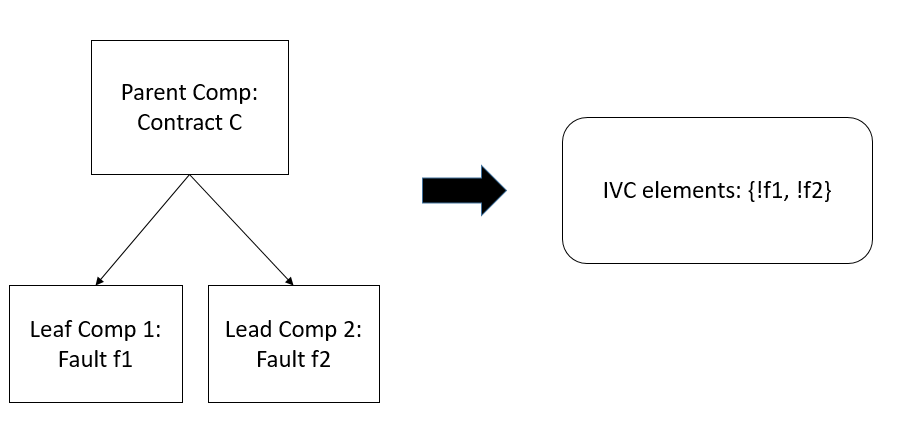
\includegraphics[scale=0.5]{images/ivcElements1.png}
	\caption{IVC Elements used for Consideration in a Leaf Layer of a System}
		\label{fig:ivcElements1}
	\end{center}
\end{figure}

Different layers of the architecture (and hence proof) provide slightly different information to the \aivcalg algorithm. This is ``given" to the IVC algorithm by the insertion of a Lustre statement with the keyword \texttt{\%IVC} followed by the fault activation literal. \\ \texttt{--\%IVC \_\_fault\_\_independently\_\_active\_\_sensor}\\

The constraints on that literal are given through the use of an assert statement in Lustre.\\ \texttt{assert (\_\_fault\_\_independently\_\_active\_\_sensor = false)}\\

The leaf nodes contribute only constrained faults to the IVC elements as shown in Figure~\ref{fig:ivcElements1}. In the non-leaf layers of the program, both contracts and constrained faults are considered as shown in Figure~\ref{fig:ivcElements2}. The reason for this is that the contracts are used to prove the properties at the next highest level and are necessary for the verification of the properties. The faults are used to provide safety pertinant information for the minimal cut sets. 

\begin{figure}[htbp]
	\hspace*{-2cm}
	\vspace{-0.1in} 
	\begin{center}
		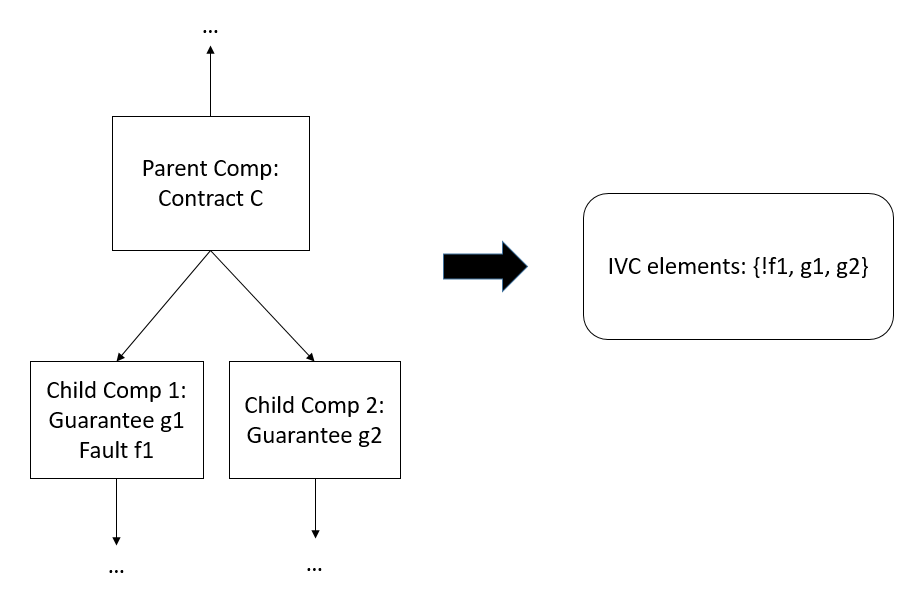
\includegraphics[scale=0.5]{images/ivcElements2.png}
	\caption{IVC Elements used for Consideration in a Middle Layer of a System}
		\label{fig:ivcElements2}
	\end{center}
\end{figure}

The all MIVCs algorithm returns the minimal set of these elements necessary to prove the properties. This equates to any contracts or inactive faults that must be present in order for the verification of properties in the model. From here, we perform a number of algorithms to transform all MIVCs into minimal cut sets.


%%%%%%%%%%%%%%%%%%%%%%%%%%%%%%%%%%%%%%%%%%%%%%%%%
%%%%%%%%%%%%%%%%%%%%            ALGORITHM DETAILS
\subsubsection{Algorithms}
The generation of \textit{MIVCs} traverses the program in a top down fashion. Likewise, the transformation of \textit{MIVCs} to MinCutSets traverses this program layer by layer if and only if all MIVCs have been generated. It is a requirement of the minimal hitting set algorithm that \textit{all} MUSs are used to find the MCSs~\cite{liffiton2016fast,gainer2017minimal,murakami2013efficient}. Thus, once all the MIVCs have been found and the minimal hitting set algorithm has completed, %our 
the MinCutSet Generation algorithm can begin. 

The MinCutSet Generation Algorithm begins with a list of MCSs specific to a top level property. These MCSs may contain a mixture of fault activation literals constrained to \textit{false} and %\textit{true} subcomponent contracts.
and subcomponent contracts constrained to \textit{true}. We remove all constraints from each MCS and call the resulting sets $I$, for \textit{Intermediate} set. Replacement of subcomponent contracts with their respective minimal cut sets can then proceed. For each of those contracts in $I$, we check to see if we have previously obtained a MinCutSet for that contract. If so, replacement is performed. If not, we recursively call this algorithm to obtain the list of all MinCutSets associated with this subcomponent contract. At a certain point, there will be no more contracts in the set $I$ in which case we have a minimal cut set for the current property. When this set is obtained, we store it in a lookup table keyed by the given property that this $I$ is associated with. 

A small example will illustrate this process. \danielle{Do I want to have a more concrete example? If so, pull from thesis proposal sensor example. If a shorter more abstract example is okay, do that.}







Algorithm~\ref{alg:generation_alg} describes this process.


\begin{algorithm}[htbp]
\SetKwFunction{FMain}{replace}
 \SetKwProg{Fn}{Function}{:}{}

	\Fn{\FMain{$P$}}{
		$List(I)$:= $List(MCS)$ for $P$ with all constraints removed \;
		\For{all $I \in List(I)$}{
			\eIf{there exists contracts $g \in I$}{
				\For{all constrained contracts $g \in I$}{
					\eIf{there exists $MinCutSets$ for $g$ in lookup table}{
						\For{all $minCut(g)$}{
							$I_{repl} = I$ \;
							$I_{repl} :=$ replace $g$ with $minCut(g)$ \;
							add $I_{repl}$ to $List(I)$ \;
						} %end for all cut sets of g
					}{
						replace($g$) \;
					} % end else if no cut sets in lookup table
				} % end for all constrained contracts in I
			}{
				add $I$ as $minCut(g)$ for $P$ \;
			} %end else if there exists contracts in I
		}%end for all I in list(I)
	}
%	\caption{Minimal Cut Set Generation Algorithm}
	\caption{MinCutSets Generation Algorithm}
	\label{alg:generation_alg}
\end{algorithm}

The number of replacements $R$ that are made in this algorithm are constrained by the number of minimal cut sets there are 
for all $\alpha$ contracts within the initial MCS. 

We call the set of all minimal cut sets for a contract $g$: $Cut(g)$. The following formula defines an upper bound on the number of replacements. The validity of this statement follows directly from the general multiplicative combinatorial principle. The number of replacements $R$ is bounded by the following formula:
\begin{equation}
\label{eq:bound}
  R \leq {\displaystyle \sum_{i=1}^{\alpha} }({\displaystyle \prod_{j=1}^{i} |Cut(g_j)|})  
\end{equation}


It is also important to note that the cardinality of $List(I)$ is bounded, i.e. the algorithm terminates. Every new $I$ that is generated through some replacement of a contract with its minimal cut set is added to $List(I)$ in order to continue the replacement process for all contracts in $I$. Adding to this set requires proof regarding termination.
\begin{theorem}
Algorithm~\ref{alg:generation_alg} terminates
\begin{proof}
No infinite sets are generated by the \aivcalg or minimal hitting set algorithms~\cite{Ghassabani2017EfficientGO,murakami2013efficient}; therefore, every MCS produced is finite. Thus, every $MinCutSet$ of every contract $g$ is finite. Furthermore, a bound exists on the number of additional intermediate sets $I$ that are added to $List(I)$: \\
$|List(I)| \leq R$ (Equation~\ref{eq:bound}).
\end{proof}
\end{theorem}

The reason for this upper bound is that for a contract $g_1$ in MCS, we make $|Cut(g_1)|$ replacements and add the resulting lists to $List(I)$. Then we move to the next contract $g_2$ in $I$. We must additionally make $|Cut(g_1)| \times |Cut(g_2)|$ replacements and add all of these resulting lists to $List(I)$, and so on throughout all contracts. Through the use of basic combinatorial principles, we end with the above formula for the upper bound on the number of additional intermediate sets.


\subsubsection{Pruning to Address Scalability}
The MinCutSets are filtered during this process based on a fault hypothesis given before analysis begins. The Safety Annex provides the capability to specify a type of verification in what is called a \textit{fault hypothesis statement}. These come in two forms: maximum number of faults or probabilistic analysis. Algorithm~\ref{alg:generation_alg} is the general approach, but the implementation changes slightly depending on which form of analysis is being performed. This pruning improves performance and diminishes the problem of combinatorial explosions in the size of minimal cut sets for larger models. \\

\textbf{Max $N$ Analysis Pruning} This statement restricts the number of faults that can be independently active simultaneously and verification is run with this restriction present. For example, if a max 2 fault hypothesis is specified, two or fewer faults may be active at once. In terms of minimal cut sets, this statement restricts the cardinality of minimal cut sets generated.

If the number of faults in an intermediate set $I$ exceeds the threshold $N$, any further replacement of remaining contracts in that intermediate set can never decrease the total number of faults in $I$; therefore, this intermediate set is eliminated from consideration.\\

\textbf{Probabilistic Analysis Pruning} The second type of hypothesis statement restricts the cut sets by use of a probabilistic threshold. Any cut sets with combined probability higher than the given probabilistic threshold are removed from consideration. The allowable combinations of faults are calculated before the transformation algorithm begins; this allows for a pruning of intermediate sets during the transformation. If the faults within an intermediate set are not a subset of any allowable combination, that intermediate set is pruned from consideration and no further replacements are made. 


 
    %\section{Preliminaries for Minimal Cut Set Generation}
\label{sec:prelimMCS}
In this research we consider \emph{safety properties} over infinite-state machines. The states are vectors of variables that define the values of state variables. We assume there are a set of legal \emph{initial states} and the safety property is specified as a formula over state variables. A \emph{reachable state space} means that all states are reachable from the initial state. 

Given a state space $U$, a transition system $(I,T)$ consists of an
initial state predicate $I : U \to \bool$ and a transition step
predicate $T : U \times U \to \bool$.
We define the notion of
reachability for $(I, T)$ as the smallest predicate $\reach : U \to
\bool$ which satisfies the following formulas:
\begin{gather*}
  \forall u.~ I(u) \Rightarrow \reach(u) \\
  \forall u, u'.~ \reach(u) \land T(u, u') \Rightarrow \reach(u')
\end{gather*}
A safety property $P : U \to \bool$ is a state predicate. A safety
property $P$ holds on a transition system $(I, T)$ if it holds on all
reachable states, i.e., $\forall u.~ \reach(u) \Rightarrow P(u)$,
written as $\reach \Rightarrow P$ for short. When this is the case, we
write $(I, T)\vdash P$.

\subsection{Induction}
For an arbitrary transition system $(I, T)$, computing reachability
can be very expensive or even impossible. Thus, we need a more
effective way of checking if a safety property $P$ is satisfied by the
system. The key idea is to over-approximate reachability. If we can
find an over-approximation that implies the property, then the
property must hold. Otherwise, the approximation needs to be refined.

A good first approximation for reachability is the property itself.
That is, we can check if the following formulas hold:
\begin{gather}
  \forall s.~ I(s) \Rightarrow P(s)
  \label{eq:1-ind-base} \\
  \forall s, s'.~ P(s) \land T(s, s') \Rightarrow P(s')
  \label{eq:1-ind-step}
\end{gather}
If both formulas hold then $P$ is {\em inductive} and holds over the
system. If (\ref{eq:1-ind-base}) fails to hold, then $P$ is violated
by an initial state of the system. If (\ref{eq:1-ind-step}) fails to
hold, then $P$ is too much of an over-approximation and needs to be
refined.

The JKind model checker used in this research uses {\em
  $k$-induction} which unrolls the property over $k$ steps of the
transition system. For example, 1-induction consists of formulas
(\ref{eq:1-ind-base}) and (\ref{eq:1-ind-step}) above, whereas
2-induction consists of the following formulas:
\begin{gather*}
\forall s.~ I(s) \Rightarrow P(s) \\
\forall s, s'.~ I(s) \land T(s, s') \Rightarrow P(s') \\
\forall s, s', s''.~ P(s) \land T(s, s') \land P(s') \land T(s',
  s'') \Rightarrow P(s'')
\end{gather*}
That is, there are two base step checks and one inductive step check.
In general, for an arbitrary $k$, $k$-induction consists of $k$
base step checks and one inductive step check as shown in
Figure~\ref{fig:k-induction} (the universal quantifiers on $s_i$ have
been elided for space). We say that a property is $k$-inductive if it
satisfies the $k$-induction constraints for the given value of $k$.
The hope is that the additional formulas in the antecedent of the
inductive step make it provable.

\begin{figure}
\begin{gather*}
I(s_0) \Rightarrow P(s_0) \\[-2pt]
%
\vdots \\[2pt]
%
I(s_0) \land T(s_0, s_1) \land \cdots \land T(s_{k-2}, s_{k-1})
\Rightarrow P(s_{k-1}) \\[2pt]
%
P(s_0) \land T(s_0, s_1) \land \cdots \land P(s_{k-1}) \land
T(s_{k-1}, s_k) \Rightarrow P(s_k)
\end{gather*}
\caption{$k$-induction formulas: $k$ base cases and one inductive
  step}
\label{fig:k-induction}
\end{figure}

In practice, inductive model checkers often use a combination of the
above techniques. Thus, a typical conclusion is of the form ``$P$ with
lemmas $L_1, \ldots, L_n$ is $k$-inductive''.

\subsection{The SAT Problem}
Boolean Satisfiability (SAT) solvers attempt to determine if there exists a total truth assignment to a given propositional formula, that evaluates to TRUE. Generally, a propositional formula is any combination of the disjunction and conjunction of literals (as an example, $a$ and $\neg a$ are literals). For a given unsatisfiable problem, solvers try to generate a proof of unsatisfiability; this is generally more useful than a proof of satisfiability. Such a proof is dependent on identifying a subset of clauses that make the problem unsatisfiable (UNSAT). 

SAT solvers in model checking work over a constraint system to determine satisfiability. A \textit{constraint system} $C$ is an ordered set of $n$ abstract constraints $\{C_1, C_2, ..., C_n\}$ over a set of variables. The constraint $C_i$ restricts the allowed assignments of these variables in some way~\cite{liffiton2016fast}. Given a constraint system, we require some method of determining, for any subset $S \subseteq C$, whether $S$ is \textit{satisfiable} (SAT) or \textit{unsatisfiable} (UNSAT). When a subset $S$ is SAT, this means that there exists an assignment allowed by all $C_i \in S$; when no such assignment exists, $S$ is considered UNSAT. 

There are several ways of translating a propositional formula into clauses such that satisfiability is preserved~\cite{een2003temporal}. By performing this translation, $k$-inductive model checkers are able to utilize parallel SAT-solving engines to glean information about the proof of a safety property at each inductive step. Expression of the base and induction steps of a temporal induction proof as SAT problems is straightforward. As an example, we look at an arbitrary base case from Figure~\ref{fig:k-induction}.

\begin{gather*}
I(s_0) \land T(s_0, s_1) \land \cdots \land T(s_{k-2}, s_{k-1})
\land \neg P(s_{k-1})
\end{gather*}

When proving correctness it is shown that the formulas are \emph{unsatisfiable}. If an $n^{th}$ inductive-step is unsatisfiable, that means following an $n$-step trace where the property holds, there exists no next state where it fails, i.e., the property $P$ is provable.




    %\section{Formalization of the Method}
\label{sec:formMCS}
\danielle{Section desperately needs figures of some kind to break up the text. Will try to make a few small ones of PWR example results.}
Compositional analysis proceeds from the top layer of the architecture down through the system model; faults are defined on leaf level components and guarantees are defined on all components. Due to the difference in analysis per layer, this section focuses on the formalism per layer type we are in. 

Given an initial state $I$ and a transition relation $T$ consisting of conjunctive constraints as defined in section~\ref{sec:prelim}. The nominal guarantees of the system, $G$, consist of conjunctive constraints $g \in G$. Given no faults, each $g$ is one of the transition constraints $T_i$ where:

\begin{gather}
T_n = g_1 \land  g_2 \land \cdots \land g_n
\label{eq:Tn}
\end{gather}

We assume the property holds of the nominal relation $(I,T_n) \vdash P$. Given that our focus is on safety analysis in the presence of faults, let the set of all faults in the system be  denoted as $F$. A fault $f \in F$ is a deviation from the normal constraint imposed by a guarantee. Any ``faults" in a mid-layer are simply violated guarantees, or deviations from normal behavior.

\subsection{Top Layer of Compositional Analysis}
Since faults are defined at leaf layers of the architecture, the top (and middle) layers only contain guarantees in the analysis. The \aivcalg algorithm collects all {\em minimal unsatisfiable subsets} (MUSs) of a given transition system in terms of the \textit{negation} of the top level property~\cite{Ghassabani2017EfficientGO,bendik2018online}. Formally, an MUS of a constraint system $C$ is a set $M \subseteq C$ such that $M$ is unsatisfiable and $\forall c \in M$ : $M \setminus \{c\}$ is satisfiable. The MUSs are the minimal explanation of the infeasibility of this constraint system; equivalently, these are the minimal sets of model elements necessary for proof of the safety property.

Returning to our running example, this can be illustrated by the following. Given the constraint system $C = \{G_p, G_t, G_r, \neg P\}$, a minimal explanation of the infeasability of this system is the set $\{G_p, G_t, G_r,\}$. If all three guarantees hold, then $P$ is provable. 

A related set is a {\em minimal correction set} (MCS); a MCS $M$ of a constraint system $C$ is a subset $M\subseteq C$ such that $C \setminus M$ is satisfiable and $\forall S \subset M$ : $C \setminus S$ is unsatisfiable. A MCS can be seen to ``correct'' the infeasability of the constraint system by the removal from $C$ the constraints found in an MCS.

In the case of an UNSAT system, we may ask: what will correct this unsatisfiability? Returning to the PWR example, we can find the MCSs of the top level constraint system: $MCS_1 = \{G_t\}$, $MCS_2 = \{G_p\}$, $MCS_3 = \{G_r\}$. If any single guarantee is violated, a shut down from that subsystem will not get sent when it should and the safety property $P$ will be violated. 

A duality exists between the MUSs of a constraint system and the MCSs as established by Reiter \cite{reiter1987theory}. This duality is defined in terms of \textit{Minimal Hitting Sets} (\textit{MHS}). A hitting set of a collection of sets $A$ is a set $H$ such that every set in $A$ is ``hit'' by $H$; $H$ contains at least one element from every set in $A$. Every MUS of a constraint system is a minimal hitting set of the system's MCSs, and likewise every MCS is a minimal hitting set of the system's MUSs~\cite{liffiton2016fast, reiter1987theory, de1987diagnosing}.

For the PWR top level constraint system, it can be seen that each of the MCSs intersected with the MUS is nonempty. And now we have the minimal set of guarantees for which, if violated, will cause $P$ to be unprovable. 

\subsection{Leaf Layer of Compositional Analysis}
The faults in the safety annex are defined on leaf level components. Thus, for the lowest analysis layer, we must take into consideration faults and the guarantees their activation may violate. A fault $f \in F$ is a deviation from the normal constraint imposed by a guarantee. For the purposes of this paper, each guarantee at the leaf layer of analysis has an associated fault. Without loss of generality, we associate a single fault and an associated fault probability with a guarantee. Each fault $f_i$ is associated with an \emph{activation literal}, $af_i$, that determines whether the fault is active or inactive. 

To consider the system under the presence of faults, consider a set $GF$ of modified guarantees in the presence of faults and let a mapping be defined from activation literals $af_i \in AF$ to these modified guarantees $gf_i \in GF$. 
\begin{center}
$\sigma : AF \rightarrow GF$ \\
$gf_i = \sigma(af_i) =$ if $af_i$ then $f_i$ else $g_i$
\label{eq:sigma}
\end{center}

The transition system is composed of the set of modified guarantees $GF$ and a set of conjunctions assigning each of the activation literals $af_i \in AF$ to false: 

\begin{gather}
T = gf_1 \land gf_2 \land \cdots \land gf_n \land \neg af_1 \land \neg af_2 \land \cdots \land \neg af_n
\label{eq:T}
\end{gather}

\begin{lemma} If $(I,T_n) \vdash P$ for $T_n$ defined in equation~\ref{eq:Tn}, then $(I,T) \vdash P$ for $T$ defined in equation~\ref{eq:T}.
\begin{proof}
By application of successive evaluations of $\sigma$ on each constrained activation literal $\neg af_i$, the result is immediate.
\end{proof}
\end{lemma}

Consider the elements of $T$ as a set $GF \cup AF$, where $GF$ are the potentially faulty guarantees and $AF$ consists of the activation literals that determine whether a guarantee is faulty. This is a set that is considered by a SAT-solver for satisfiability during the $k$-induction procedures. The posited problem is thus: $GF \land AF \land \neg P$ for the safety property in question. Recall, if this is an \emph{unsatisfiable} constraint system, then $(I,T) \vdash P$. On the other hand, if it is \emph{satisfiable}, then we know that given the constraints in $GF$ and $AF$, $P$ is not provable. These are the exact constraints we wish to find. 

Let us view this in terms of the PWR system example and focus on the temperature sensor subsystem. The safety property to be proved is $G_t$, the supporting guarantees are found in each of the three temperature sensors, $g_{ti}$. Faults $f_{ti}$ are defined for each sensor. The transition system is: 
\begin{gather*}
T = gf_{t1} \land gf_{t2} \land gf_{t3}  \land \neg af_{t1} \land \neg af_{t2} \land \neg af_{t3}
\end{gather*}

The MIVCs for this subsystem layer correspond to all pairwise combinations of constrained activation literals. Intuitively, if any two sensor faults do {\em not} occur, then two of the three sensor guarantees are not violated and the system responds appropriately to high temperature; therefore, $G_t$ is provable. 

The MCSs for this subsystem layer happen to also correspond to all pairwise combinations of constrained activation literals. If any two sensor faults {\em do} occur, then two of the three sensor guarantees will be violated and the system does not respond to high temperature as required. This would result in the inability to prove $G_t$. (Note: it is not always the case that the MCSs are the same as the MIVCs -- in this case it is due to majority voting on three sensors.)

\subsection{Transforming MCS into Minimal Cut Set}
The MCSs contain the information needed to find minimal cut sets, but their elements consist of constrained activation literals and/or guarantees. The link between the activation literals, faults, and guarantees is defined through $\sigma$ mapping (equation~\ref{eq:sigma}). At the leaf layer, only activation literals are found in MCSs and $\sigma$ must be applied to each element in an MCS to map back to the associated fault. Without loss of generality, let $MCS = \{af_1, \cdots, af_m\}$. Let $\sigma (MCS) = \{\sigma (\neg af_{1}), \cdots, \sigma (af_{m})\}$ be a mapping where MCS is a minimal correction set with regard to some property $G$ and $MCS  \subseteq AF$. \danielle{Question: Does minimality need its own proof?}

\begin{lemma} $\sigma (MCS)$ is a minimal cut set of $G$. 
\begin{proof}
Assume towards contradiction that $\sigma (MCS)$ is not a cut set of $G$. Then $gf_1 \land \cdots \land gf_n \land af_1 \cdots \land af_m \land \neg af_{k+1} \land \neg af_n \land \neg G$ is unsatisfiable. Thus, the \emph{true} activation literals do not affect the provability of $G$. This contradicts $C \setminus MCS$ is satisfiable. 
Minimality follows directly from the definition of MCS.
\end{proof}
\end{lemma}

In terms of the PWR example, the minimal cut sets for the temperature subsystem property $G_t$ consist of all pairwise faults on the temperature sensors; if any two faults occur on the sensors at the same time, we violate the temperature subsystem guarantee. 

Once these lower level minimal cut sets are generated, it is a matter of simple set replacement to find the higher level minimal cut sets. This can be easily seen in our example. An MCS at the top level has the element $G_t$. We systematically replace the contract with the faults that cause their violation. This results in three distinct minimal cut sets for $P$ from the temperature subsystem: $\{f_{t1}, f_{t2}\}, \{f_{t1}, f_{t3}, \{f_{t2}, f_{t3}$. All minimal cut sets for $P$ are given as similar pairwise combinations from each subsystem and total 9 for the entire system.

\danielle{Seems I need a theorem to round it out: that replacement will give min cut sets of safety property. Will think about how to formulate this.}



    %\section{Implementation and Algorithms}
\label{sec:algs}
The implementation of this idea requires changing what information the \aivcalg algorithm uses to complete the proofs and generate MUSs. At each layer of analysis, the \aivcalg algorithm views the model as a constraint system consisting of the negation of the property in question (guarantees at lower levels, top-level properties at the highest level), and the supporting guarantees/assumptions from the direct child level. The information provided to this algorithm changes slightly when performing the minimal cut set algorithms.

\subsubsection{Implementation}
In this approach, we use the all MIVCs algorithm and provide it a constraint system consisting of the negation of the top level safety property, the contracts of system components, as well as the faults in each layer constrained to false. It then collects the MUSs of this constraint system.

\begin{figure}[htbp]
	\hspace*{-2cm}
	\vspace{-0.1in} 
	\begin{center}
		\includegraphics[scale=0.5]{images/ivcElements1.png}
	\caption{IVC Elements used for Consideration in a Leaf Layer of a System}
		\label{fig:ivcElements1}
	\end{center}
\end{figure}

Different layers of the architecture (and hence proof) provide slightly different information to the \aivcalg algorithm. This is ``given" to the IVC algorithm by the insertion of a Lustre statement with the keyword \texttt{\%IVC} followed by the fault activation literal. \\ \texttt{--\%IVC \_\_fault\_\_independently\_\_active\_\_sensor}\\

The constraints on that literal are given through the use of an assert statement in Lustre.\\ \texttt{assert (\_\_fault\_\_independently\_\_active\_\_sensor = false)}\\

The leaf nodes contribute only constrained faults to the IVC elements as shown in Figure~\ref{fig:ivcElements1}. In the non-leaf layers of the program, both contracts and constrained faults are considered as shown in Figure~\ref{fig:ivcElements2}. The reason for this is that the contracts are used to prove the properties at the next highest level and are necessary for the verification of the properties. The faults are used to provide safety pertinant information for the minimal cut sets. 

\begin{figure}[htbp]
	\hspace*{-2cm}
	\vspace{-0.1in} 
	\begin{center}
		\includegraphics[scale=0.5]{images/ivcElements2.png}
	\caption{IVC Elements used for Consideration in a Middle Layer of a System}
		\label{fig:ivcElements2}
	\end{center}
\end{figure}

The all MIVCs algorithm returns the minimal set of these elements necessary to prove the properties. This equates to any contracts or inactive faults that must be present in order for the verification of properties in the model. From here, we perform a number of algorithms to transform all MIVCs into minimal cut sets.


%%%%%%%%%%%%%%%%%%%%%%%%%%%%%%%%%%%%%%%%%%%%%%%%%
%%%%%%%%%%%%%%%%%%%%            ALGORITHM DETAILS
\subsubsection{Algorithms}
The generation of \textit{MIVCs} traverses the program in a top down fashion. Likewise, the transformation of \textit{MIVCs} to MinCutSets traverses this program layer by layer if and only if all MIVCs have been generated. It is a requirement of the minimal hitting set algorithm that \textit{all} MUSs are used to find the MCSs~\cite{liffiton2016fast,gainer2017minimal,murakami2013efficient}. Thus, once all the MIVCs have been found and the minimal hitting set algorithm has completed, %our 
the MinCutSet Generation algorithm can begin. 

The MinCutSet Generation Algorithm begins with a list of MCSs specific to a top level property. These MCSs may contain a mixture of fault activation literals constrained to \textit{false} and %\textit{true} subcomponent contracts.
and subcomponent contracts constrained to \textit{true}. We remove all constraints from each MCS and call the resulting sets $I$, for \textit{Intermediate} set. Replacement of subcomponent contracts with their respective minimal cut sets can then proceed. For each of those contracts in $I$, we check to see if we have previously obtained a MinCutSet for that contract. If so, replacement is performed. If not, we recursively call this algorithm to obtain the list of all MinCutSets associated with this subcomponent contract. At a certain point, there will be no more contracts in the set $I$ in which case we have a minimal cut set for the current property. When this set is obtained, we store it in a lookup table keyed by the given property that this $I$ is associated with. 

A small example will illustrate this process. \danielle{Do I want to have a more concrete example? If so, pull from thesis proposal sensor example. If a shorter more abstract example is okay, do that.}







Algorithm~\ref{alg:generation_alg} describes this process.


\begin{algorithm}[htbp]
\SetKwFunction{FMain}{replace}
 \SetKwProg{Fn}{Function}{:}{}

	\Fn{\FMain{$P$}}{
		$List(I)$:= $List(MCS)$ for $P$ with all constraints removed \;
		\For{all $I \in List(I)$}{
			\eIf{there exists contracts $g \in I$}{
				\For{all constrained contracts $g \in I$}{
					\eIf{there exists $MinCutSets$ for $g$ in lookup table}{
						\For{all $minCut(g)$}{
							$I_{repl} = I$ \;
							$I_{repl} :=$ replace $g$ with $minCut(g)$ \;
							add $I_{repl}$ to $List(I)$ \;
						} %end for all cut sets of g
					}{
						replace($g$) \;
					} % end else if no cut sets in lookup table
				} % end for all constrained contracts in I
			}{
				add $I$ as $minCut(g)$ for $P$ \;
			} %end else if there exists contracts in I
		}%end for all I in list(I)
	}
%	\caption{Minimal Cut Set Generation Algorithm}
	\caption{MinCutSets Generation Algorithm}
	\label{alg:generation_alg}
\end{algorithm}

The number of replacements $R$ that are made in this algorithm are constrained by the number of minimal cut sets there are 
for all $\alpha$ contracts within the initial MCS. 

We call the set of all minimal cut sets for a contract $g$: $Cut(g)$. The following formula defines an upper bound on the number of replacements. The validity of this statement follows directly from the general multiplicative combinatorial principle. The number of replacements $R$ is bounded by the following formula:
\begin{equation}
\label{eq:bound}
  R \leq {\displaystyle \sum_{i=1}^{\alpha} }({\displaystyle \prod_{j=1}^{i} |Cut(g_j)|})  
\end{equation}


It is also important to note that the cardinality of $List(I)$ is bounded, i.e. the algorithm terminates. Every new $I$ that is generated through some replacement of a contract with its minimal cut set is added to $List(I)$ in order to continue the replacement process for all contracts in $I$. Adding to this set requires proof regarding termination.
\begin{theorem}
Algorithm~\ref{alg:generation_alg} terminates
\begin{proof}
No infinite sets are generated by the \aivcalg or minimal hitting set algorithms~\cite{Ghassabani2017EfficientGO,murakami2013efficient}; therefore, every MCS produced is finite. Thus, every $MinCutSet$ of every contract $g$ is finite. Furthermore, a bound exists on the number of additional intermediate sets $I$ that are added to $List(I)$: \\
$|List(I)| \leq R$ (Equation~\ref{eq:bound}).
\end{proof}
\end{theorem}

The reason for this upper bound is that for a contract $g_1$ in MCS, we make $|Cut(g_1)|$ replacements and add the resulting lists to $List(I)$. Then we move to the next contract $g_2$ in $I$. We must additionally make $|Cut(g_1)| \times |Cut(g_2)|$ replacements and add all of these resulting lists to $List(I)$, and so on throughout all contracts. Through the use of basic combinatorial principles, we end with the above formula for the upper bound on the number of additional intermediate sets.


\subsubsection{Pruning to Address Scalability}
The MinCutSets are filtered during this process based on a fault hypothesis given before analysis begins. The Safety Annex provides the capability to specify a type of verification in what is called a \textit{fault hypothesis statement}. These come in two forms: maximum number of faults or probabilistic analysis. Algorithm~\ref{alg:generation_alg} is the general approach, but the implementation changes slightly depending on which form of analysis is being performed. This pruning improves performance and diminishes the problem of combinatorial explosions in the size of minimal cut sets for larger models. \\

\textbf{Max $N$ Analysis Pruning} This statement restricts the number of faults that can be independently active simultaneously and verification is run with this restriction present. For example, if a max 2 fault hypothesis is specified, two or fewer faults may be active at once. In terms of minimal cut sets, this statement restricts the cardinality of minimal cut sets generated.

If the number of faults in an intermediate set $I$ exceeds the threshold $N$, any further replacement of remaining contracts in that intermediate set can never decrease the total number of faults in $I$; therefore, this intermediate set is eliminated from consideration.\\

\textbf{Probabilistic Analysis Pruning} The second type of hypothesis statement restricts the cut sets by use of a probabilistic threshold. Any cut sets with combined probability higher than the given probabilistic threshold are removed from consideration. The allowable combinations of faults are calculated before the transformation algorithm begins; this allows for a pruning of intermediate sets during the transformation. If the faults within an intermediate set are not a subset of any allowable combination, that intermediate set is pruned from consideration and no further replacements are made. 

\chapter{Case Studies}
\label{chap:caseStudies}

\section{Wheel Brake System}
\label{sec:wbs}
To demonstrate the fault modeling capabilities of the Safety Annex we will use the Wheel Brake System (WBS) described in AIR6110~\cite{AIR6110}.  This system is a well-known example that has been used as a case study for safety analysis, formal verification, and contract based design~\cite{DBLP:conf/cav/BozzanoCPJKPRT15, 10.1007/978-3-319-11936-6-7, CAV2015:BoCiGrMa, Joshi05:SafeComp}. The preliminary work for the Safety Annex was based on a simple model of the WBS~\cite{Stewart17:IMBSA}. To demonstrate a more complex fault modeling process, we constructed a functionally and structurally equivalent AADL version of the more complex WBS NuSMV/xSAP models~\cite{DBLP:conf/cav/BozzanoCPJKPRT15}.    

\begin{figure}[htbp]
	\centering
	\includegraphics[trim=0 9 0 5,clip,width=\textwidth]{images/wbs_arch4_diagram.pdf}
	\caption{Simplified Two-Wheel WBS}
	\label{fig:wbs}
\end{figure} 

The WBS is composed of two main parts: the Line Replaceable Unit control system and the electro-mechanical physical system.
The control system electronically controls the physical system and contains a redundant
channel of the Braking System Control Unit (BSCU) in case a detectable fault occurs in the active channel.
 It also commands antiskid braking. % in case of skidding on the ground. 
 The physical system consists of the hydraulic circuits running from hydraulic pumps to wheel brakes as well as valves that control the hydraulic fluid flow. This system provides braking force to each of the eight wheels of the aircraft. The wheels are all mechanically braked in pairs (one pair per landing gear). For simplicity, Figure~\ref{fig:wbs} displays only two of the eight wheels. 

There are three operating modes in the WBS model:

\begin{itemize}
	\renewcommand{\labelitemi}{\textbullet}
	\item In \textit{normal} mode, the system is composed of a \textit{green} hydraulic pump and one meter valve per each of the eight wheels. Each of the meter valves are controlled through electronic commands coming from the active channel of the BSCU. These signals provide braking and antiskid commands for each wheel. The braking command is determined through a sensor on the pedal and the antiskid command is determined by the \textit{Wheel Sensors}. 
	\item In \textit{alternate} mode, the system is composed of a \textit{blue} hydraulic pump, four meter valves, and four antiskid shutoff valves, one for each landing gear. The meter valves are mechanically commanded through the pilot pedal corresponding to each landing gear. If the selector detects lack of pressure in the green circuit, it switches to the blue circuit. 
	\item In \textit{emergency} mode, the system mode is entered if the \textit{blue} hydraulic pump fails. The accumulator pump has a reserve of pressurized hydraulic fluid and will supply this to the blue circuit in emergency mode. 
\end{itemize}

The WBS architecture model in AADL contains 30 different kinds of components, 169 component instances, and a model depth of 5 hierarchical levels. 

The behavioral model is encoded using the AGREE annex and the behavior is based on descriptions found in AIR6110. The top level system properties are given by the requirements and safety objectives in AIR6110. All of the subcomponent contracts support these system safety objectives through the use of assumptions on component input and guarantees on the output. 

An example system safety property is to ensure that there is no inadvertent braking of any of the wheels. This is based on a failure condition described in AIR6110 is \textit{Inadvertent wheel braking on one wheel during takeoff shall be less than 1E-9 per takeoff}. 
Inadvertent braking means that braking force is applied at the wheel but the pilot has not pressed the brake pedal.  In addition, the inadvertent braking requires that power and hydraulic pressure are both present, the plane is not stopped, and the wheel is rolling (not skidding). The property is stated in AGREE such that inadvertent braking does \textit{not} occur, as shown in Figure \ref{fig:inadvertent_braking}. 

\begin{figure}[htbp]
	%\vspace{-0.2in}
	\begin{center}
		\includegraphics[width=.7\textwidth]{images/inadvertent_braking.png}
	\end{center}
	\vspace{-0.3in}
	\caption{Safety Property: Inadvertent Braking}
	\label{fig:inadvertent_braking}
	%\vspace{-0.2in}
\end{figure}

\subsection{Nominal Model Analysis}
Before performing fault analysis, users should first check that the safety properties are satisfied by the nominal design model. This analysis can be performed monolithically or compositionally in AGREE. Using monolithic analysis, the contracts at the lower levels of the architecture are flattened and used in the proof of the top level safety properties of the system. Compositional analysis, on the other hand, will perform the proof layer by layer top down, essentially breaking the larger proof into subsets of smaller problems. For a more comprehensive description of these types of proofs and analyses, see additional publications related to AGREE \cite{cofer2012compositional,QFCS15:backes} and we refer you to Section~\ref{sec:concepts}.

The WBS has a total of 13 safety properties at the top level that are supported by subcomponent assumptions and guarantees. These are shown in Table \ref{tab:safetyProperties}. Given that there are 8 wheels, contract S18-WBS-0325-wheelX is repeated 8 times, one for each wheel. The behavioral model in total consists of over 440 assumptions and guarantees after instantiation.

\begin{table}[htbp]
\begin{center}
\begin{tabular}{@{}ll}
\toprule
\textbf{S18-WBS-R-0321} \\Loss of all wheel braking during landing or RTO shall be less than $5.0 \times 10^{-7}$ per flight.                                    \\ \midrule 
\textbf{S18-WBS-R/L-0322}  \\ Asymmetrical loss of wheel braking (Left/Right) shall be less than $5.0 \times 10^{-7}$ per flight. \\ \midrule
\textbf{S18-WBS-0323} \\ Never inadvertent braking with all wheels locked shall be less than $1.0 \times 10^{-9}$ per takeoff.                                                                                                                                                                                                               \\ \midrule
\textbf{S18-WBS-0324}  \\ Never inadvertent braking with all wheels shall be less than $1.0 \times 10^{-9}$ per takeoff.                                                                                                            \\ \midrule
\textbf{S18-WBS-0325-wheelX} \\ Never inadvertent braking of wheel X shall be less than $1.0 \times 10^{-9}$ per takeoff.                                                                                                           .                                                                                                                 \\ \bottomrule
\end{tabular}
\caption{Safety Properties of the WBS}
\label{tab:safetyProperties}
\end{center} 
\end{table} 


\subsection{Fault Model Analysis}
There are two main options for fault model analysis using the Safety Annex. The first option injects faults into the Lustre program based on the restrictions placed through the fault hypothesis. The bounded model checker engine used in JKind will find counterexamples to an invalid property. These counterexamples are returned to the user and include a trace of the system state that causes the violation. This includes any active faults that were part of that violation. The second option is used to generate minimal cut sets for the model. The fault activation literals and supporting guarantees are added to the MIVC algorithm elements as described in Sections~\ref{sec:formalization} and \ref{sec:impl}, the algorithm generating the cut sets is run (Section~\ref{sec:impl}), and the results are displayed to the user. 

\subsubsection{Verification in the Presence of Faults: Max \textit{n} Analysis}
Using a max number of faults for the hypothesis, the user can constrain the number of simultaneously active faults in the model. The faults are added to the AGREE model for the verification. Given the constraint on the number of possible simultaneously active faults, the model checker attempts to prove the top level properties given these constraints. If this cannot be done, the counterexample provided will show which of the faults ($n$ or less) are active and which contracts are violated. More detail on verification of fault models can be found in Section~\ref{sec:analysisResults}. 

The WBS was verified in the presence of faults given a \texttt{max 1 fault} hypothesis using compositional analysis. The time for complete model analysis was approximately 9 minutes, but a counterexample for certain top level properties took only around 20 seconds. (Recall that when using compositional verification in the presence of faults, that hypothesis applies to each layer separately -- the results are not rolled up as in the compositional generation of minimal cut sets. The counterexample given in this analysis pertains only to faults and contracts \textit{in a given layer}, and the timing of the counterexample reflects this single layer analysis result.) 

The verification in the presence of faults with \texttt{max 1 fault} hypothesis statement provided a counterexample to the property {\em S18-WBS-0325: never inadvertent braking of wheel i}, for $i = 1, \dots 8$. This property is given in Figure~\ref{fig:inadvertent_braking}. The intuition behind the failure is that the pedal was not pressed, the sensor stated that it was pressed, braking was commanded through the digital components, and brake pressure was supplied at the wheel. This sensor fault was a single point of failure with regard to all of the inadvertent braking properties. Later in this section we look at the sensor on the pedal position in closer detail from the lens of architectural design changes led by the analysis results. 

\subsubsection{Verification in the Presence of Faults: Probabilistic Analysis} 
Given a probabilistic fault hypothesis, this corresponds to performing analysis with the combinations of faults whose occurrence probability is less than the probability threshold. This is done by inserting assertions that allow those combinations in the Lustre code. If the model checker proves that the safety properties can be violated with any of those combinations, one of such combination will be shown in the counterexample. Probabilistic analysis done in this way must utilize the monolithic AGREE option. 

Recall that when using the \texttt{max 1 fault} hypothesis statement on the WBS, we found that the sensor was a single point of failure for multiple properties. The probability of this particular sensor failing is given in AIR6110~\cite{AIR6110} as $1.0 \times 10^{-2}$. The probabilistic hypothesis was set according to the thresholds given per property (see Table~\ref{tab:safetyProperties}) and the analysis was run monolithically on the WBS model. The total time {\em to generate a counterexample} for violated properties using a probabilistic hypothesis with monolithic analysis varied depending on the safety property; the range of times was between 15 seconds and 9 minutes. The property that took the longest to generate a counterexample for was {\em S18-WBS-0323: never inadvertent braking with all wheels locked shall be less than $1.0 \times 10^{-9}$ per takeoff.} The formula for this property references all 8 wheels and numerous subcomponents, most of which have faults associated with them. The low probability threshold combined with the formula complexity and the exponential increase in fault combinations likely served to make this the longest time in counterexample generation. For a full discussion on use of probabilistic thresholds in compositional analysis, see Section~\ref{sec:prob_generate}.

\subsubsection{Generate Minimal Cut Sets: Max \textit{n} Analysis}
\label{sec:maxN_generate}
As described in Section~\ref{sec:impl}, we use the \aivcalg algorithm to provide a full enumeration of all minimal set of model elements necessary for the proof of each top-level safety property in the model, and then transform all MIVCs into all minimal cut sets. In max $n$ analysis, the minimal cut sets are pruned to include only those with at cardinality less than or equal to the number $n$ specified in the fault hypothesis.

Generate minimal cut set analysis was performed on the Wheel Brake System and results are shown in Table~\ref{tab:wbs_maxN_results}. Notice in Table~\ref{tab:wbs_maxN_results}, the label across the top row refers to the cardinality (\textit{n}) and the corresponding column shows how many cut sets are generated of that cardinality. When the analysis is run, the user specifies the value \textit{n}. This gives cut sets of cardinality less than or equal to \textit{n}. Table~\ref{tab:wbs_maxN_results} shows the total number of cut sets of cardinality \textit{n}. The total number of cut sets computed at the given threshold is the sum across a row. (For the full text of the properties, see Table~\ref{tab:safetyProperties}.) 


\begin{table}[htbp]
\begin{center}
    \begin{tabular}{ | l | l | l | l | l | l |}
    \hline
    \textbf{Property} & $\bm{n = 1}$ & $\bm{n = 2}$ & $\bm{n = 3}$ & $\bm{n = 4}$ 
		& $\bm{n = 5}$    \\ \hline \hline
    0321 & 7 & 0 & 0 & 256 & 57,600   \\ \hline
    0322-R & 75 & 0 & 0 & 0 & 0  \\ \hline
    0322-L & 75 & 0 & 0 & 0 & 0  \\ \hline
    0323 & 182 & 0 & 0 & 0 & 0  \\ \hline
    0324 & 8 & 3,665 & 28,694 & 883,981 & - \\ \hline
    0325-WX & 33 & 0 & 0 &0 &0 \\ \hline
    \end{tabular}
    \caption{WBS Minimal Cut Set Results for Max \textit{n} Hypothesis}
    \label{tab:wbs_maxN_results}
    \end{center}
\end{table}


As can be seen in Table~\ref{tab:wbs_maxN_results}, the number of cut sets increases proportional to the cardinality of the cut sets. Intuitively, this can be understood as simple combinations of faults that can violate the hazard; if more things go wrong in a system at the same time, the more likely a property will be violated. Property S18-WBS-0324 with a max fault hypothesis of 5 was unable to finish due to an out of memory error. At the time that the error was thrown, the number of cut sets exceeded 1.5 million. In practice, it is not likely that an analyst will manually sift through a million or more cut sets, but rather will filter out the combinations that are sufficiently unlikely to occur. A probabilistic approach would be warranted in these situations. 

The next analysis shows the difference between the time it takes to generate all MIVCs and the time it takes to transform those MIVCs into minimal cut sets. Each column of Table~\ref{tab:wbs_mincut} labeled with the value of \textit{n} gives the fault hypothesis threshold for that analysis run. For comparison with the number of minimal cut sets generated per property, we refer to Table~\ref{tab:wbs_maxN_results}\footnote{The property S18-WBS-0325-WX is symmetric for all eight wheels. For readability, we only include wheel one verification timing results in Table~\ref{tab:wbs_mincut}. Likewise for property 0322-L/R.}.
\begin{table}[htbp]
\begin{center}
    \begin{tabular}{ | l | l | l | l | l | l | l |}
    \hline
    \textbf{Property} &  MIVC Gen & $n=1$ & $n=2$ & $n=3$ & $n=4$ & $n=5$     \\ \hline \hline
    0321 & 396.417 & 5.913 & 5.468 & 5.61 & 5.636 & 11.925  \\ \hline
    0322-L  & 407.078 & 5.931 & 5.435 & 5.302 & 5.268 & 5.243 \\ \hline
    0323 & 412.926 & 6.397 & 6.452 & 6.420  & 5.309 & 5.459\\ \hline
    0324 & 446.610 & 41.334 & 41.744 & 44.062 & 69.142 & -\\ \hline
    0325-W1 & 391.137 & 5.632 & 5.388 &5.359 &5.301 & 5.236 \\ \hline
    \end{tabular}
    \caption{WBS Analysis Time in Seconds}
    \label{tab:wbs_mincut}
    \end{center}
\end{table}
The overall time of the algorithms used for minimal cut set generation is quite small compared to the nominal analysis and extended model analysis time. This is not altogether surprising; the nominal and extended analysis is contending with an infinite state model checking problem whereas the algorithms presented to generate minimal cut sets deal with set element algorithms and boolean formula manipulation. The greatest time recorded was for property S18-WBS-0324 at $n = 4$; the reason is clear when comparing this with Table~\ref{tab:wbs_maxN_results}: the total number of minimal cut sets computed for this threshold is 916,349.  

\subsubsection{Generate Minimal Cut Sets: Probabilistic Analysis}
\label{sec:prob_generate}
Both probabilistic analysis and max $n$ analysis use the same underlying minimal cut set generation algorithm, but in probabilistic analysis the minimal cut sets are pruned to include only those fault combinations whose probability of simultaneous occurrence exceed the given threshold in the hypothesis. 

The probabilistic analysis for the WBS was given a top level threshold per property as stated in AIR6110 and shown in Table~\ref{tab:safetyProperties}. The faults associated with various components were all given probability of occurrence according to the AIR6110 document~\cite{AIR6110}. The table shows the property name and associated probability. The generation of minimal cut sets provided all sets that violate that property whose combined probabilities (assuming independence) are greater than the threshold. The number of sets per cardinality are listed in the table. 

\begin{table}[htbp]
\begin{center}
    \begin{tabular}{ | l | l | l | l | l | l | l | }
    \hline
    \textbf{Property} & $n=1$ & $n=2$ & $n=3$ & $n=4$ 
		& $n=5$    \\ \hline \hline
    0321: $5.0 \times 10^{-7}$ & 7 & 0 & 0 & 256 & 0   \\ \hline
    0322-R: $5.0 \times 10^{-7}$ & 75 & 0 & 0 &0 &0   \\ \hline
    0322-L: $5.0 \times 10^{-7}$ & 75 & 0 & 0 & 0 & 0    \\ \hline
    0323: $1.0 \times 10^{-9}$ & 182 & 0 & 0 & 0 & 0    \\ \hline
    0324: $1.0 \times 10^{-9}$ & 8 & 3665 & 0 & 0 & 0   \\ \hline
    0325-W1: $1.0 \times 10^{-9}$ & 33 & 0 & 0 &0 &0    \\ \hline
    \end{tabular}
    \caption{WBS Minimal Cut Set Results for Probabilistic Hypotheses}
    \label{tab:wbs_prob_results}
    \end{center}
\end{table}

As shown in Table~\ref{tab:wbs_prob_results}, the number of allowable combinations drops considerably when given probabilistic threshold as compared to just fault combinations of certain cardinalities. For example, one contract (inadvertent wheel braking of all wheels) had over a million minimal cut sets produced when looking at it in terms of max N analysis, but after taking probabilities into account, it is seen on Table~\ref{tab:wbs_prob_results} that the likely contributors to a hazard are minimal cut sets of cardinality one. The probabilistic analysis eliminated many thousands of cut sets from consideration. The total computation time for these runs is given in Table~\ref{tab:analysisTimeWBSProb}.


\begin{table}[htbp]
\begin{center}
    \begin{tabular}{ | l | l | l | l | l | l | l | }
    \hline
    \textbf{Property} & Total Analysis Time   \\ \hline \hline
    R-0321: $5.0 \times 10^{-7}$ & 433.144 sec  \\ \hline
    R-0322: $5.0 \times 10^{-7}$  & 431.954 sec  \\ \hline
    L-0322: $5.0 \times 10^{-7}$  & 429.081 sec    \\ \hline
    0323: $1.0 \times 10^{-9}$  & 571.216 sec    \\ \hline
    0324: $1.0 \times 10^{-9}$ & 589.07 sec   \\ \hline
    0325-W1: $1.0 \times 10^{-9}$ & 430.021 sec    \\ \hline
    \end{tabular}
    \caption{WBS Minimal Cut Set Time for Probabilistic Hypothesis}
    \label{tab:analysisTimeWBSProb}
    \end{center}
\end{table}


It is clear that the lower probabilistic threshold for properties 0323-0325-WX allowed more fault combinations to be possible which increased computation time. One must also recall property 0324 from the max \textit{n} analysis whose threshold of $n=4$ produced close to a million cut sets of various cardinalities. The pruning according to probabilities cut out many of these sets from consideration; they are sufficiently unlikely to occur together. 

\subsubsection{Display Results from Generate Minimal Cut Sets}
Results from Generate Minimal Cut Sets analysis can be represented in one of the following forms. 
\begin{enumerate}
\item The minimal cut sets can be presented in text form with the total number per property, cardinality of each, and description strings showing the property and fault information. A sample of this output is shown in Figure~\ref{fig:detailedMCS}. 
\begin{figure}[htbp]
	\hspace*{-2cm}
	\vspace{-0.1in} 
	\begin{center}
		\includegraphics[scale=0.7]{images/wbsMCSDesc.png}
	\caption{Detailed Output of Minimal Cut Sets}
		\label{fig:detailedMCS}
	\end{center}
\end{figure}

\item The minimal cut set information can be presented in tally form. This does not contain the fault information in detail, but instead gives only the tally of cut sets per property. This is useful in large models with many cut sets as it reduces the size of the text file. An example of this output type is seen in Figure~\ref{fig:tallyMCS}.
\begin{figure}[htbp]
	\hspace*{-2cm}
	\vspace{-0.1in} 
	\begin{center}
		\includegraphics[scale=0.7]{images/wbsMCSTally.png}
	\caption{Tally Output of Minimal Cut Sets}
		\label{fig:tallyMCS}
	\end{center}
\end{figure}

\end{enumerate}

\subsubsection{Use of Analysis Results to Drive Design Change}
\label{sec:designChange}
We use a single top level requirement of the WBS: {\em S18-WBS-0323: Never inadvertent braking with all wheels locked} to illustrate how Safety Annex can be used to detect design flaws and how faults can affect the behavior of the system. 

Upon running max $n$ compositional fault analysis with $n = 1$, a pedal sensor fault was shown to be a single point of failure for the inadvertent braking properties. 
\begin{figure}[htbp]
	%\vspace{-0.2in}
	\begin{center}
		\includegraphics[width=0.8\textwidth]{images/counterexample.png}
	\end{center}
	\vspace{-0.3in}
	\caption{Counterexample for Inadvertent Braking}
	\label{fig:counterexample}
	%\vspace{-0.2in}
\end{figure} 
A counterexample is shown in Figure \ref{fig:counterexample} showing the active fault on the pedal sensor. Depending on the goals of the system, the architecture currently modeled, and the mitigation strategies that are desired, various strategies are possible to mitigate the problem.

\begin{itemize}
\item Possible mitigation strategy 1: Monitor system can be added for the sensor: A monitor sub-component can be modeled in which it accesses the mechanical pedal as well as the signal from the sensor. If the monitor finds discrepancies between these values, it can send an indication of invalid sensor value to the top level of the system. In terms of the modeling, this would require a change to the behavioral contracts which use the sensor value. This validity would be taken into account through the means of $valid \land pedal\_sensor\_value$. 
%In the real system however, this mitigation would need to be taken into account. Whether this is a flag to the pilot who can then override the electrical system and switch to a different mode or perform some other action to mitigate the failed sensor must be discussed and implemented. 

\item Possible mitigation strategy 2: Redundancy can be added to the sensor: A sensor subsystem can be modeled which contains 3 or more sensors. The overall output from the sensor system may utilize a voting scheme to determine validity of sensor reading. There are multiple voting schemes that are possible, one of which is a majority voting (e.g. one sensor fails, the other two take majority vote and the correct value is passed). 
When three sensors are present, this mitigates the single point of failure problem. New behavioral contracts are added to the sensor system to model the behavior of redundancy and voting. 
\end{itemize}
\begin{figure}[htbp]
	%\vspace{-0.2in}
	\begin{center}
		\includegraphics[width=0.7\textwidth]{images/sensorsystem.png}
	\end{center}
	\vspace{-0.3in}
	\caption{Architectural Changes for Fault Mitigation}
	\label{fig:sensorsystem}
	%\vspace{-0.2in}
\end{figure}
In the case of the pedal sensor in the WBS, the latter of the two strategies outlined above was implemented. A sensor system was added to the model which held three pedal sensors. The output of this subsystem was constrained using a majority voting scheme. Upon subsequent runs of the analysis (regardless which type of run was used), resilience was confirmed in the system regarding the failure of a single pedal sensor. Figure \ref{fig:sensorsystem} outlines the architectural changes that were made in the model.

As can be seen through this single example, a system as large as the WBS would benefit from many iterations of this process. Furthermore, if the model is changed even slightly on the system development side, it would automatically be seen from the safety analysis perspective and any negative outcomes would be shown upon subsequent analysis runs. This effectively eliminates any miscommunications between the system development and analysis teams and creates a new safeguard regarding model changes. 

For more information on types of fault models that can be created as well as details on analysis results, see the users guide located in the GitHub repository \cite{SAGithub}. This repository also contains all models used in this project. 
\section{Process ID Example}
\label{sec:pid}
The illustration of asymmetric fault implementation can be seen through a simple example where 4 nodes report to each other their own process ID (PID). Each node has a 1-3 connection and thus each node is a candidate for an asymmetric fault. Given this architecture, a top level contract of the system is simply that all nodes report and see the correct PID of all other nodes. Naturally in the absence of faults, this holds. But when one asymmetric fault is introduced on any of the nodes, this contract cannot be verified. What is desired is a protocol in which all nodes agree on a value (correct or arbitrary) for all PIDs. 

\subsection{The Agreement Protocol Behavioral Implementation}
In order to mitigate this problem, special attention must be given to the behavioral model. Using the strategies outlined in previous research~\cite{bracha1987asynchronous,Driscoll-Byzantine-Fault}, the agreement protocol is specified in AGREE to create a model resilient to one active Byzantine fault. 

The objective of the agreement protocol is for all correct (non-failed) nodes to eventually reach agreement on the PID values of the other nodes. There are $n$ nodes, possibly $f$ failed nodes. The protocol requires $n > 3f$ nodes to handle a single fault. The point is to achieve distributed agreement and coordinated decisions.
The properties that must be verified in order to prove the protocol works as desired are as follows: 
\begin{itemize}
	\item All correct (non-failed) nodes eventually reach a decision regarding the value they have been given.  In this solution, nodes will agree in $f+1$ time steps or rounds of communication.   
	\item If the source node is correct, all other correct nodes agree on the value that was originally sent by the source.  
	\item If the source node is failed, all other nodes must agree on some predetermined default value.  
\end{itemize}

The updated architecture of the PID example is shown in Figure~\ref{fig:PIDArch}. 
\begin{figure}[!htb]
        \center{\includegraphics[width=\textwidth] {images/PIDArch.png}}
        \caption{\label{fig:PIDArch} Updated PID Example Architecture}
\end{figure}

Each node reports its own PID to all other nodes in the first round of communication. In the second round, each node informs the others what they saw in terms of %everyones
everyone's PIDs. %Thus, new connections are added for this second round of communication.
The outputs from a node are described in Figure~\ref{fig:NodeOutputsPID}. %\janet{The figure needs to be updated, as node 2 sends to node 1, 2, 3; and node 3 sends to node 1, 2, 4; and node 4 sends to node 1, 2, 3}
\begin{figure}[!htb]
        \center{\includegraphics[width=0.9\textwidth] {images/NodeOutputsPID.png}}
        \caption{\label{fig:NodeOutputsPID} Description of the Outputs of Each Node in the PID Example}
\end{figure}
%These new connections 
These outputs are modeled as a nested data implementation in AADL and each field corresponds to a PID from a node. The AADL code fragment defining this data implementation is shown in Figure~\ref{fig:PIDNodeData}.

\begin{figure}[!htb]
        \center{\includegraphics[width=0.7\textwidth] {images/PIDNodeData.png}}
        \caption{\label{fig:PIDNodeData} Data Implementation in AADL for Node Outputs}
\end{figure}

The fault definition for %that is inserted explicitly into the model is connected to 
each node's output and can effect the data fields arbitrarily. This is a nondeterministic fault in two ways. It is nondeterministic how many receiving nodes see incorrect values and it is nondeterministic how many of the data fields are affected by this fault. This can be accomplished through the fault definition shown in Figure~\ref{fig:PIDFaultNode} and the fault node definition in Figure~\ref{fig:PIDFaultDef}. 

\begin{figure}[!htb]
        \center{\includegraphics[width=0.9\textwidth] {images/PIDFaultNode.png}}
        \caption{\label{fig:PIDFaultNode} Fault Definition on Node Outputs for PID Example}
\end{figure}

\begin{figure}[!htb]
        \center{\includegraphics[width=0.9\textwidth] {images/PIDFaultDef.png}}
        \caption{\label{fig:PIDFaultDef} Fault Node Definition for PID Example}
\end{figure}

Once the fault model is in place, the implementation in AGREE of the agreement protocol is developed. As stated previously, there are two cases that must be considered in the contracts of this system. 
\begin{itemize}
	\item In the case of no active faults, all nodes must agree on the correct PID of all other nodes. 
	\item In the case of an active fault on a node, all non-failed nodes must agree on a PID for all other nodes. 
\end{itemize}

These requirements are encoded in AGREE through the use of the following contracts. Figure~\ref{fig:PIDContract1} and Figure~\ref{fig:PIDContract2} show example contracts regarding Node 1 PID. There are similar contracts for each node's PID. 
\begin{figure}[!htb]
        \center{\includegraphics[width=0.9\textwidth] {images/PIDContract1.png}}
        \caption{\label{fig:PIDContract1} Agreement Protocol Contract in AGREE for No Active Faults}
\end{figure}

\begin{figure}[!htb]
        \center{\includegraphics[width=0.9\textwidth] {images/PIDCOntract2.png}}
        \caption{\label{fig:PIDContract2} Agreement Protocol Contract in AGREE Regarding Non-failed Nodes}
\end{figure}


\textbf{Referencing Fault Activation Status}
To fully implement the agreement protocol, it must be possible to describe whether or not a component has failed; this is performed through the use of a \textit{fault activation statement}. The user first defines \textit{eq} variables in AGREE that will correspond to specific faults in components. Each of the \textit{eq} variables declared in AGREE (i.e., \textit{n1\_failed, n2\_failed, n3\_failed, n4\_failed}) is linked to the fault activation status of the \textit{Asym\_Fail\_Any\_PID\_To\_Any\_Value} fault defined in a node subcomponent instance of the %top level 
AADL system implementation (i.e., \textit{node1}, \textit{node2}, \textit{node3}, \textit{node4}). The fault activation statements for the PID example are shown in Figure~\ref{fig:PID_faultActivationStmt}.

\begin{figure}[!htb]
        \center{\includegraphics[width=0.9\textwidth] {images/PID_faultActivationStmt.png}}
        \caption{\label{fig:PID_faultActivationStmt} Fault Activation Statement in PID Example}
\end{figure}

\subsection{Nominal and Fault Model Analysis}
The nominal model verification shows that all properties are valid. Upon running verification in the presence of faults with maximum one active fault, the first four properties stating that all nodes agree on the correct value (Figure~\ref{fig:PIDContract1}) fail. This is expected since this property is specific to the case when no faults are present in the model. The remaining 4 top level properties (Figure~\ref{fig:PIDContract2}) state that all non-failed nodes reach agreement in two rounds of communication. These are verified valid when any one asymmetric fault is present. This shows that the agreement protocol was successful in eliminating a single point of asymmetric failure from the model. Furthermore, when changing the number of allowed faults to two, these properties do not hold. This is expected given the theoretical result that $3f+1$ nodes are required in order to be resilient to $f$ faults and that $f+1$ rounds of communication are needed for successful protocol implementation.

A summary of the results follows. 
\begin{itemize}
	\item Nominal model: All top level guarantees are verified. All nodes output the correct value and all agree. 
	\item Fault model with one active fault: The first four guarantees fail (when no fault is present, all nodes agree: shown in Figure~\ref{fig:PIDContract1}). This is expected if faults are present. The last four guarantees (all non-failed nodes agree) are verified as true with one active fault. 
	\item Fault model with two active faults: All 8 guarantees fail. This is expected since in order to be resilient up to two active faults ($f=2$), we would need $3f + 1 = 7$ nodes and $f+1 = 3$ rounds of communication. 
\end{itemize}

This example illustrates the correct handling of such faults and how to utilize the capabilities of the safety annex to model asymmetric failures and test that a system is resilient to such faults. 

    %\section{Wheel Brake System}
\label{sec:wbs}
To demonstrate the fault modeling capabilities of the Safety Annex we will use the Wheel Brake System (WBS) described in AIR6110~\cite{AIR6110}.  This system is a well-known example that has been used as a case study for safety analysis, formal verification, and contract based design~\cite{DBLP:conf/cav/BozzanoCPJKPRT15, 10.1007/978-3-319-11936-6-7, CAV2015:BoCiGrMa, Joshi05:SafeComp}. The preliminary work for the Safety Annex was based on a simple model of the WBS~\cite{Stewart17:IMBSA}. To demonstrate a more complex fault modeling process, we constructed a functionally and structurally equivalent AADL version of the more complex WBS NuSMV/xSAP models~\cite{DBLP:conf/cav/BozzanoCPJKPRT15}.    

\begin{figure}[htbp]
	\centering
	\includegraphics[trim=0 9 0 5,clip,width=\textwidth]{images/wbs_arch4_diagram.pdf}
	\caption{Simplified Two-Wheel WBS}
	\label{fig:wbs}
\end{figure} 

The WBS is composed of two main parts: the Line Replaceable Unit control system and the electro-mechanical physical system.
The control system electronically controls the physical system and contains a redundant
channel of the Braking System Control Unit (BSCU) in case a detectable fault occurs in the active channel.
 It also commands antiskid braking. % in case of skidding on the ground. 
 The physical system consists of the hydraulic circuits running from hydraulic pumps to wheel brakes as well as valves that control the hydraulic fluid flow. This system provides braking force to each of the eight wheels of the aircraft. The wheels are all mechanically braked in pairs (one pair per landing gear). For simplicity, Figure~\ref{fig:wbs} displays only two of the eight wheels. 

There are three operating modes in the WBS model:

\begin{itemize}
	\renewcommand{\labelitemi}{\textbullet}
	\item In \textit{normal} mode, the system is composed of a \textit{green} hydraulic pump and one meter valve per each of the eight wheels. Each of the meter valves are controlled through electronic commands coming from the active channel of the BSCU. These signals provide braking and antiskid commands for each wheel. The braking command is determined through a sensor on the pedal and the antiskid command is determined by the \textit{Wheel Sensors}. 
	\item In \textit{alternate} mode, the system is composed of a \textit{blue} hydraulic pump, four meter valves, and four antiskid shutoff valves, one for each landing gear. The meter valves are mechanically commanded through the pilot pedal corresponding to each landing gear. If the selector detects lack of pressure in the green circuit, it switches to the blue circuit. 
	\item In \textit{emergency} mode, the system mode is entered if the \textit{blue} hydraulic pump fails. The accumulator pump has a reserve of pressurized hydraulic fluid and will supply this to the blue circuit in emergency mode. 
\end{itemize}

The WBS architecture model in AADL contains 30 different kinds of components, 169 component instances, and a model depth of 5 hierarchical levels. 

The behavioral model is encoded using the AGREE annex and the behavior is based on descriptions found in AIR6110. The top level system properties are given by the requirements and safety objectives in AIR6110. All of the subcomponent contracts support these system safety objectives through the use of assumptions on component input and guarantees on the output. 

An example system safety property is to ensure that there is no inadvertent braking of any of the wheels. This is based on a failure condition described in AIR6110 is \textit{Inadvertent wheel braking on one wheel during takeoff shall be less than 1E-9 per takeoff}. 
Inadvertent braking means that braking force is applied at the wheel but the pilot has not pressed the brake pedal.  In addition, the inadvertent braking requires that power and hydraulic pressure are both present, the plane is not stopped, and the wheel is rolling (not skidding). The property is stated in AGREE such that inadvertent braking does \textit{not} occur, as shown in Figure \ref{fig:inadvertent_braking}. 

\begin{figure}[htbp]
	%\vspace{-0.2in}
	\begin{center}
		\includegraphics[width=.7\textwidth]{images/inadvertent_braking.png}
	\end{center}
	\vspace{-0.3in}
	\caption{Safety Property: Inadvertent Braking}
	\label{fig:inadvertent_braking}
	%\vspace{-0.2in}
\end{figure}

\subsection{Nominal Model Analysis}
Before performing fault analysis, users should first check that the safety properties are satisfied by the nominal design model. This analysis can be performed monolithically or compositionally in AGREE. Using monolithic analysis, the contracts at the lower levels of the architecture are flattened and used in the proof of the top level safety properties of the system. Compositional analysis, on the other hand, will perform the proof layer by layer top down, essentially breaking the larger proof into subsets of smaller problems. For a more comprehensive description of these types of proofs and analyses, see additional publications related to AGREE \cite{cofer2012compositional,QFCS15:backes} and we refer you to Section~\ref{sec:concepts}.

The WBS has a total of 13 safety properties at the top level that are supported by subcomponent assumptions and guarantees. These are shown in Table \ref{tab:safetyProperties}. Given that there are 8 wheels, contract S18-WBS-0325-wheelX is repeated 8 times, one for each wheel. The behavioral model in total consists of over 440 assumptions and guarantees after instantiation.

\begin{table}[htbp]
\begin{center}
\begin{tabular}{@{}ll}
\toprule
\textbf{S18-WBS-R-0321} \\Loss of all wheel braking during landing or RTO shall be less than $5.0 \times 10^{-7}$ per flight.                                    \\ \midrule 
\textbf{S18-WBS-R/L-0322}  \\ Asymmetrical loss of wheel braking (Left/Right) shall be less than $5.0 \times 10^{-7}$ per flight. \\ \midrule
\textbf{S18-WBS-0323} \\ Never inadvertent braking with all wheels locked shall be less than $1.0 \times 10^{-9}$ per takeoff.                                                                                                                                                                                                               \\ \midrule
\textbf{S18-WBS-0324}  \\ Never inadvertent braking with all wheels shall be less than $1.0 \times 10^{-9}$ per takeoff.                                                                                                            \\ \midrule
\textbf{S18-WBS-0325-wheelX} \\ Never inadvertent braking of wheel X shall be less than $1.0 \times 10^{-9}$ per takeoff.                                                                                                           .                                                                                                                 \\ \bottomrule
\end{tabular}
\caption{Safety Properties of the WBS}
\label{tab:safetyProperties}
\end{center} 
\end{table} 


\subsection{Fault Model Analysis}
There are two main options for fault model analysis using the Safety Annex. The first option injects faults into the Lustre program based on the restrictions placed through the fault hypothesis. The bounded model checker engine used in JKind will find counterexamples to an invalid property. These counterexamples are returned to the user and include a trace of the system state that causes the violation. This includes any active faults that were part of that violation. The second option is used to generate minimal cut sets for the model. The fault activation literals and supporting guarantees are added to the MIVC algorithm elements as described in Sections~\ref{sec:formalization} and \ref{sec:impl}, the algorithm generating the cut sets is run (Section~\ref{sec:impl}), and the results are displayed to the user. 

\subsubsection{Verification in the Presence of Faults: Max \textit{n} Analysis}
Using a max number of faults for the hypothesis, the user can constrain the number of simultaneously active faults in the model. The faults are added to the AGREE model for the verification. Given the constraint on the number of possible simultaneously active faults, the model checker attempts to prove the top level properties given these constraints. If this cannot be done, the counterexample provided will show which of the faults ($n$ or less) are active and which contracts are violated. More detail on verification of fault models can be found in Section~\ref{sec:analysisResults}. 

The WBS was verified in the presence of faults given a \texttt{max 1 fault} hypothesis using compositional analysis. The time for complete model analysis was approximately 9 minutes, but a counterexample for certain top level properties took only around 20 seconds. (Recall that when using compositional verification in the presence of faults, that hypothesis applies to each layer separately -- the results are not rolled up as in the compositional generation of minimal cut sets. The counterexample given in this analysis pertains only to faults and contracts \textit{in a given layer}, and the timing of the counterexample reflects this single layer analysis result.) 

The verification in the presence of faults with \texttt{max 1 fault} hypothesis statement provided a counterexample to the property {\em S18-WBS-0325: never inadvertent braking of wheel i}, for $i = 1, \dots 8$. This property is given in Figure~\ref{fig:inadvertent_braking}. The intuition behind the failure is that the pedal was not pressed, the sensor stated that it was pressed, braking was commanded through the digital components, and brake pressure was supplied at the wheel. This sensor fault was a single point of failure with regard to all of the inadvertent braking properties. Later in this section we look at the sensor on the pedal position in closer detail from the lens of architectural design changes led by the analysis results. 

\subsubsection{Verification in the Presence of Faults: Probabilistic Analysis} 
Given a probabilistic fault hypothesis, this corresponds to performing analysis with the combinations of faults whose occurrence probability is less than the probability threshold. This is done by inserting assertions that allow those combinations in the Lustre code. If the model checker proves that the safety properties can be violated with any of those combinations, one of such combination will be shown in the counterexample. Probabilistic analysis done in this way must utilize the monolithic AGREE option. 

Recall that when using the \texttt{max 1 fault} hypothesis statement on the WBS, we found that the sensor was a single point of failure for multiple properties. The probability of this particular sensor failing is given in AIR6110~\cite{AIR6110} as $1.0 \times 10^{-2}$. The probabilistic hypothesis was set according to the thresholds given per property (see Table~\ref{tab:safetyProperties}) and the analysis was run monolithically on the WBS model. The total time {\em to generate a counterexample} for violated properties using a probabilistic hypothesis with monolithic analysis varied depending on the safety property; the range of times was between 15 seconds and 9 minutes. The property that took the longest to generate a counterexample for was {\em S18-WBS-0323: never inadvertent braking with all wheels locked shall be less than $1.0 \times 10^{-9}$ per takeoff.} The formula for this property references all 8 wheels and numerous subcomponents, most of which have faults associated with them. The low probability threshold combined with the formula complexity and the exponential increase in fault combinations likely served to make this the longest time in counterexample generation. For a full discussion on use of probabilistic thresholds in compositional analysis, see Section~\ref{sec:prob_generate}.

\subsubsection{Generate Minimal Cut Sets: Max \textit{n} Analysis}
\label{sec:maxN_generate}
As described in Section~\ref{sec:impl}, we use the \aivcalg algorithm to provide a full enumeration of all minimal set of model elements necessary for the proof of each top-level safety property in the model, and then transform all MIVCs into all minimal cut sets. In max $n$ analysis, the minimal cut sets are pruned to include only those with at cardinality less than or equal to the number $n$ specified in the fault hypothesis.

Generate minimal cut set analysis was performed on the Wheel Brake System and results are shown in Table~\ref{tab:wbs_maxN_results}. Notice in Table~\ref{tab:wbs_maxN_results}, the label across the top row refers to the cardinality (\textit{n}) and the corresponding column shows how many cut sets are generated of that cardinality. When the analysis is run, the user specifies the value \textit{n}. This gives cut sets of cardinality less than or equal to \textit{n}. Table~\ref{tab:wbs_maxN_results} shows the total number of cut sets of cardinality \textit{n}. The total number of cut sets computed at the given threshold is the sum across a row. (For the full text of the properties, see Table~\ref{tab:safetyProperties}.) 


\begin{table}[htbp]
\begin{center}
    \begin{tabular}{ | l | l | l | l | l | l |}
    \hline
    \textbf{Property} & $\bm{n = 1}$ & $\bm{n = 2}$ & $\bm{n = 3}$ & $\bm{n = 4}$ 
		& $\bm{n = 5}$    \\ \hline \hline
    0321 & 7 & 0 & 0 & 256 & 57,600   \\ \hline
    0322-R & 75 & 0 & 0 & 0 & 0  \\ \hline
    0322-L & 75 & 0 & 0 & 0 & 0  \\ \hline
    0323 & 182 & 0 & 0 & 0 & 0  \\ \hline
    0324 & 8 & 3,665 & 28,694 & 883,981 & - \\ \hline
    0325-WX & 33 & 0 & 0 &0 &0 \\ \hline
    \end{tabular}
    \caption{WBS Minimal Cut Set Results for Max \textit{n} Hypothesis}
    \label{tab:wbs_maxN_results}
    \end{center}
\end{table}


As can be seen in Table~\ref{tab:wbs_maxN_results}, the number of cut sets increases proportional to the cardinality of the cut sets. Intuitively, this can be understood as simple combinations of faults that can violate the hazard; if more things go wrong in a system at the same time, the more likely a property will be violated. Property S18-WBS-0324 with a max fault hypothesis of 5 was unable to finish due to an out of memory error. At the time that the error was thrown, the number of cut sets exceeded 1.5 million. In practice, it is not likely that an analyst will manually sift through a million or more cut sets, but rather will filter out the combinations that are sufficiently unlikely to occur. A probabilistic approach would be warranted in these situations. 

The next analysis shows the difference between the time it takes to generate all MIVCs and the time it takes to transform those MIVCs into minimal cut sets. Each column of Table~\ref{tab:wbs_mincut} labeled with the value of \textit{n} gives the fault hypothesis threshold for that analysis run. For comparison with the number of minimal cut sets generated per property, we refer to Table~\ref{tab:wbs_maxN_results}\footnote{The property S18-WBS-0325-WX is symmetric for all eight wheels. For readability, we only include wheel one verification timing results in Table~\ref{tab:wbs_mincut}. Likewise for property 0322-L/R.}.
\begin{table}[htbp]
\begin{center}
    \begin{tabular}{ | l | l | l | l | l | l | l |}
    \hline
    \textbf{Property} &  MIVC Gen & $n=1$ & $n=2$ & $n=3$ & $n=4$ & $n=5$     \\ \hline \hline
    0321 & 396.417 & 5.913 & 5.468 & 5.61 & 5.636 & 11.925  \\ \hline
    0322-L  & 407.078 & 5.931 & 5.435 & 5.302 & 5.268 & 5.243 \\ \hline
    0323 & 412.926 & 6.397 & 6.452 & 6.420  & 5.309 & 5.459\\ \hline
    0324 & 446.610 & 41.334 & 41.744 & 44.062 & 69.142 & -\\ \hline
    0325-W1 & 391.137 & 5.632 & 5.388 &5.359 &5.301 & 5.236 \\ \hline
    \end{tabular}
    \caption{WBS Analysis Time in Seconds}
    \label{tab:wbs_mincut}
    \end{center}
\end{table}
The overall time of the algorithms used for minimal cut set generation is quite small compared to the nominal analysis and extended model analysis time. This is not altogether surprising; the nominal and extended analysis is contending with an infinite state model checking problem whereas the algorithms presented to generate minimal cut sets deal with set element algorithms and boolean formula manipulation. The greatest time recorded was for property S18-WBS-0324 at $n = 4$; the reason is clear when comparing this with Table~\ref{tab:wbs_maxN_results}: the total number of minimal cut sets computed for this threshold is 916,349.  

\subsubsection{Generate Minimal Cut Sets: Probabilistic Analysis}
\label{sec:prob_generate}
Both probabilistic analysis and max $n$ analysis use the same underlying minimal cut set generation algorithm, but in probabilistic analysis the minimal cut sets are pruned to include only those fault combinations whose probability of simultaneous occurrence exceed the given threshold in the hypothesis. 

The probabilistic analysis for the WBS was given a top level threshold per property as stated in AIR6110 and shown in Table~\ref{tab:safetyProperties}. The faults associated with various components were all given probability of occurrence according to the AIR6110 document~\cite{AIR6110}. The table shows the property name and associated probability. The generation of minimal cut sets provided all sets that violate that property whose combined probabilities (assuming independence) are greater than the threshold. The number of sets per cardinality are listed in the table. 

\begin{table}[htbp]
\begin{center}
    \begin{tabular}{ | l | l | l | l | l | l | l | }
    \hline
    \textbf{Property} & $n=1$ & $n=2$ & $n=3$ & $n=4$ 
		& $n=5$    \\ \hline \hline
    0321: $5.0 \times 10^{-7}$ & 7 & 0 & 0 & 256 & 0   \\ \hline
    0322-R: $5.0 \times 10^{-7}$ & 75 & 0 & 0 &0 &0   \\ \hline
    0322-L: $5.0 \times 10^{-7}$ & 75 & 0 & 0 & 0 & 0    \\ \hline
    0323: $1.0 \times 10^{-9}$ & 182 & 0 & 0 & 0 & 0    \\ \hline
    0324: $1.0 \times 10^{-9}$ & 8 & 3665 & 0 & 0 & 0   \\ \hline
    0325-W1: $1.0 \times 10^{-9}$ & 33 & 0 & 0 &0 &0    \\ \hline
    \end{tabular}
    \caption{WBS Minimal Cut Set Results for Probabilistic Hypotheses}
    \label{tab:wbs_prob_results}
    \end{center}
\end{table}

As shown in Table~\ref{tab:wbs_prob_results}, the number of allowable combinations drops considerably when given probabilistic threshold as compared to just fault combinations of certain cardinalities. For example, one contract (inadvertent wheel braking of all wheels) had over a million minimal cut sets produced when looking at it in terms of max N analysis, but after taking probabilities into account, it is seen on Table~\ref{tab:wbs_prob_results} that the likely contributors to a hazard are minimal cut sets of cardinality one. The probabilistic analysis eliminated many thousands of cut sets from consideration. The total computation time for these runs is given in Table~\ref{tab:analysisTimeWBSProb}.


\begin{table}[htbp]
\begin{center}
    \begin{tabular}{ | l | l | l | l | l | l | l | }
    \hline
    \textbf{Property} & Total Analysis Time   \\ \hline \hline
    R-0321: $5.0 \times 10^{-7}$ & 433.144 sec  \\ \hline
    R-0322: $5.0 \times 10^{-7}$  & 431.954 sec  \\ \hline
    L-0322: $5.0 \times 10^{-7}$  & 429.081 sec    \\ \hline
    0323: $1.0 \times 10^{-9}$  & 571.216 sec    \\ \hline
    0324: $1.0 \times 10^{-9}$ & 589.07 sec   \\ \hline
    0325-W1: $1.0 \times 10^{-9}$ & 430.021 sec    \\ \hline
    \end{tabular}
    \caption{WBS Minimal Cut Set Time for Probabilistic Hypothesis}
    \label{tab:analysisTimeWBSProb}
    \end{center}
\end{table}


It is clear that the lower probabilistic threshold for properties 0323-0325-WX allowed more fault combinations to be possible which increased computation time. One must also recall property 0324 from the max \textit{n} analysis whose threshold of $n=4$ produced close to a million cut sets of various cardinalities. The pruning according to probabilities cut out many of these sets from consideration; they are sufficiently unlikely to occur together. 

\subsubsection{Display Results from Generate Minimal Cut Sets}
Results from Generate Minimal Cut Sets analysis can be represented in one of the following forms. 
\begin{enumerate}
\item The minimal cut sets can be presented in text form with the total number per property, cardinality of each, and description strings showing the property and fault information. A sample of this output is shown in Figure~\ref{fig:detailedMCS}. 
\begin{figure}[htbp]
	\hspace*{-2cm}
	\vspace{-0.1in} 
	\begin{center}
		\includegraphics[scale=0.7]{images/wbsMCSDesc.png}
	\caption{Detailed Output of Minimal Cut Sets}
		\label{fig:detailedMCS}
	\end{center}
\end{figure}

\item The minimal cut set information can be presented in tally form. This does not contain the fault information in detail, but instead gives only the tally of cut sets per property. This is useful in large models with many cut sets as it reduces the size of the text file. An example of this output type is seen in Figure~\ref{fig:tallyMCS}.
\begin{figure}[htbp]
	\hspace*{-2cm}
	\vspace{-0.1in} 
	\begin{center}
		\includegraphics[scale=0.7]{images/wbsMCSTally.png}
	\caption{Tally Output of Minimal Cut Sets}
		\label{fig:tallyMCS}
	\end{center}
\end{figure}

\end{enumerate}

\subsubsection{Use of Analysis Results to Drive Design Change}
\label{sec:designChange}
We use a single top level requirement of the WBS: {\em S18-WBS-0323: Never inadvertent braking with all wheels locked} to illustrate how Safety Annex can be used to detect design flaws and how faults can affect the behavior of the system. 

Upon running max $n$ compositional fault analysis with $n = 1$, a pedal sensor fault was shown to be a single point of failure for the inadvertent braking properties. 
\begin{figure}[htbp]
	%\vspace{-0.2in}
	\begin{center}
		\includegraphics[width=0.8\textwidth]{images/counterexample.png}
	\end{center}
	\vspace{-0.3in}
	\caption{Counterexample for Inadvertent Braking}
	\label{fig:counterexample}
	%\vspace{-0.2in}
\end{figure} 
A counterexample is shown in Figure \ref{fig:counterexample} showing the active fault on the pedal sensor. Depending on the goals of the system, the architecture currently modeled, and the mitigation strategies that are desired, various strategies are possible to mitigate the problem.

\begin{itemize}
\item Possible mitigation strategy 1: Monitor system can be added for the sensor: A monitor sub-component can be modeled in which it accesses the mechanical pedal as well as the signal from the sensor. If the monitor finds discrepancies between these values, it can send an indication of invalid sensor value to the top level of the system. In terms of the modeling, this would require a change to the behavioral contracts which use the sensor value. This validity would be taken into account through the means of $valid \land pedal\_sensor\_value$. 
%In the real system however, this mitigation would need to be taken into account. Whether this is a flag to the pilot who can then override the electrical system and switch to a different mode or perform some other action to mitigate the failed sensor must be discussed and implemented. 

\item Possible mitigation strategy 2: Redundancy can be added to the sensor: A sensor subsystem can be modeled which contains 3 or more sensors. The overall output from the sensor system may utilize a voting scheme to determine validity of sensor reading. There are multiple voting schemes that are possible, one of which is a majority voting (e.g. one sensor fails, the other two take majority vote and the correct value is passed). 
When three sensors are present, this mitigates the single point of failure problem. New behavioral contracts are added to the sensor system to model the behavior of redundancy and voting. 
\end{itemize}
\begin{figure}[htbp]
	%\vspace{-0.2in}
	\begin{center}
		\includegraphics[width=0.7\textwidth]{images/sensorsystem.png}
	\end{center}
	\vspace{-0.3in}
	\caption{Architectural Changes for Fault Mitigation}
	\label{fig:sensorsystem}
	%\vspace{-0.2in}
\end{figure}
In the case of the pedal sensor in the WBS, the latter of the two strategies outlined above was implemented. A sensor system was added to the model which held three pedal sensors. The output of this subsystem was constrained using a majority voting scheme. Upon subsequent runs of the analysis (regardless which type of run was used), resilience was confirmed in the system regarding the failure of a single pedal sensor. Figure \ref{fig:sensorsystem} outlines the architectural changes that were made in the model.

As can be seen through this single example, a system as large as the WBS would benefit from many iterations of this process. Furthermore, if the model is changed even slightly on the system development side, it would automatically be seen from the safety analysis perspective and any negative outcomes would be shown upon subsequent analysis runs. This effectively eliminates any miscommunications between the system development and analysis teams and creates a new safeguard regarding model changes. 

For more information on types of fault models that can be created as well as details on analysis results, see the users guide located in the GitHub repository \cite{SAGithub}. This repository also contains all models used in this project. 
    %\section{Process ID Example}
\label{sec:pid}
The illustration of asymmetric fault implementation can be seen through a simple example where 4 nodes report to each other their own process ID (PID). Each node has a 1-3 connection and thus each node is a candidate for an asymmetric fault. Given this architecture, a top level contract of the system is simply that all nodes report and see the correct PID of all other nodes. Naturally in the absence of faults, this holds. But when one asymmetric fault is introduced on any of the nodes, this contract cannot be verified. What is desired is a protocol in which all nodes agree on a value (correct or arbitrary) for all PIDs. 

\subsection{The Agreement Protocol Behavioral Implementation}
In order to mitigate this problem, special attention must be given to the behavioral model. Using the strategies outlined in previous research~\cite{bracha1987asynchronous,Driscoll-Byzantine-Fault}, the agreement protocol is specified in AGREE to create a model resilient to one active Byzantine fault. 

The objective of the agreement protocol is for all correct (non-failed) nodes to eventually reach agreement on the PID values of the other nodes. There are $n$ nodes, possibly $f$ failed nodes. The protocol requires $n > 3f$ nodes to handle a single fault. The point is to achieve distributed agreement and coordinated decisions.
The properties that must be verified in order to prove the protocol works as desired are as follows: 
\begin{itemize}
	\item All correct (non-failed) nodes eventually reach a decision regarding the value they have been given.  In this solution, nodes will agree in $f+1$ time steps or rounds of communication.   
	\item If the source node is correct, all other correct nodes agree on the value that was originally sent by the source.  
	\item If the source node is failed, all other nodes must agree on some predetermined default value.  
\end{itemize}

The updated architecture of the PID example is shown in Figure~\ref{fig:PIDArch}. 
\begin{figure}[!htb]
        \center{\includegraphics[width=\textwidth] {images/PIDArch.png}}
        \caption{\label{fig:PIDArch} Updated PID Example Architecture}
\end{figure}

Each node reports its own PID to all other nodes in the first round of communication. In the second round, each node informs the others what they saw in terms of %everyones
everyone's PIDs. %Thus, new connections are added for this second round of communication.
The outputs from a node are described in Figure~\ref{fig:NodeOutputsPID}. %\janet{The figure needs to be updated, as node 2 sends to node 1, 2, 3; and node 3 sends to node 1, 2, 4; and node 4 sends to node 1, 2, 3}
\begin{figure}[!htb]
        \center{\includegraphics[width=0.9\textwidth] {images/NodeOutputsPID.png}}
        \caption{\label{fig:NodeOutputsPID} Description of the Outputs of Each Node in the PID Example}
\end{figure}
%These new connections 
These outputs are modeled as a nested data implementation in AADL and each field corresponds to a PID from a node. The AADL code fragment defining this data implementation is shown in Figure~\ref{fig:PIDNodeData}.

\begin{figure}[!htb]
        \center{\includegraphics[width=0.7\textwidth] {images/PIDNodeData.png}}
        \caption{\label{fig:PIDNodeData} Data Implementation in AADL for Node Outputs}
\end{figure}

The fault definition for %that is inserted explicitly into the model is connected to 
each node's output and can effect the data fields arbitrarily. This is a nondeterministic fault in two ways. It is nondeterministic how many receiving nodes see incorrect values and it is nondeterministic how many of the data fields are affected by this fault. This can be accomplished through the fault definition shown in Figure~\ref{fig:PIDFaultNode} and the fault node definition in Figure~\ref{fig:PIDFaultDef}. 

\begin{figure}[!htb]
        \center{\includegraphics[width=0.9\textwidth] {images/PIDFaultNode.png}}
        \caption{\label{fig:PIDFaultNode} Fault Definition on Node Outputs for PID Example}
\end{figure}

\begin{figure}[!htb]
        \center{\includegraphics[width=0.9\textwidth] {images/PIDFaultDef.png}}
        \caption{\label{fig:PIDFaultDef} Fault Node Definition for PID Example}
\end{figure}

Once the fault model is in place, the implementation in AGREE of the agreement protocol is developed. As stated previously, there are two cases that must be considered in the contracts of this system. 
\begin{itemize}
	\item In the case of no active faults, all nodes must agree on the correct PID of all other nodes. 
	\item In the case of an active fault on a node, all non-failed nodes must agree on a PID for all other nodes. 
\end{itemize}

These requirements are encoded in AGREE through the use of the following contracts. Figure~\ref{fig:PIDContract1} and Figure~\ref{fig:PIDContract2} show example contracts regarding Node 1 PID. There are similar contracts for each node's PID. 
\begin{figure}[!htb]
        \center{\includegraphics[width=0.9\textwidth] {images/PIDContract1.png}}
        \caption{\label{fig:PIDContract1} Agreement Protocol Contract in AGREE for No Active Faults}
\end{figure}

\begin{figure}[!htb]
        \center{\includegraphics[width=0.9\textwidth] {images/PIDCOntract2.png}}
        \caption{\label{fig:PIDContract2} Agreement Protocol Contract in AGREE Regarding Non-failed Nodes}
\end{figure}


\textbf{Referencing Fault Activation Status}
To fully implement the agreement protocol, it must be possible to describe whether or not a component has failed; this is performed through the use of a \textit{fault activation statement}. The user first defines \textit{eq} variables in AGREE that will correspond to specific faults in components. Each of the \textit{eq} variables declared in AGREE (i.e., \textit{n1\_failed, n2\_failed, n3\_failed, n4\_failed}) is linked to the fault activation status of the \textit{Asym\_Fail\_Any\_PID\_To\_Any\_Value} fault defined in a node subcomponent instance of the %top level 
AADL system implementation (i.e., \textit{node1}, \textit{node2}, \textit{node3}, \textit{node4}). The fault activation statements for the PID example are shown in Figure~\ref{fig:PID_faultActivationStmt}.

\begin{figure}[!htb]
        \center{\includegraphics[width=0.9\textwidth] {images/PID_faultActivationStmt.png}}
        \caption{\label{fig:PID_faultActivationStmt} Fault Activation Statement in PID Example}
\end{figure}

\subsection{Nominal and Fault Model Analysis}
The nominal model verification shows that all properties are valid. Upon running verification in the presence of faults with maximum one active fault, the first four properties stating that all nodes agree on the correct value (Figure~\ref{fig:PIDContract1}) fail. This is expected since this property is specific to the case when no faults are present in the model. The remaining 4 top level properties (Figure~\ref{fig:PIDContract2}) state that all non-failed nodes reach agreement in two rounds of communication. These are verified valid when any one asymmetric fault is present. This shows that the agreement protocol was successful in eliminating a single point of asymmetric failure from the model. Furthermore, when changing the number of allowed faults to two, these properties do not hold. This is expected given the theoretical result that $3f+1$ nodes are required in order to be resilient to $f$ faults and that $f+1$ rounds of communication are needed for successful protocol implementation.

A summary of the results follows. 
\begin{itemize}
	\item Nominal model: All top level guarantees are verified. All nodes output the correct value and all agree. 
	\item Fault model with one active fault: The first four guarantees fail (when no fault is present, all nodes agree: shown in Figure~\ref{fig:PIDContract1}). This is expected if faults are present. The last four guarantees (all non-failed nodes agree) are verified as true with one active fault. 
	\item Fault model with two active faults: All 8 guarantees fail. This is expected since in order to be resilient up to two active faults ($f=2$), we would need $3f + 1 = 7$ nodes and $f+1 = 3$ rounds of communication. 
\end{itemize}

This example illustrates the correct handling of such faults and how to utilize the capabilities of the safety annex to model asymmetric failures and test that a system is resilient to such faults. 

\chapter{Granularity of Specificationss}
\label{chap:granularity}
The specification of requirements is an important part the development of critical systems, and the analysis results are greatly dependent upon these specifications. Formal specification, as described in Section~\ref{sec:formalSpec}, is the translation of the informal system requirements into a mathematical logic to determine if the system design is correct~\cite{hinchey2012industrial}. The informal system requirements are often initially developed and written in natural language which is often ambiguous and always mathematically informal. The formal semantics of specified properties, such as LTL, is fully defined and thus is tractable to mathematical reasoning; this does not imply that formalization is fool-proof or straightforward to do~\cite{kotonya1998requirements}. 

 In the approach of system development and safety assessment of models that we describe in this research, we define these specifications in the form of \emph{guarantees} of the behavior of components and \emph{assumptions} regarding the environment. The verification task is to show that a system guarantee $P_s$ is provable given the behavior of its subcomponents $C_s$ and the system assumption $A_s$. A systems engineer must translate natural language requirements into these formal contracts for each component. If there are dependencies between contracts or irrelevant subexpressions within the statements, this may change the analysis results. 
 
The reason this is of interest to us is due to the use of MIVCs in the generation of minimal cut sets. Previous work has shown that the specification and formulation of the guarantees can affect the IVC analysis results~\cite{ghassabani_2018}. The algorithm used to generate the cut sets based on MIVC results may lead to the loss of minimality with regard to the cut set.  Assume that there is a single critical guarantee $g$ that is required to prove a safety property. This will be in the MIVC generation and the associated fault activation literal will be in the cut set. Assume the structure of the guarantee is $g = A \land B$ for Boolean formulae $A$ and $B$. There are also two leaf level faults, one that affects the truth value of $A$ and one that affects $B$. Of course either will violate the guarantee -- and hence be in the cut set, but if only $A$ is needed for the proof of the property, there will be more faults in the cut set than minimality suggests. 

To address this problem, we begin the exploration of granularity and automated methods to solve this problem. This chapter outlines our exploration into this topic. 

\section{Background Research and Foundation}
As described in Chapter~\ref{chap:prelim}, a transition relation is considered to be a conjunction of Boolean formulas. Depending on how contracts are specified in the model, it is possible to have a ``complete" specification, i.e., all of the equations in the model are required to determine the validity of the property. However, in certain cases, subexpressions of equations may be irrelevant. If the equation is decomposed into smaller pieces, this incompleteness becomes visible and the model is no longer completely {\em covered}. Simply put, coverage is a metric that determines how well properties cover the design of a model. It is often the case that splitting an equation of the model into more conjuncts, or equivalently, making the model more \textit{granular}, leads to lower coverage of the model. 

This can be seen in the IVCs generated for a given safety property. The intuition can be illustrated with a small example. If the safety property is: $P : A $ for some complex formula $A$ and an equation in the model is $g: A \land (B \lor C)$, the supporting equation $g$ will be an IVC. But $g$ also contains other statements that do not necessarily support the proof of $P$ -- the only portion of $g$ that matters to the proof is $A$. The IVCs in a more granular model would theoretically reflect only the necessary equations required for property verification, and thus would provide more specific analysis results. A more granular model in this small example could be $g_1 : A$ and $g_2: B \lor C$. Then we would see only $g_1$ in the IVC elements for $P$. 

Interestingly, similar work from a varied perspective has been done in test case generation, specifically \emph{Modified Condition and Decision Coverage} (MC/DC). It was found that MC/DC over implementations with structurally complex Boolean expressions are generally larger and more effective than MC/DC over functionally equivalent but structurally simpler implementations~\cite{gay2016effect}. An automated technique called \emph{inlining} provides a restructuring of the model by inlining simpler Boolean expressions into a single, now more complex, expression. An example of an unlined implementation is: 

\begin{figure}[h]
	\begin{center}
		\includegraphics[scale=1.0]{images/uninlinedEx.PNG}
	\end{center}
	\vspace{-1.5em}
	%\caption{Uninlined implementation example}
	%\label{fig:uninlined}
\end{figure}

And the associated inlined implementation is: 

\begin{figure}[h]
	\begin{center}
		\includegraphics[scale=1.0]{images/inlined.PNG}
	\end{center}
	\vspace{-1.5em}
	%%\caption{Inlined implementation example}
%	\label{fig:inlined}
\end{figure}

Inlining results in a behaviorally equivalent implementation with different structure (syntax). The reason MC/DC provides much greater coverage in terms of test case generation is because MC/DC on an inlined system will require specific combinations of input that will not be required to achieve coverage of the noninlined system~\cite{gay2016effect}. 

Inductive validity cores, on the other hand, attempt to answer a different kind of question about the model than test coverage. In the IVC case, the goal is to find the minimal sets of model elements that contribute to a proof of a safety property. When these model elements are pulled from the model in terms of guarantees and assumptions, the \emph{granularity} of these logical statements matters in the opposite way. The IVC algorithm performs no deeper traces than those defined in those model elements (guarantees/assumptions). For our purposes, it is beneficial at times to see which \emph{parts} of the contract are necessary for the proof. In this case, instead of making the contracts more complex (inlining), we wish to simplify the contracts (un-inlining). In this way, the IVCs are more specific with regard to which parts of the contract are vital to the proof. This will theoretically decompose the contracts and eliminate property dependencies within the model. 

Granularity of contracts for IVCs has been briefly discussed by Ghassabani~\cite{ghassabani_2018}, but to our knowledge has not been discussed in any other previous work -- in particular related to minimal cut set generation. Since IVC generation is a required first step of our minimal cut set algorithms, it is important to discuss how the granularity of the model will affect the cut sets generated through this approach. 

As described in Chapter~\ref{chap:mcsGen}, the backend model checker used in this transformation is \jkind which performs $k$-induction over a transition system defined with a Lustre program. Ghassabani performed a preliminary investigation of granularity within the context of the Lustre language. Lustre provides an adequate formalism for this discussion because it is top-level conjunctive, equational, and \textit{referentially transparent}~\cite{Halbwachs91:IEEE}. This means that the behavior of a Lustre program is defined by a system of equations and any subexpression on the right side of an equation can be extracted and assigned a fresh variable\footnote{A fresh variable is a variable with an identifier that has not been used within the program.} which is substituted into the original equation without changing the meaning of the program. In this context, \textit{granular refinement} is defined as an extraction of a subexpression into a new equation assigning a fresh variable. 


\section{Illustrative Example Showing the Effects of Granularity}
To see how different representations of the system will alter the IVC and MinCutSet computations, let us examine a simple sensor example system. In this simple AADL architecture, the environmental temperature and pressure is sent to a subsystem of sensors which contains a temp sensor and a pressure sensor, both of which receive the respective environmental inputs. If the temperature (or pressure) surpasses a given threshold, then the temp (pressure) sensor outputs a HIGH\_LEVELS flag. It also outputs the temperature (pressure) reading seen at the sensor. A diagram showing the two levels of the AADL implementation is shown in Figure~\ref{fig:sensorGran1}.  

\begin{figure}[h]
\begin{center}
\includegraphics[width=14cm]{images/sensorGran.png}
\caption{Tempurature Sensor System} 
\label{fig:sensorGran1}
\end{center}
\end{figure}

Now that the basic architecture is in place, we focus our attention on the requirements of each component. The behavior we wish to enforce at the temperature sensor level corresponds to the following two guarantees, $G_1$ and $G_2$. (Note: pressure sensor behavior is quite similar and for this reason, we will stick to the temperature for this example.) 

$G_1$: If environmental temperature surpasses threshold, then output high temperature indication: \textit{(temp $>$ THRESHOLD) $\implies$ (high\_temp\_indicator)}

$G_2$: Temperature read is equivalent to temperature in\footnote{This example eliminated the possibility of noise in the temp reading for simplicity's sake.}: \textit{temp = temp\_reading} 


These can be seen in the model as two distinct guarantees over the output of the sensor component. Now, as the contracts work their way up the system, there are distinct ways of writing them. For this, we will look to two metaphorical engineers who will provide the higher layer contracts to us. 

Let us assume that system A is built by engineer A. The top level safety property states: 
\begin{center}
    \textit{If environmental temperature reaches 90 degrees, then system reports high temperature.}
\end{center}

The direct subcomponent is the sensor system which contains the outputs: (1) a high temp indicator, and (2) the actual temperature. Engineer A chose to write the supporting contract in the subsystem as follows: 
\begin{center}
    $(T \geq 90 \implies temp\_high) \land (temp\_indicator = T)$ 
\end{center}
  
The example temp sensor system contract hierarchy is shown in Figure~\ref{fig:granularityEx1}.  

\begin{figure}[h!]
\begin{center}
\includegraphics[width=10cm]{images/granularityEx.PNG}
\caption{Temp Sensor System Contract Part I} \label{fig:granularityEx1}
\end{center}
\end{figure}

The safety property at the top level requires the contract $g_A$ for proof of validity. Thus, the \aivcalg should contain the contract $g_A$ as an IVC. 

There are two faults defined for the temperature subsystem; one for each of the outputs. Fault $f_1$ affects the $temp\_high$ output and fault $f_2$ affects the $temp\_out$ output. Since each of these faults will violate the contract $g_A$, each of them should be found in the \textit{MinCutSet} for $G_A$.

Now assume that Figure~\ref{fig:granularityEx2} was the system contract representation built by engineer B. 

\begin{figure}[h!]
\begin{center}
\includegraphics[width=10cm]{images/granularityEx2.PNG}
\caption{Temp Sensor System Contract Part II} \label{fig:granularityEx2}
\end{center}
\end{figure} 

The behavior and architecture of the system is the same, but the contract for the subsystem is more \textit{granular}; it is stated as two separate contracts:
\begin{center}
    $ g_A = (T \geq 90 \implies temp\_high)$ \\ 
    $ g_B = (temp\_indicator = T)$ 
\end{center}

Since $g_B$ is not required for the proof of the system safety property, only $g_A$ is found in the \textit{IVC}s and thus only $f_1$ will be seen in the \textit{MinCutSets} for this particular contract. 
 
In this simple example, it is easy to see how the granularity of the contracts may greatly affect the results of analysis.
\section{Algorithms and Results}
There were two main approaches that were taken to explore contractual granularity and how it may affect analysis results. The first approach was to automate contractual refinement and test results. The algorithms and descriptions of results can be found in Sections~\ref{sec:granularityANDAlg} and \ref{sec:granularityFRESHAlg}. The second approach included the use of {\em mutation} testing to find critical equations and contracts in the model, as well as critical node inputs. These results can be found in Sections~\ref{sec:granularityMutationEq} and \ref{sec:granularityMutationInputs}. 

All experimental results were run on a group of 15 AADL models annotated with AGREE contracts and fault models defined using the safety annex. The size of the models ranged from single layer with three instantiated components up to 5 layers with over 200 component instances. 

\subsection{Contractual Refinement}
The simplest restructuring that could be done on the model was to split any guarantees containing an $\land$ at the highest level of the binary Boolean statement and create additional guarantees from this split. For instance, if GUARANTEE0 = A and B, then split this into GUARANTEE1 = A, GUARANTEE2 = B. This provided an easy way to test that our assumption was correct regarding the types of minimal cut sets generated given various forms of contracts. Algorithm~\ref{alg:splitAnd} shows this process. 

\begin{algorithm}[h]
\SetKwFunction{FMain}{$splitOnAnd$}
 \SetKwProg{Fn}{Function}{:}{}

	\Fn{\FMain{expression}}{
		Program $P$ \;
		Guarantees $list_G$ \;
		\For{all $g \in list_G$}{
			\If{binary statement with operator $\land$}{
			    insert into $P$ $\rightarrow$ new guarantee (left) \;
			    insert into $P$ $\rightarrow$ new guarantee (right) \;
				splitOnAnd(left) \;
				splitOnAnd(right) \;
			} %end if there exists AND in G
		}%end for all g in P
	}
	\caption{Split guarantees on logical AND operator}
	\label{alg:splitAnd}
\end{algorithm}

The sensor encoded into Lustre originally has a single guarantee as shown in Figure~\ref{fig:lustreOneGuar} and the results of Algorithm~\ref{alg:splitAnd} can be seen in Figure~\ref{fig:lustreTwoGuar}. 

\begin{figure}[h!]
\begin{center}
\includegraphics[width=1.0\textwidth]{images/lustreTwoGuar.PNG}
\caption{Temp Sensor With Original Guarantee} \label{fig:lustreOneGuar}
\end{center}
\end{figure} 

\begin{figure}[h!]
\begin{center}
\includegraphics[width=.8\textwidth]{images/lustreOneGuar.PNG}
\caption{Temp Sensor With Modified Guarantees} \label{fig:lustreTwoGuar}
\end{center}
\end{figure} 

Given the property \texttt{((env\_temp $>$ 8) $=$ sensor\_high)}, in the first case, \texttt{GUARANTEE0} is the IVC. In the second case, only \texttt{GUARANTEE2} is the IVC for the property. The minimal cut sets produced reflected what we expected and show two faults in the cut set for Figure~\ref{fig:lustreOneGuar} and only the high temp indicator fault for the analysis in Figure~\ref{fig:lustreTwoGuar}. 

While this algorithm is efficient and quite simple, it only catches the low hanging fruit, so to speak. Due to the logical nature of how the Lustre model is analyzed, all guarantees are viewed as a conjunction; therefore, splitting guarantees into new statements only works on the $\land$ operator. This is sufficient for illustration and an initial test into the problem, but insufficient for full analysis of the issue. 

\danielle{Do some timing results to compare IVC generation and fault analysis with unmodified versions of projects. Put in results section?}
\subsection{Granular Refinement}
\label{sec:granularityFRESHAlg}
Model elements considered for the \aivcalg algorithm are explicitly defined in the Lustre code -- these we call \emph{IVC elements}; the generation of Lustre from an AADL/AGREE model provides guarantees and assumptions as IVC elements and when fault analysis is run using the safety annex, constrained faults are also added to this set. This can be seen in the safety analysis modified Lustre code in Figure~\ref{fig:lustreSensorsSafety} which is nominally the same as Figure~\ref{fig:lustreSensors}, but has faulty information added to outputs and IVC elements\footnote{For more information on safety modified Lustre programs, see Chapter XX, Section XX \danielle{ADD THIS TO IMPL}}. 

\danielle{Add figure of lustre code. Highlight IVC elements.}

\danielle{Wording in this paragraph.} We explored granularity within the context of the Lustre language; this programming language provides a nice formalism for discussion because it is top-level conjunctive, equational, and \emph{referentially transparent}: the behavior or a Lustre program is defined by a system of equations, and any subexpression on the right side of an equation can be extracted and assigned to a fresh variable which is substituted into the original equation without changing the meaning of a program~\cite{}(69). In this context, we can define a \emph{granular refinement} as an extraction of a subexpression into a new equation assigning a new variable. 

The maximal factorization of the model can be obtained by assigning each instance of a subexpression and each use of an input to its own variable. This results in a \emph{totally decomposed} Lustre model: (1) each computed (non-input) variable is used at most once in the right side of an equation, (2) each equation is either a single operator or a constant expression, and (3) each model input is directly assigned to one or more fresh variables and is not used elsewhere in the model~\cite{ghassabani_2018}.

Ghassabani did a preliminary analysis on maximally factored models for IVC coverage and found that analysis performed ``significantly slower" for proofs and the \ivcmust algorithm. For our purposes in safety analysis, our concern is both the faults and the guarantees in the Lustre model; therefore, we are able to weaken the factorization performed. In this research, a \emph{partially decomposed} Lustre model has the properties that (1) each computed variable is used at most once in the right side of a equation, and (2) each equation is either a single operator or a constant expression. 


\subsection{Mutations and Equation Removers}
\label{sec:granularityMutationEq}
For the development of model-based critical systems, it has been argued that formal proof should be applied to gain higher confidence in the model than with testing alone, e.g.~\cite{hardin2009development,miller2010software,rushby2009software,bozzano2003improving}. This has proven to be an active area of research, but has also shown some missing pieces -- one of which will be of benefit to us in this granularity exploration. When a property is proved valid, no further information is provided about the coverage of the model. One does not know whether the model contains features that are not covered by the properties~\cite{NFM2020Todorov}. Furthermore, we do not know if features \emph{within an IVC element in an MIVC set} are completely covered by the property. To this end, we began to look into mutation coverage to provide an answer. 

A mutation approach described by Todorov et al.~\cite{NFM2020Todorov} consists in mutating a model for which safety properties were proved valid, and trying to prove the same properties on the mutated models (\emph{mutants}). If the mutant is proved to be valid (i.e., it \emph{survived}), the mutant reveals part of the model that is not covered by the properties. We know that portion of the model is not necessary to find a proof. The approach described in this section attempts to use this type of mutant analysis on the contracts of a Lustre model, and thus compare to a granular refinement MIVC approach. 

A brief review of transition systems and some definitions are provided for convenience. 

Given a state space $U$, a transition system $(I,T)$ consists of an
initial state predicate $I : U \to \bool$ and a transition step
predicate $T : U \times U \to \bool$.
We define the notion of
reachability for $(I, T)$ as the smallest predicate $\reach : U \to
\bool$ which satisfies the following formulas:
\begin{gather*}
  \forall u.~ I(u) \Rightarrow \reach(u) \\
  \forall u, u'.~ \reach(u) \land T(u, u') \Rightarrow \reach(u')
\end{gather*}
A safety property $P : U \to \bool$ is a state predicate. A safety
property $P$ holds on a transition system $(I, T)$ if it holds on all
reachable states, i.e., $\forall u.~ \reach(u) \Rightarrow P(u)$,
written as $\reach \Rightarrow P$ for short. When this is the case, we
write $(I, T)\vdash P$.

The Lustre model is a set of equations$\{eq_1, \dots,eq_n\}$ and the transition relation $T$ has the structure of being a top level conjunction $T = t_1 \land \cdots \land t_n$ where each $t_i$ is an equality corresponding to $eq_i$. By further abuse of notation, $T$ is identified with the set of its top-level equalities. When an equation is removed from the Lustre model, an equality $t_i$ is removed from $T$ and the transition relation becomes $T\setminus \{t_i\}$. 

\begin{definition}
Minimal Inductive Validity Core (MIVC)~\cite{Ghassabani2017EfficientGO}: $S \subseteq T$ is a minimal Inductive Validity Core, denoted by $MIVC(P,S)$, iff $IVC(P,S) \land \forall T_i \in S$. $(I, S \setminus \{T_i\}) \not \vdash P$.
\end{definition}

In this research, we are only interested in minimal sets that satisfy a property $P$; if $(I, T) \vdash P$, then we know $P$ always has at least one MIVC which is not necessarily unique. By computing all MIVCs, we have a complete mapping from the requirements to the design elements; this is called \emph{complete traceability}~\cite{murugesan2016complete}. 

Ghassabani defines two metrics of coverage~\cite{ghassabani2017proof}. 

\begin{definition} \maycov\ : $t \in T$ is covered by $P$ iff $t_i \in $\maycov$(P)$, where \maycov$(P) = \{t_i | \exists S \in AIVC(P) \cdot t_i \in S\}$.
\end{definition}

\begin{definition} \mustcov\ : $t \in T$ is covered by $P$ iff $t_i \in $\maycov$(P)$, where \maycov$(P) = \{t_i | \forall S \in AIVC(P) \cdot t_i \in S\}$.
\end{definition}

The \maycov\ elements are relevant to the proof, but may be modified without affecting the satisfaction of $P$, whereas the \mustcov\ elements are absolutely necessary for the proof of $P$. One can view the \mustcov\ set of elements as the intersection of all MIVCs; if a single \mustcov\ element is removed, it ``breaks" all proofs of $P$. 

A mutator is formally a function that mutates any transition predicate $T$ to a set of mutants $\{T^1_{mut}, \dots, T^m_{mut}\}$, where each mutant $T^i_{mut}$ is obtained by applying a change to $T$. A very simple mutator is one that simply removes an equality $t_i$ from $T$, which amounts to removing the corresponding line of code from the Lustre model~\cite{NFM2020Todorov}. Todorov et al.~\cite{NFM2020Todorov} implemented an \emph{equation remover} in JKind which removes equations one by one and replays the proof process in an incremental way. If after removing an equation, the properties are still proved (the mutant survives), it means that the removed equation has no impact on the proof. If the properties do not hold any longer (the mutant is killed), then we know the removed equation is essential for the proof. This mutator computes the minimum \mustcov\ core. 


\subsection{Mutations and Guarantees}
\label{sec:granularityMutationInputs}
In the early stages of safety analysis on a complex critical system, it is beneficial to see what model elements may contribute to a property violation. While it is true that analysts will define faults based on their knowledge of the domain, at times in complex systems not all of these faults and their consequences are clear. Using the idea of mutations, we wish to see what the critical inputs to a system may be. 

As an example, we look once again at the sensor subsystem of a PWR as outlined in Chapter~\ref{chap:mcsGen}. Given a nominal system model containing the sensor subsystem and a single temperature sensor, we wish to see what model elements -- specifically guarantees -- are the \mustcov\  elements for the program. This tells the analyst that if these guarantees are violated, there are no paths to a proof of the property. 

To this end, we modified the equation remover implemented by Todorov, et al.~\cite{NFM2020Todorov} in JKind in order to collect killed guarantees from the program in Lustre. The analysis was run on a version of the sensor system with two subsystem guarantees: 

\begin{gather*}
\mathit{(env\_temp > 800) = high\_temp\_indicator}\\
\mathit{env\_temp = temp\_reading}
\end{gather*}

and one top level property:
\begin{gather*}
\mathit{(env\_temp > 800) = temp\_sensor\_high}\\
\end{gather*}

It is easy to see that a single subsystem level guarantee is sufficient to prove the property. The results from the modified equation remover shows the following guarantee that is critical to any proof of the safety property (Figure~\ref{fig:guaranteesKilledSensor}). The location referred to in the figure corresponds with the Lustre program line and column number for user reference.

\begin{figure}[h]
	\begin{center}
		\includegraphics[scale=0.8]{images/guaranteesKilledSensor.PNG}
	\end{center}
	%\vspace{-1.5em}
	\caption{Temperature Subsystem Guarantee Killed by Equation Remover}
	\label{fig:guaranteesKilledSensor}
\end{figure}

After finding these results, we then defined a fault on the output governed by this guarantee and ran the minimal cut set generation on the fault model. As expected, this fault was in the minimal cut sets. While this example is sufficiently simple to illustrate the point, in complex models there can be multiple guarantees for a single component, many different components in a subsystem all of which are connected in various ways. It is obvious to anyone looking at the sensor subsystem model that this particular fault will violate the property. To this end, we turned our attention to a larger model: the Wheel Brake System as described in Section~\ref{chap:wbs}. At the time of this analysis, there were 33 fault nodes and 141 fault instances defined for 30 component types and 169 component instances throughout the extended system model. The total number of supporting guarantees within the nominal model was 246. We ran this analysis to see if there were other faults that may have been overlooked during the development of the WBS model. 

A guarantee on the hydraulic fuse component of the wheel brake subsystem was presented in a single layer mutation analysis as shown in Figure~\ref{fig:wheelBrakeGuaranteeKilled}. 

\begin{figure}[h]
	\begin{center}
		\includegraphics[scale=0.8]{images/wheelBrakeGuaranteesKilled.PNG}
	\end{center}
	%\vspace{-1.5em}
	\caption{Hydraulic Fuse Guarantee Killed by Equation Remover}
	\label{fig:wheelBrakeGuaranteeKilled}
\end{figure}

The guarantee presented governs the output of a hydraulic fuse attached to the wheel brake subsystem in the WBS. The guarantee states that the hydraulic pressure in is equal to the output. A stuck closed fault was defined on this fuse and minimal cut sets were generated for the WBS with cardinality restriction at one. Since this guarantee is a \mustcov\ element of the program, it should be the case that the fault is a single point of failure. The expected results are seen in the minimal cut sets as shown in Figure~\ref{fig:cutSetsWheelBrake}; the violation of the property occurs when this fault is present. 

\begin{figure}[h]
	\begin{center}
		\includegraphics[scale=0.7]{images/cutSetsWheelBrake.PNG}
	\end{center}
	%\vspace{-1.5em}
	\caption{Hydraulic Fuse Fault in Minimal Cut Sets}
	\label{fig:cutSetsWheelBrake}
\end{figure}

Performing a kind of mutation analysis could be beneficial during the fault modeling process to catch things that may be missed during the fault definition process. The initial foray into mutation testing results show that this has potential for integration into the safety annex. It was also clear that a better presentation of the results was needed for large models. In the case of the WBS mutation analysis, over 240 guarantees were given as candidates for faults -- many of which already had faults associated with them. By integrating this feature into the fault analysis, these guarantees could be pruned from the output and save the user from pouring through potentially hundreds of guarantees as well as improve mutation engine time by eliminating the fault-associated guarantees from the analysis. Likewise, in the safety annex it is possible to generate the Lustre program if desired, but the common user will not reference the location of a guarantee this way. The location feature would need to be integrated into the safety annex and provide a link to the guarantee within the component AADL file.

\subsection{Node Inputs and Mutation Testing}
The equation remover mutation also iterates through Lustre node inputs and performs the mutation one input at a time. The node inputs in the Lustre model correspond to the inputs and outputs of an AADL component as shown in Figure~\ref{fig:nodeInputsLustre}. 

\begin{figure}[h]
	\begin{center}
		\includegraphics[scale=0.8]{images/nodeInputsLustre.PNG}
	\end{center}
	%\vspace{-1.5em}
	\caption{An AADL Component and Lustre Node Inputs}
	\label{fig:nodeInputsLustre}
\end{figure}

Given that the equation remover algorithm can perform this operation over node inputs, we can also gather information about critical outputs of components. Performing a similar extention to the equation remover algorithm, we collected all node input mutations that are killed and present them to the user. As an example, we show in Figure~\ref{fig:nodeInputsKilled} the analysis results on the nominal temperature subsystem example. 

\begin{figure}[h]
	\begin{center}
		\includegraphics[scale=0.6]{images/nodeInputsKilled.PNG}
	\end{center}
	%\vspace{-1.5em}
	\caption{Temperature Node Inputs Killed by Equation Remover}
	\label{fig:nodeInputsKilled}
\end{figure}

Given that there exists an assumption on the temperature sensor input, we focus on the output. The only killed output was that of the high temperature indication, which tells us to prove the guarantee $\mathit{env\_temp} > 8 \iff \mathit{temp\_high}$, the output of this node is of utmost importance. Not surprisingly, when attaching a fault to this output, we get this fault in the minimal cut set for the top level property. 

As in the case with application of mutation testing on guarantees, node inputs also will require integration into the safety annex in order to filter out node inputs that have already been accounted for with faults in the extended system model. In large systems, this analysis is scalable and shows itself to be informative, but the outputs are unwieldy and large. Further work to rectify this would be required before use in large systems. 

The investigations into mutation testing applied to fault analysis were implemented in JKind and can be found at \url{https://github.com/dkstewart/jkind} on the {\em fault\_analysis\_mutations} branch.



\subsection{Discussion}
\chapter{Discussions and Future Work}
\label{ch:discussion}
The overarching goal of this dissertation is to utilize the capability of a model checker to provide information that can be used during the safety analysis process. We leveraged the model checker to provide behavioral propagation of errors throughout nominal model contracts, we leveraged MIVC generation to provide compositional minimal cut set generation, and we use the counterexample generation capability to gain insight into the state of a system when a property is violated. All of this can be used within the iterative process of complex system design and development to show safety of a system and to drive for design change (see Section~\ref{subsec:mbsa}). We discuss in this chapter other ways of providing the analyst with safety critical information regarding model elements that may be of interest. 

\section{Graphical Fault Trees}
A typical fault tree generated by many of the current research tools available shows very little hierarchical information. An example of a flat fault tree is shown in Figure~\ref{fig:flatFT} and shows only the minimal cut sets that contribute to the top level event (TLE). 
\begin{figure}[h!]
	\centering
	\includegraphics[trim=0 0 0 0,clip,width=0.8\textwidth]{images/flatFT.pdf}
	\caption{Flat Fault Tree for a Sensor Example}
	\label{fig:flatFT}
\end{figure}

The result of computing the minimal cut sets and presenting them in a tree-like structure was similar to this: a very short tree (one layer) with many branches. In essence, this provides no further information than that of a textual representation of the minimal cut sets. The nature of our minimal cut set generation approach is that the proofs are performed compositionally; this gives information regarding each level of analysis {\em per} each layer of architecture. This information can be used and printed out in a fault tree-like structure and, depending on the model, may provide the links between an active fault and the supporting guarantees it violates. An example of a hierarchical fault tree that could be produced by the information gathered through the minimal cut set algorithms defined in Chapter~\ref{chap:mcsGen} is shown in Figure~\ref{fig:ftSensor}. 

\begin{figure}[h!]
	\centering
	\includegraphics[trim=0 0 0 0,clip,width=0.8\textwidth]{images/ftSensor.pdf}
	\caption{Hierarchical Fault Tree for a Sensor Example}
	\label{fig:ftSensor}
\end{figure}

Each layer of the architecture is shown in the fault tree and represented by the violated contracts of that layer. The OR-gate between the lower level contracts and the top level event (violation of the safety property) reflects the property nicely: if either of the subsystems fail, the safety property is violated. The second layer of the tree also reflects the relationship between the sensors and the sensor subsystem: if any pairwise combination of sensors fail, the mid-level contract is violated. This process of using MIVCs to generate minimal cut sets will provide layer by layer the necessary information to not only collect the minimal cut sets, but also reflect the hierarchical nature of the system within the fault trees generated.

Upon initial exploration of the idea, two problems became apparent: (1) this relies on architectural depth of the model and provides no additional information if the architecture is a single layer, and (2) safety analysts wish to see fault trees as a kind of signal flow diagram and require a trace in signal from the error to the property violation. While our initial idea could partially address both issues, we began to look into a different method of analysis that may be able to address both issues. 

It became quickly apparent that to include in the analysis results information regarding the roles that faults, components, and node inputs play within a proof would provide great feedback to an analyst. They could view minimal cut sets from the perspective of the entire model and not just the faults that are active. If, for instance, certain components play direct roles in the proof of a safety property, those components would be seen as critical and managed or analyzed in a more comprehensive way. Likewise if specific inputs were known to be crucial to a proof, they would also be critical within the safety analysis. Preliminary investigations showed that related work may be used and extended to perform this kind of analysis~\cite{9081652}. 

\section{Compositional Probabilistic Analysis}
Safety analysis techniques aim at demonstrating that the system meets the requirements necessary for certification and use in the presence of faults. In many domains, there are two main steps to this process: (1) the generation of all minimal cut sets, and (2) the computation of the corresponding fault probability, i.e., the probability of violating the safety property given probabilities for all faults in the system. 

The probability of the Top Level Event (TLE), or violation of the safety property, is used to find the likelihood of the safety hazard that it represents. While evaluation of the fault model with a given probabilistic threshold does provide information on the safety hazards, it is also informative and desirable to find the overall probability of the occurrence of a hazard. 

Such computations can be carried out by leveraging the logical formula represented by the disjunction of all minimal cut sets which are in turn conjunctions of their constituents. 

Given a set of minimal cut sets and a mapping $\mathcal{P}$ that gives the probability of the basic faults in the system $f_i$, it is possible to compute the probability of occurrence of the TLE. Assuming that the basic faults are independent, the probability of a single minimal cut set, $\sigma$ is given by the product of the probabilities of its basic faults:
\begin{center}
    \begin{equation*}\mathcal{P}(\sigma) = \prod_{f_i \in \sigma} \mathcal{P}(f_i) 
    \end{equation*}    
\end{center}

For a set of minimal cut set, $S$, the probability can be computed using the following recursive formula:

\begin{center}
    $\mathcal{P}(S_1 \cup S_2) = \mathcal{P}(S_1) + \mathcal{P}(S_2) - \mathcal{P}(S_1 \cap S_2)$
\end{center}

Due to the independence assumption, $\mathcal{P}(S_1 \cap S_2)$ is computed as $\mathcal{P}(S_1) \cdot   \mathcal{P}(S_2)$. Using this technique, it is theoretically possible to compute the overall probability of a TLE given all minimal cut sets and an independence assumption, but in the real world of safety analysis this poses some problems, the largest of which is scalability. Given a very large system with many possible faults, it becomes difficult to compute all minimal cut sets without pruning of any kind. If one is unable to complete such computations, it is not possible to simply compute the probabilities as described above. 

As previously discussed, it is standard practice to consider cut sets only up to a given cardinality. As the cardinality of the cut sets increase, the likelihood of their occurrence decreases and as the system increases in size, the possible combinations of problematic faults will inevitably increase, at times exponentially. In order to simplify these calculations and address the problem of scalability, minimal cut sets up to a certain cardinality are considered. Everything above that is ``safely" ignored, and then specific criteria is used to over-approximate the error. The end result of these computations is above the actual probability (i.e., a safe approximation), but close enough to be significant. 

Another drawback to computing an exact probability of the TLE is the problem of model reliability and exactness; this corresponds exactly to the issue of granularity discussed in Chapter~\ref{chap:granularity}. For instance, if two groups of engineers each built a model of the same system, the models may not be equivalent; especially in terms of behavioral properties. Since our approach of computing minimal cut sets depends on the properties over system components, the calculated top-level probability will change. Different representations of the system will alter the computations.  

As an example, assume that Figure~\ref{fig:probComp1} is a snapshot of a given layer in a system designed by the first group of engineers. Component A has a contract, $G_A$, which is determined by the \aivcalg algorithm to depend on a lower level contract, $g_A = a \land b$. $g_A$ will be in the set of \textit{IVC}s for the contract $G_A$. Assume that only $a$ is required for the proof of $G_A$. 

\begin{figure}[h]
\begin{center}
\includegraphics[width=6cm]{images/probComp1.PNG}
\caption{Sample System Contract Part I} \label{fig:probComp1}
\end{center}
\end{figure}

Two faults are defined on component B: $f_1$ violates $a$ and $f_2$ violates $b$. Since each of these faults will violate the contract $g_A$, each of these faults will be found in minimal cut set for $G_A$.

Now assume that Figure~\ref{fig:probComp2} was the system representation built by the second group of engineers. 
\begin{figure}[h]
\begin{center}
\includegraphics[width=6cm]{images/probComp2.PNG}
\caption{Sample System Contract Part II} \label{fig:probComp2}
\end{center}
\end{figure} 
The basic system structure is the same, but this time there are two contracts for component B: $g_1 = a$ and $g_2 = b$. Since $b$ is not required for the proof of $G_A$, only $g_1$ is found in the \textit{IVC}s for $G_A$ and thus only $f_1$ will be seen in the minimal cut sets for this particular contract. 

In this simple example, it is easy to see why a single computation of the top-level probability of a system may be misleading and may not reflect the actual probability of the system. To this end, we wish to find a way to accurately obtain higher and lower bounds of what the probability is likely to be. 

A lower bound for the probability can be obtained by choosing a maximum cardinality for each minimal cut set before computations begin, e.g. assume that cardinalities above $n$ are too unlikely to be significant. This will contribute to better scalability in large systems with numerous possible cut sets. A higher bound is commonly assigned by experts of the system, e.g. around 3 orders of magnitude higher than the lower approximation. 

It would be beneficial to leverage the  MIVC information to provide both the lower and upper bound approximations and show that these values are significant and trustworthy. 

\subsection{Mutations and Equation Removers}
\label{sec:granularityMutationEq}
For the development of model-based critical systems, it has been argued that formal proof should be applied to gain higher confidence in the model than with testing alone, e.g.~\cite{hardin2009development,miller2010software,rushby2009software,bozzano2003improving}. This has proven to be an active area of research, but has also shown some missing pieces -- one of which will be of benefit to us in this granularity exploration. When a property is proved valid, no further information is provided about the coverage of the model. One does not know whether the model contains features that are not covered by the properties~\cite{NFM2020Todorov}. Furthermore, we do not know if features \emph{within an IVC element in an MIVC set} are completely covered by the property. To this end, we began to look into mutation coverage to provide an answer. 

A mutation approach described by Todorov et al.~\cite{NFM2020Todorov} consists in mutating a model for which safety properties were proved valid, and trying to prove the same properties on the mutated models (\emph{mutants}). If the mutant is proved to be valid (i.e., it \emph{survived}), the mutant reveals part of the model that is not covered by the properties. We know that portion of the model is not necessary to find a proof. The approach described in this section attempts to use this type of mutant analysis on the contracts of a Lustre model, and thus compare to a granular refinement MIVC approach. 

A brief review of transition systems and some definitions are provided for convenience. 

Given a state space $U$, a transition system $(I,T)$ consists of an
initial state predicate $I : U \to \bool$ and a transition step
predicate $T : U \times U \to \bool$.
We define the notion of
reachability for $(I, T)$ as the smallest predicate $\reach : U \to
\bool$ which satisfies the following formulas:
\begin{gather*}
  \forall u.~ I(u) \Rightarrow \reach(u) \\
  \forall u, u'.~ \reach(u) \land T(u, u') \Rightarrow \reach(u')
\end{gather*}
A safety property $P : U \to \bool$ is a state predicate. A safety
property $P$ holds on a transition system $(I, T)$ if it holds on all
reachable states, i.e., $\forall u.~ \reach(u) \Rightarrow P(u)$,
written as $\reach \Rightarrow P$ for short. When this is the case, we
write $(I, T)\vdash P$.

The Lustre model is a set of equations$\{eq_1, \dots,eq_n\}$ and the transition relation $T$ has the structure of being a top level conjunction $T = t_1 \land \cdots \land t_n$ where each $t_i$ is an equality corresponding to $eq_i$. By further abuse of notation, $T$ is identified with the set of its top-level equalities. When an equation is removed from the Lustre model, an equality $t_i$ is removed from $T$ and the transition relation becomes $T\setminus \{t_i\}$. 

\begin{definition}
Minimal Inductive Validity Core (MIVC)~\cite{Ghassabani2017EfficientGO}: $S \subseteq T$ is a minimal Inductive Validity Core, denoted by $MIVC(P,S)$, iff $IVC(P,S) \land \forall T_i \in S$. $(I, S \setminus \{T_i\}) \not \vdash P$.
\end{definition}

In this research, we are only interested in minimal sets that satisfy a property $P$; if $(I, T) \vdash P$, then we know $P$ always has at least one MIVC which is not necessarily unique. By computing all MIVCs, we have a complete mapping from the requirements to the design elements; this is called \emph{complete traceability}~\cite{murugesan2016complete}. 

Ghassabani defines two metrics of coverage~\cite{ghassabani2017proof}. 

\begin{definition} \maycov\ : $t \in T$ is covered by $P$ iff $t_i \in $\maycov$(P)$, where \maycov$(P) = \{t_i | \exists S \in AIVC(P) \cdot t_i \in S\}$.
\end{definition}

\begin{definition} \mustcov\ : $t \in T$ is covered by $P$ iff $t_i \in $\maycov$(P)$, where \maycov$(P) = \{t_i | \forall S \in AIVC(P) \cdot t_i \in S\}$.
\end{definition}

The \maycov\ elements are relevant to the proof, but may be modified without affecting the satisfaction of $P$, whereas the \mustcov\ elements are absolutely necessary for the proof of $P$. One can view the \mustcov\ set of elements as the intersection of all MIVCs; if a single \mustcov\ element is removed, it ``breaks" all proofs of $P$. 

A mutator is formally a function that mutates any transition predicate $T$ to a set of mutants $\{T^1_{mut}, \dots, T^m_{mut}\}$, where each mutant $T^i_{mut}$ is obtained by applying a change to $T$. A very simple mutator is one that simply removes an equality $t_i$ from $T$, which amounts to removing the corresponding line of code from the Lustre model~\cite{NFM2020Todorov}. Todorov et al.~\cite{NFM2020Todorov} implemented an \emph{equation remover} in JKind which removes equations one by one and replays the proof process in an incremental way. If after removing an equation, the properties are still proved (the mutant survives), it means that the removed equation has no impact on the proof. If the properties do not hold any longer (the mutant is killed), then we know the removed equation is essential for the proof. This mutator computes the minimum \mustcov\ core. 


\subsection{Mutations and Guarantees}
\label{sec:granularityMutationInputs}
In the early stages of safety analysis on a complex critical system, it is beneficial to see what model elements may contribute to a property violation. While it is true that analysts will define faults based on their knowledge of the domain, at times in complex systems not all of these faults and their consequences are clear. Using the idea of mutations, we wish to see what the critical inputs to a system may be. 

As an example, we look once again at the sensor subsystem of a PWR as outlined in Chapter~\ref{chap:mcsGen}. Given a nominal system model containing the sensor subsystem and a single temperature sensor, we wish to see what model elements -- specifically guarantees -- are the \mustcov\  elements for the program. This tells the analyst that if these guarantees are violated, there are no paths to a proof of the property. 

To this end, we modified the equation remover implemented by Todorov, et al.~\cite{NFM2020Todorov} in JKind in order to collect killed guarantees from the program in Lustre. The analysis was run on a version of the sensor system with two subsystem guarantees: 

\begin{gather*}
\mathit{(env\_temp > 800) = high\_temp\_indicator}\\
\mathit{env\_temp = temp\_reading}
\end{gather*}

and one top level property:
\begin{gather*}
\mathit{(env\_temp > 800) = temp\_sensor\_high}\\
\end{gather*}

It is easy to see that a single subsystem level guarantee is sufficient to prove the property. The results from the modified equation remover shows the following guarantee that is critical to any proof of the safety property (Figure~\ref{fig:guaranteesKilledSensor}). The location referred to in the figure corresponds with the Lustre program line and column number for user reference.

\begin{figure}[h]
	\begin{center}
		\includegraphics[scale=0.8]{images/guaranteesKilledSensor.PNG}
	\end{center}
	%\vspace{-1.5em}
	\caption{Temperature Subsystem Guarantee Killed by Equation Remover}
	\label{fig:guaranteesKilledSensor}
\end{figure}

After finding these results, we then defined a fault on the output governed by this guarantee and ran the minimal cut set generation on the fault model. As expected, this fault was in the minimal cut sets. While this example is sufficiently simple to illustrate the point, in complex models there can be multiple guarantees for a single component, many different components in a subsystem all of which are connected in various ways. It is obvious to anyone looking at the sensor subsystem model that this particular fault will violate the property. To this end, we turned our attention to a larger model: the Wheel Brake System as described in Section~\ref{chap:wbs}. At the time of this analysis, there were 33 fault nodes and 141 fault instances defined for 30 component types and 169 component instances throughout the extended system model. The total number of supporting guarantees within the nominal model was 246. We ran this analysis to see if there were other faults that may have been overlooked during the development of the WBS model. 

A guarantee on the hydraulic fuse component of the wheel brake subsystem was presented in a single layer mutation analysis as shown in Figure~\ref{fig:wheelBrakeGuaranteeKilled}. 

\begin{figure}[h]
	\begin{center}
		\includegraphics[scale=0.8]{images/wheelBrakeGuaranteesKilled.PNG}
	\end{center}
	%\vspace{-1.5em}
	\caption{Hydraulic Fuse Guarantee Killed by Equation Remover}
	\label{fig:wheelBrakeGuaranteeKilled}
\end{figure}

The guarantee presented governs the output of a hydraulic fuse attached to the wheel brake subsystem in the WBS. The guarantee states that the hydraulic pressure in is equal to the output. A stuck closed fault was defined on this fuse and minimal cut sets were generated for the WBS with cardinality restriction at one. Since this guarantee is a \mustcov\ element of the program, it should be the case that the fault is a single point of failure. The expected results are seen in the minimal cut sets as shown in Figure~\ref{fig:cutSetsWheelBrake}; the violation of the property occurs when this fault is present. 

\begin{figure}[h]
	\begin{center}
		\includegraphics[scale=0.7]{images/cutSetsWheelBrake.PNG}
	\end{center}
	%\vspace{-1.5em}
	\caption{Hydraulic Fuse Fault in Minimal Cut Sets}
	\label{fig:cutSetsWheelBrake}
\end{figure}

Performing a kind of mutation analysis could be beneficial during the fault modeling process to catch things that may be missed during the fault definition process. The initial foray into mutation testing results show that this has potential for integration into the safety annex. It was also clear that a better presentation of the results was needed for large models. In the case of the WBS mutation analysis, over 240 guarantees were given as candidates for faults -- many of which already had faults associated with them. By integrating this feature into the fault analysis, these guarantees could be pruned from the output and save the user from pouring through potentially hundreds of guarantees as well as improve mutation engine time by eliminating the fault-associated guarantees from the analysis. Likewise, in the safety annex it is possible to generate the Lustre program if desired, but the common user will not reference the location of a guarantee this way. The location feature would need to be integrated into the safety annex and provide a link to the guarantee within the component AADL file.

\subsection{Node Inputs and Mutation Testing}
The equation remover mutation also iterates through Lustre node inputs and performs the mutation one input at a time. The node inputs in the Lustre model correspond to the inputs and outputs of an AADL component as shown in Figure~\ref{fig:nodeInputsLustre}. 

\begin{figure}[h]
	\begin{center}
		\includegraphics[scale=0.8]{images/nodeInputsLustre.PNG}
	\end{center}
	%\vspace{-1.5em}
	\caption{An AADL Component and Lustre Node Inputs}
	\label{fig:nodeInputsLustre}
\end{figure}

Given that the equation remover algorithm can perform this operation over node inputs, we can also gather information about critical outputs of components. Performing a similar extention to the equation remover algorithm, we collected all node input mutations that are killed and present them to the user. As an example, we show in Figure~\ref{fig:nodeInputsKilled} the analysis results on the nominal temperature subsystem example. 

\begin{figure}[h]
	\begin{center}
		\includegraphics[scale=0.6]{images/nodeInputsKilled.PNG}
	\end{center}
	%\vspace{-1.5em}
	\caption{Temperature Node Inputs Killed by Equation Remover}
	\label{fig:nodeInputsKilled}
\end{figure}

Given that there exists an assumption on the temperature sensor input, we focus on the output. The only killed output was that of the high temperature indication, which tells us to prove the guarantee $\mathit{env\_temp} > 8 \iff \mathit{temp\_high}$, the output of this node is of utmost importance. Not surprisingly, when attaching a fault to this output, we get this fault in the minimal cut set for the top level property. 

As in the case with application of mutation testing on guarantees, node inputs also will require integration into the safety annex in order to filter out node inputs that have already been accounted for with faults in the extended system model. In large systems, this analysis is scalable and shows itself to be informative, but the outputs are unwieldy and large. Further work to rectify this would be required before use in large systems. 

The investigations into mutation testing applied to fault analysis were implemented in JKind and can be found at \url{https://github.com/dkstewart/jkind} on the {\em fault\_analysis\_mutations} branch.


\section{Preprocessing Improvements}
We also believe that the total verification time can be improved by focusing on preprocessing steps. In the minimal cut set generation preprocessing, the MIVCs are collected, the hitting sets computed, and then our algorithm is run based on the minimal correction sets found in the previous two steps. By eliminating the need for MIVCs altogether and directly computing the minimal correction sets from the Lustre program, we believe this could improve computation time. 

\chapter{Conclusion}
\label{chap:conclusion}
System safety analysis is crucial in the development of critical systems and the generation of accurate and useful results is invaluable to the assessment process. Having multiple ways to capture complex dependencies between faults and the behavior of the system in the presence of these faults is important throughout the development process. A model-based approach was proposed that allows for a tighter integration between system development and safety analysis. The existing system model is extended and safety specific definitions and information can be defined at all levels of the model architecture (e.g., software, hardware, system level, module level). This extended model, or fault model, can be analyzed using a model checker and various safety related artifacts can be generated. These include snapshots of the state of the system when a fault is active (automatically generated counterexamples), maximum active fault thresholds, and minimal cut sets. 

We also provided a formalization of the compositional generation of minimal cut sets through the use of inductive validity cores. This will open the door for future research work into more scalable options of minimal cut set generation through the use of SMT-solvers and possibly other verification engines. 

An introductory exploration into the concepts of granularity and mutation testing provides a framework for the application of other kinds of formal methods techniques on a fault model and what kinds of important information can be gleaned from such analyses. 

All of this contributes to the \textbf{long range goal of the research}: to increase system safety through the support of MBSA process backed by formal methods to help safety engineers with early detection of design issues and automation of the artifacts required for certification.  

% \printglossary[title={LIST OF TERMS}, toctitle={List of Terms}]

%%%%%%%%%%%%%%%%%%%%%%%%%%%%%%%%%%%%%%%%%%%%%%%%%%%%%%%%%%%%%%%%%%%%%%%%%%%%%%%%
% WORKS CITED
%%%%%%%%%%%%%%%%%%%%%%%%%%%%%%%%%%%%%%%%%%%%%%%%%%%%%%%%%%%%%%%%%%%%%%%%%%%%%%%%
% When you need a works cited section, uncomment this and update the name of the
%   file.
%%%
    \bibliographystyle{abbrv}
%     \bibliographystyle{abbrvnat}
\bibliography{noAbbreviations,biblio}


%%%%%%%%%%%%%%%%%%%%%%%%%%%%%%%%%%%%%%%%%%%%%%%%%%%%%%%%%%%%%%%%%%%%%%%%%%%%%%%%
% APPENDICIES
%%%%%%%%%%%%%%%%%%%%%%%%%%%%%%%%%%%%%%%%%%%%%%%%%%%%%%%%%%%%%%%%%%%%%%%%%%%%%%%%
% If you need an appendix, uncomment the following lines and add sections.
%%%
%\appendix
%\input{sectionName}

\end{document}
